\documentclass[journal]{IEEEtran}
% The following packages can be found on http:\\www.ctan.org
\usepackage{graphics} % for pdf, bitmapped graphics files
\usepackage[dvips]{graphicx} % for eps
\usepackage{epsfig} % for postscript graphics files
%\usepackage{mathptmx} % assumes new font selection scheme installed
\usepackage{times} % assumes new font selection scheme installed
\usepackage{amsmath} % assumes amsmath package installed
%\usepackage{amssymb}  % assumes amsmath package installed
\usepackage{wasysym}
\usepackage{color}
\usepackage{algorithmic}
\usepackage{algorithm}
\usepackage{tensor}
\usepackage{leftidx}
\usepackage{subfigure}
\usepackage{supertabular}
%\renewcommand{\thesubfigure}{\thefigure.\arabic{subfigure}}
%\makeatletter
%\renewcommand{\p@subfigure}{}
%\renewcommand{\@thesubfigure}{\thesubfigure:\hskip\subfiglabelskip}
%\makeatother

%\usepackage[dvips, bookmarks=false, colorlinks=true, pdftitle={Hak-Humanoids2010}]{hyperref}
\newcommand{\mbf}[1]{{\mathbf{#1}}}
\newcommand{\dpartial}[2]{\frac{\partial{#1}}{\partial{#2}}}
\DeclareMathOperator*{\argmin}{arg\,min\,} 


%\renewcommand{\topfraction}{0.85}
%\renewcommand{\textfraction}{0.1}
%\renewcommand{\floatpagefraction}{0.75}


\begin{document}

\title{\LARGE Reverse Control for a Humanoid Robot Task Recognition}

\author{Sovannara Hak, Nicolas Mansard, Olivier Stasse, Jean Paul Laumond% <-this % stops a space
  \thanks{7 av col Roche, F-31077 Toulouse, France, Universit\'e de Toulouse; UPS, INSA, INP,
    ISAE: {\tt\small sovannara.hak@laas.fr, nicolas.mansard@laas.fr, jpl@laas.fr}. Olivier
    Stasse, CNRS-AIST, JRL (Joint Robotics Laboratory), UMI 3218/CRT,
    Intelligent Systems Research Institute AIST Central 2, Umezono 1-1-1
    Tsukuba, Ibaraki 305-8568 Japan: {\tt\small olivier.stasse@aist.go.jp}}
  \thanks{This work was supported by a grant from the R-Blink Project, Contract
    ANR-08JCJC-0075-01.}  }

% The paper headers
\markboth{Draft for IEEE Transaction on Systems, Man, and Cybernetics}{}%
% make the title area
\maketitle


\begin{abstract}
%Statistical approaches are widely used for motion recognition.
%However, those statistical methods need to be applied in a \emph{suitable} space.
Efficient methods to perform motion recognition have been developed
using statistical tools. Those methods rely on primitives learning
in a \emph{suitable space}, for example, the latent space of the joint-angle and/or adequate task spaces.
Learned primitives are often sequential : a motion is segmented according to the time axis.
When working with a humanoid robot, a motion can be decomposed into
simultaneous sub-tasks. For example, in a waiter scenario,
the robot has to keep some plates horizontal with one of its arms, while placing a plate
on the table with its free hand.
Recognition can thus not be limited to one task per consecutive segment of 
time.
The method presented in this paper
takes advantage of the knowledge of what tasks the robot is able to do and how
the motion is generated from this set of known controllers, to perform a reverse engineering of an
observed motion. This analysis is intended to recognize simultaneous tasks that
have been used to generate a motion. The method relies
on the task-function formalism and the projection operation into the null space of a task to decouple
the controllers.
The approach is successfully applied on a real robot
to disambiguate motion in different scenarios where two motions look similar but have
different purposes.
\end{abstract}
% IEEEtran.cls defaults to using nonbold math in the Abstract.
% This preserves the distinction between vectors and scalars. However,
% if the journal you are submitting to favors bold math in the abstract,
% then you can use LaTeX's standard command \boldmath at the very start
% of the abstract to achieve this. Many IEEE journals frown on math
% in the abstract anyway.

% Note that keywords are not normally used for peerreview papers.
\begin{IEEEkeywords}
Humanoid robot, Inverse kinematic, Task function formalism, Task Recognition.
\end{IEEEkeywords}

\IEEEpeerreviewmaketitle



\section{Introduction}
% The very first letter is a 2 line initial drop letter followed
% by the rest of the first word in caps.
% 
% form to use if the first word consists of a single letter:
% \IEEEPARstart{A}{demo} file is ....
% 
% form to use if you need the single drop letter followed by
% normal text (unknown if ever used by IEEE):
% \IEEEPARstart{A}{}demo file is ....
% 
% Some journals put the first two words in caps:
% \IEEEPARstart{T}{his demo} file is ....
% 
% Here we have the typical use of a "T" for an initial drop letter
% and "HIS" in caps to complete the first word.

\IEEEPARstart{C}{urrent} promising developments of service robotics stimulate the
research in human-robot interaction. In that context, understanding
robot actions from observation is a challenge per se. While an
intentional action originates at a planning level, its realization takes
place in the real world via motions. How to recognize an action from
observed motions? Defining methods to automatically recognize the goal
pursued by a robot performing a given motion is a critical issue. If we
consider mobile manipulators (e.g., PR2 robots),
there is a clear separation between navigation functions and
manipulation functions. The question of action recognition may be rather
simple. Similarly, a humanoid robot can be divided in two distinctive parts,
legs and upper body, which correspond to the navigation and manipulation
functions.
%\subsection{Problem statement: disambiguating motions in embodied actions.}
\begin{figure*}[t]
  \centering
  \makeatletter
  \renewcommand{\@thesubfigure}{Scenario \thesubfigure:\hskip\subfiglabelskip}
  \makeatother

  \subfigure[The global task \emph{Give me the ball} is decomposed into a
  sequence of sub-tasks \lbrack locate the ball\rbrack, \lbrack walk to the ball\rbrack, \lbrack grasp the
  ball\rbrack, \lbrack locate the operator\rbrack, \lbrack walk to the operator\rbrack, and \lbrack give the
  ball\rbrack. The motions \lbrack walk to\rbrack, \lbrack grasp\rbrack, \lbrack give\rbrack~appear as a sequence
  structuring the action.]{
  \makebox[\linewidth]{
  \begin{tabular}{c@{}c@{}c@{}c@{}c@{}}
    \includegraphics[height=2.4cm]{img/purpleBall1.ps}&
    \includegraphics[height=2.4cm]{img/purpleBall2.ps}&
    \includegraphics[height=2.4cm]{img/purpleBall3.ps}&
    \includegraphics[height=2.4cm]{img/purpleBall4.ps}&
    \includegraphics[height=2.4cm]{img/purpleBall5.ps}\\
  \end{tabular}
  \label{fig:introExample:purpleBall}
  }
  }
  \subfigure[To grasp the ball between its feet, the robot has to step
  away from the ball. In this experiment \emph{stepping away} is not a software
  module. It is an integral part of the embodied action \emph{grasping}]{
  \makebox[\linewidth]{
  \begin{tabular}{c@{}c@{}}
    \includegraphics[height=2cm]{img/graspFeet1.ps}&
    \includegraphics[height=2cm]{img/graspFeet2.ps}\\
  \end{tabular}
  \label{fig:introExample:graspFeet}
  }
  }
  \subfigure[To grasp the ball between in front of it (left), the robot
  reaches a posture where the left arm is used to maintain its balance. In
  the figure on the right, the robot performs two actions simultaneously:
  grasping a ball in front of it while grasping a ball behind (of course
  the ball behind has been intentionally placed at the end
  position of the left hand depicted on the left side). It
  is not possible to spot the difference between both postures. However,
  the question we address is: Is it possible to spot the difference
  between both \emph{motions}?]{
  \makebox[\linewidth]{
  \includegraphics[height=2.4cm]{img/spotDiff1H.ps}
  }
  \label{fig:introExample:spotDiff}
  }
  \caption{Introductory examples of embodied intelligence.}
  \label{fig:introExample}
\end{figure*}
For example, consider the \emph{Give me the purple ball} scenario~\cite{yoshida07}
performed by the humanoid robot HRP-2 at LAAS-CNRS as shown in Fig.~\ref{fig:introExample}. 
To reach the assigned objective, HRP-2 decomposes its mission into elementary sub-tasks,
each of them being addressed by a dedicated software module. For instance,
to reach the ball, the robot has to walk to the ball. \emph{Walking} appears as an
elementary action that is a resource to solve the problem that is processed by a
dedicated locomotion module. 

However, in the second scenario (Fig.~\ref{fig:introExample:graspFeet}),
HRP-2 has to grasp the ball that is located between its feet~\cite{kanoun10}. To reach the
objective, the robot has to step away from the ball and then grasp it. In this
experiment there is no dedicated module in charge of \emph{stepping}. \emph{Stepping} is
a direct consequence of \emph{grasping}. The grasping action is totally embedded in
the body, allowing the legs to naturally contribute to the action. Grasping
appears as an embodied action generating a complex motion. Finally Fig.~\ref{fig:introExample:spotDiff}
introduces the purpose of this paper. In the case on the left side, the robot
performs a single grasping task. In the case on the right side, the robot
performs two grasping tasks simultaneously. The ambiguity to distinguish both
cases comes from the role played by the left arm. In the first case, the left
arm contributes to the single grasping action by maintaining the balance of the
robot. In the second one, the left arm performs another grasping task. Both
motions are very similar. 

The works presented here tackles the problem of motion recognition and 
shows that it is possible to disambiguate both cases by focusing
the analysis of the motion in the task spaces and on
the behaviors of the controllers of the robot.

\section{Related work}
\IEEEPARstart{R}{ecognition} of motion is a problem that comes far away from robotics.
In the vision community, this problem is generally looked from the
unstructured motion point of view: no hypothesis are done
even on the shape or rigidness of the moving body.

However, informations are used from the environment and the recognition is mainly done from
the context. For example, salient points in time and position (looking at the 2D video
flow as a 3D function)~\cite{laptev05}. These points are learned from a database, then
matched during the demonstration. 
The structure of a moving multi rigid body is often supposed as known
and is used to estimate its pose. For example the estimation
of a humanoid pose trajectory in \cite{zordan03} is performed 
using optical motion-capture data to guide a known physical model.
In the following, we will consider that the motion of the rigid bodies is known.

%In the quest of robot autonomy, research and development in Robotics is
%dominated by the stimulating competition between abstract symbol manipulation and physical signal
%processing, between discrete data structures and continuous variables.
%Indeed finding a proper way to relate the discrete space of symbols and the continuous space
%of controllers is a challenge.\\
%%%
Statistics have been successfully applied
to action recognition and motion analysis~\cite{schaal03}.
Statistical tools are used to create symbols, and by extension, detect those
symbols in a motion. For example, a method for behavior-based control 
is proposed in~\cite{drumwright03, drumwright04}. Behaviors are defined 
as a motion symbol (e.g. jab, hook, elbow, shield and uppercut). 
The behaviors are modeled by learning from series of examples.
A dimensional reduction is then applied to have a significant
clusterization.  The recognition part is handled by a Bayesian classifier which
recognize a trajectory in joint or Cartesian space. The extension to the recognition
is to perform an imitation. This is performed by interpolating known examples to obtain
feasible trajectories. The introduction of Partially
Observable Markov Decision Process or Bayesian inference~\cite{pearl88} has
renewed the topic of action modeling~\cite{kaelbling98} in the last decade. Such
techniques and related ones are now applied to motor skill learning~\cite{peters08} in
general, and to motion segmentation~\cite{calinon10, inamura04} in particular. 
Generally speaking, the efficiency of statistics-based recognition is ruled by the quality of the dataset built
in the learning phase.
Several demonstrations for each particular cases are needed in order to extract
the invariants that will discriminate the tasks. The sparsity of the demonstrations
can also limits the efficiency of the recognition. Finally, the sets of demonstrations
have to be associated with the correct symbols, which are generally given to the learning algorithm.

Alternatively, recognition can be based on specific criteria that are a priori given 
to the system. In~\cite{nakaoka07}, only the robot trajectories
are used to distinguish between various phases of motion. A task is
a complete whole body motion within a temporal segment. The global motion
is a sequence of tasks. Each task has its own
parameters called \emph{skills parameters}. The task recognition method is decomposed in two steps: 
first, for each tasks, find all the temporal segments in the observed motion
corresponding to that task.
The second step is the estimation of the skill parameters for each segment.
Each task is detected by the analysis of a trajectory projected in a specific space.
For example, the stepping task is detected by analyzing the trajectory 
of a foot; a squatting task is detected by analyzing the vertical trajectory of the waist.
The criteria used for detection and the associated dedicated projection spaces
are ad-hoc, built manually for a particular motion that has to be imitated by the robot.
Similarly,~\cite{muhlig09} uses a set of specific spaces
in which the observed motion is projected. Ad-hoc criteria
%Observations of a movement from sensors (camera, or motion capture system)
are used to automatically choose the set of task spaces that will best 
represent and generalize a given movement, in order to focus
a learning technique into that new space. The criteria used for the task-space selection
are expressed by some score functions inspired from neuroscience:
the saliency of the object that is manipulated, a variance of the dimension
of a space during several demonstrations, and some heuristics that express that
uncomfortable or exhausting motions reveal the presence of a task. Those heuristics
address the problem of how to spot tasks that involve no motion. The method
presented add some higher level information to a purely statistical analysis and relies
on task spaces as an appropriate space to represent movement. However
the efficiency of the task space selection depends on the strength
of the heuristics.

The common approach of these last works are to project the observed motion in some specific reduced spaces,
where the recognition is easier. These spaces can be chosen arbitrary~\cite{nakaoka07}, 
automatically selected~\cite{muhlig09} or learned~\cite{peters08}. Similarly, in control,
smaller-size spaces are used to define the control objectives and modulate the robot behavior.
For example the task function approach~\cite{samson91} expresses generic control objectives in
given n-dimensional task spaces.
The approach has been extended to handle a hierarchical set of tasks~\cite{siciliano91, nakamura87}
using the redundancy of a system.
\medskip
%In this work the control law is obtained by a \emph{stack of tasks}
%(SoT)~\cite{mansard07} ie hierarchical inverse kinematics
%\cite{siciliano91}.\\                                       

%In this paper another point of view is taken: the control theory based
%one. Control theory constitutes the second corpus that accompanies
%robotics development. Originating from mechanics and applied
%mathematics, it focuses on robot motion control~\cite{murray94,
%siciliano10}. Among all the
%contributions on linear and non-linear systems, robot control theory has
%provided efficient concepts for motion generation. The research
%initiated by A. Li\'egeois~\cite{liegeois77} on redundant robots (i.e. robots that have
%more degrees of freedom than necessary to perform a given task), and
%then developed by Y. Nakamura~\cite{nakamura91}, B. Siciliano, J.J. Slotine~\cite{siciliano91} and O.
%Khatib~\cite{khatib87} introduce mathematical machinery based on linear algebra and
%numerical optimization that allows for clever ways to model the symbolic
%notion of \emph{task}~\cite{samson91}.\\

%Those \emph{tasks} are defined by their tasks spaces (eg. position of the hand
%in an arbitrary frame\cite{nakamura86a,khatib87}, or position of a visual feature in the image
%plane \cite{espiau92,hutchinson96a}), a reference behavior in those tasks spaces
%(eg. exponential decrease to zero) and by the differential link between
%the task space and the actuator space, typically the task Jacobian.
%Given a set of active task, the corresponding control law can be
%obtained by inverting the equation of motion of the robot. 

%In this work, the analyzed motion is not seen as a sequence of motion primitives but as a
%superimposition of controllers. The recognition of sequences
%is out of the scope of the paper.
%The task-function is generally used to generate a motion\cite{siciliano91, mansard07}, and
The originality of the method presented in this paper is to use the properties of the
task function to perform a task-recognition. The main idea is
to perform a reverse engineering of an observed motion, knowing the set of all possible tasks that can appear 
and using the control law in the task space as characteristic trajectories. 
Under the hypothesis that the motion has been generated by stacking a set of controllers,
the motion is processed in order to seek the known behaviors in each task spaces. 
We named this reverse engineering algorithm approach \emph{reverse control}.
While all the approaches presented above can only recognize non-simultaneous task to recognize,
we rely on the control redundancy principles to recognize sets of simultaneous tasks.
Projections of the motion in the already-detected orthogonal task spaces
ensure an efficient decoupling of the recognition of the tasks performed
by the robot.
%The next section briefly reviews the mechanism of the task function approach used
%throughout this paper.
%
%The control law associated to the task function approach can be decomposed in two components:
%a main command and a secondary command.
%The secondary command is computed so as to not interfere with the main command. This is classically achieved by
%projecting secondary commands into the nullspace of the main command. All degrees of freedom
%that are not used by the main command will be used to achieve other commands.
%In this work, instead of using the projector onto the nullspace of a task to generate a new control law that takes into
%%account some lower priorities commands, the projector is used on a joint angle trajectory
%to remove the part of the motion that corresponds to a detected task, removing
%ambiguity produced by combination of tasks. Furthermore, the recognition method is
%performed in each known task spaces in order to analyze trajectories in appropriate spaces.\\
%
%The next section sum up the basics notions related to the task-function
%formalism used throughout this paper. The proposed algorithm for the task recognition
%is detailed in section~\ref{section:algorithm}. Section~\ref{sec:simu} and~\ref{section:real}
%illustrates the method respectively in simulation and on the real robot followed
%by concluding remarks.

We introduce in Section~\ref{sec:sot} the basics of what the work presented here
relies on: the task function formalism. The proposed algorithm to perform the 
motion analysis is presented in Section~\ref{sec:detect}.
Finally, experimentations that validate the method are presented in 
simulation in Section~\ref{sec:simu} and on the real HRP-2 robot in Section~\ref{sec:real}.

\section{Tasks and stack of tasks}
\label{sec:sot}
\IEEEPARstart{T}{he} task-function framework~\cite{samson91} is an elegant approach to describe intuitively
sensor-based control objectives. The advantage is that expressing the control law
in the most suitable subspace with respect to a given objective simplifies its construction
as well as its execution since the subspace is generally closely linked to the sensors of
the robot. Based on the redundancy of the system, this
approach can be extended to consider a hierarchical set of
tasks~\cite{siciliano91}. Complex motion can then be composed from simple tasks seen as atomic bricks
of motion. This composition mode, along with the obvious composition by temporal
sequencing offers a real versatility: subparts of the motion can be used in
very different situations without redesigning them for each case.

In the following, we consider that the robot input is the velocity $\mbf{\dot{q}}$,
where $\mbf{q}$ is the robot configuration vector.                   
A task is defined by a vector space 
$\mbf{e}$ and by the reference behavior $\mbf{\dot{e}^*}$ to be
executed in the task space.  
The Jacobian of the task is noted
$\mbf{J}=\dpartial{\mbf{e}}{\mbf{q}}$. 
Various typical behaviour can be chosen for $\mbf{\dot{e}^*}$. Typically, we will
use in the following an exponential decrease, set by
\begin{equation}
  \mbf{\dot{e}^*} = -\lambda\mbf{e}
  \label{eq:lambda}
\end{equation}
where $\mbf{e} = \mbf{s} - \mbf{s^*}$ is the error between a current
observed value $\mbf{s}$ and its arbitrary reference $\mbf{s^*}$,
and $\lambda>0$ is the gain that tunes the rapidity of the regulation of $\mbf{e}$ to $0$.
For example, the observed feature can be a 3D position $\mbf{p}$ of one of
the robot's end-effectors, to be brought to a chosen position $\mbf{p^*}$.
In that case $\mbf{J} = \dpartial{\mbf{p}}{\mbf{q}}$ is the articular Jacobian of the robot.

The control law is given by the least-square solution~\cite{liegeois77}:
\begin{equation}
\dot{\mbf{q}} = \mbf{J}^+ \mbf{\dot{e}}^* + \mbf{P}\mbf{z}
\label{eq:ltsq}
\end{equation}
where $\mbf{J}^+$ is the least-square inverse of $\mbf{J}$,
$\mbf{P} = \mbf{I} - \mbf{J}^+ \mbf{J}$ is the projection operator onto the null space
of $\mbf{J}$ and $\mbf{z}$ is any secondary criterion. $\mbf{P}$ ensures
a decoupling of the task with respect to $\mbf{z}$. 
Using $\mbf{z}$ as a secondary input, the control can be extended
recursively to a set of \emph{n} tasks. Those \emph{n} tasks
are ordered by priority : task number 1 being the highest priority task,
and task number \emph{n}, the lowest priority,
$task_i$ should not disturb $task_j$ if $i>j$.
The recursive formulation of the control law is proposed by~\cite{siciliano91} :
\begin{equation}
\dot{\mbf{q}}_i = \dot{\mbf{q}}_{i-1} + (\mbf{J}_i \mbf{P}_{i-1}^{A})^+
(\dot{\mbf{e}}^*_i - \mbf{J}_i \dot{\mbf{q}}_{i-1}) , \ \ i = 1 \ldots n
\end{equation}
\noindent with $\dot{\mbf{q}}_0 = 0$ and $\mbf{P}_{i-1}^{A}$ is
the projector onto the null space of the augmented Jacobian
$\mbf{J}_i^A = (\mbf{J}_1, \ldots \mbf{J}_i)$. Joint velocities realizing all 
the tasks is $\dot{\mbf{q}}^* = \dot{\mbf{q}}_n$.
A complete implementation of this approach is proposed in~\cite{mansard07} under the
name \emph{Stack of Tasks} (SoT). 

\section{Motion analysis for task recognition} 
\label{sec:detect}
\label{section:algorithm}
\IEEEPARstart{I}{n} the previous section the classical widely-used task-function formalism was recalled.
Each task can be used to generate a common pattern of motion in various situation.
In that sense, a task is at the same time the controller that can
generate a motion, as well as a descriptor of the motion that is currently executed.
This descriptor is quasi symbolic, but comes also with additional parameters
that characterize the way it is executed: for example, for exponential-decrease tasks,
they come with the parameters $\lambda$ that characterize their rapidity. In this section,
we propose to use tasks as a set of descriptors to recognize a demonstrated motion,
by identifying the set of tasks that have been used to
generate the observed motion.
The identified task set can then be used to characterize the observed motion, for
example, to distinguish between similar-looking movements.

\subsection{Hypothesis}
It is assumed that the behavior model ($\mbf{e}$, $\mbf{\dot{e}^*}$, $\mbf{J}$) of every
possibly-used tasks is known. The model of the robot and all tasks that may appear in a 
motion are known. The set of models of possible tasks is called the \emph{task pool}.
The observed motion is supposed to have been generated using an unknown sub-set of those tasks.  
It is also assumed that all the tasks involved in the demonstration are compatible
in the sense of the projection $\mbf{P}$ defined in (\ref{eq:ltsq})
(no algorithmic singularities~\cite{chiaverini97}) and that the set
of active tasks is constant during the motion.
Finally, the observed motion is given through
joint trajectories. \footnote{The joint-angle trajectories can be recovered using a motion
capture system as shown in Section~\ref{sec:xpset}.}

\subsection{Overview}
\label{sec:alg1:selec}
The input of the algorithm is joint trajectories and
the task pool. The algorithm is iterative: at each iteration of the algorithm, the task that seems the
most relevant is selected. The selection of a task relies
on a curve-fitting score, obtained by projecting the joint-angle trajectory in each task space.
The projected trajectories are
compared to the theoretical trajectories which are characteristic
of the execution of a task.
The observed motion is then projected
onto the null-space of the selected task, cancelling the effect of the task in the observed motion.
Another iteration of selection-projection is then executed, on the projected motion.
%In order to iteratively recognize simultaneous tasks,
The algorithm stops when the original motion is cancelled, by the iterative projections.
\newcommand{\shOUTPUT}{\textbf{Output: }}
\newcommand{\shINPUT}{\textbf{Input: }}

\begin{algorithm}[t]
  \caption{Task selection algorithm}
  \label{alg:taskSelection}
\begin{algorithmic}[1]
  \STATE \shINPUT $\mathbf{\hat{\dot{q}}}(t)$
\STATE \shOUTPUT $activePool$
\STATE $\mathbf{P}\mathbf{\dot{q}}(t)\gets \mathbf{\hat{\dot{q}}}(t)$
\WHILE{$\int \Vert \mathbf{P}\mathbf{\dot{q}}(t) \Vert ^2 dt > \epsilon$ }
  \FOR{task $i = 1..n$}
    \STATE $r_i \gets \mathrm{taskFitting}(i, activePool)$
  \ENDFOR
  \STATE $i_{select} \gets \mathrm{argmin}(r_i)$
  \STATE $activePool.\mathrm{push}(i_{select})$
  \STATE $\mathbf{P}\mathbf{\dot{q}}(t) \gets \mathrm{projection}(i_{select}, \mathbf{P}\mathbf{\dot{q}}(t))$
\ENDWHILE
\end{algorithmic}
\end{algorithm}
The algorithm is showed in Alg.~\ref{alg:taskSelection}.
The joint velocity trajectory
of the observed motion is denoted $\mathbf{\hat{\dot{q}}}(t)$.
$\mbf{P\dot{q}}(t)$ denotes the successive projections of the reference
motion. Before the first iteration, $\mbf{P\dot{q}}(t)$ is set to the reference motion.
Then, each iteration projects it in the selected-task null space.
$r_i$ denotes the score of the cost function of the optimization. $activePool$ denotes
the set of tasks selected during the algorithm. 

If the observed motion is exactly generated by a SoT whose every task can be 
found in the task pool, the resulting trajectory $\mathbf{P\dot{q}}$ after projection
onto all the active-task spaces is null. However, in presence of noise (like when
acquiring motion through real sensors)
a residue is systematically obtained, which implies to use a threshold
as stop criteria: the loop ends when the residue is below the noise of
the acquisition chain. $\epsilon$ denotes the threshold
of the motion norm below which the algorithm stops.

The next subsection describes the two main functions of the algorithm.
The procedure $\mathrm{taskFitting}(i, activePool)$ handles the curve fitting
of the observed motion and the theoretical motion. The process is detailed in section~\ref{sec:alg2:proj}.
The procedure $\mathrm{projection}(i, \mathbf{\dot{q}}(t))$ computes the projection of
velocity onto the null space of the task $i$ and apply the projection to the motion.


\subsection{Projection of the motion}
%\subsubsection{General case}
In order to cancel the effect of a detected task $i_{select}$, the joint trajectories are projected onto the nullspace
of that task by multiplying it with the projector onto the nullspace of all tasks to cancel.
For every time $t$ of the motion time interval:
\begin{equation}
  \mbf{P\dot{q}}(t) \leftarrow \mbf{P^A_{i\mathrm{select}}}(t) \mbf{P\dot{q}}(t) 
  \label{eq:projection}
\end{equation}
where $ \mbf{P^A}(t)$ is jointly updated:
\begin{equation*}
  \mbf{P^A}(t) = \mbf{P^A}(t) - (\mbf{J_{i\mathrm{select}}}(t)\mbf{P^A}(t))^+(\mbf{J_{i\mathrm{select}}}(t)\mbf{P^A}(t))
  \label{eq:projectionupdate}
\end{equation*}
The projector $\mbf{P^A}(t)$ is initialized to $\mbf{P^A_0}(t) = \mbf I$. The
remaining motion ater projection $\mbf{P\dot{q}}(t) $ is then analyzed to
detect the potentially-remaining tasks.

The projection operation will nullify the effect of the motion in the
selected-task space. It has in fact two different effects in the configuration
space: on the first hand, it cancels the component of the motion that is
independent with regard to the other tasks; on the other hand, it modifies by
the way the part of the motion that is coupled with the effect of the remaining
tasks. The first effect is beneficial because it avoids future false
detection that could be caused by non-linear reflection of the
currently-selected task in the remaining task space. However, care has to be taken with the modification of the coupled part, as explained by the following example:

%\medskip
%\subsubsection{Example with two tasks}
Consider a motion composed of two arbitrary tasks $\mbf{e}_a$ and $\mbf{e}_b$.
The control law is given by:
\begin{equation}
  \mbf{\dot{q}} = \mbf{J}_a^+\mbf{\dot{e}}_a^* - (\mbf{J}_b\mbf{P}_a)^+ (\mbf{\dot{e}}_b^* - \mbf{J}_b\mbf{J}_a^+\mbf{\dot{e}}_a^*)
  \label{eq:controlLaw2Tasks}
\end{equation}

If $\mbf{e}_a$ is detected first, \eqref{eq:projection} is applied with
$i_{select} = a$. Multiplying~(\ref{eq:controlLaw2Tasks}) by $\mbf{P}_a$
cancels the motion in the Task $a$ space:
\begin{equation}
  \mbf{P}_a \mbf{\dot{q}} = \underbrace{\mbf{P}_a \mbf{J}_a^+\mbf{\dot{e}}_a^*}_{\mbf{0}} + \mbf{P}_a (\mbf{J}_b\mbf{P}_a)^+ (\mbf{\dot{e}}_b^* - \mbf{J}_b\mbf{J}_a^+\mbf{\dot{e}}_a^*)  
  \label{eq:cancel1_2:1}
\end{equation}
The first term is null by definition of $\mbf{P}_a$.
The motion due to $\mbf{P}_a \mbf{\dot{q}}$ in the Task $b$ space is obtained by multiplying by $\mbf{J}_b$:
\begin{equation}
  \mbf{J}_b \mbf{P}_a \mbf{\dot{q}} = \mbf{\dot{e}}_b^* -
  \mbf{J}_b  \mbf{J}_a^+ \mbf{\dot{e}}_a^*  
  \label{eq:J2P1q}
\end{equation}
since $\mbf{J}_b\mbf{P}_a(\mbf{J}_b\mbf{P}_a)^+ = \mbf{I}$ by hypothesis.
The first term is the
independent component of the second task, and the second term
is the component coupled with Task $a$. 
Therefore, the projection onto the nullspace of the discovered task  at the 
first iteration will induce a coupling effect that has to be handled when trying to discover another task.
This coupling will be handled in the next section.
%First, we will show what are the effects of the cancellation of Task 1 and Task 2.
%Second, we will show what are the effects of the cancellation of the task 2 and the task 1. 


\newcommand{\medot}[1]{\mbf{\dot{e}}_{#1}}
\newcommand{\mqdot}{\mbf{\dot{q}}}
\newcommand{\mP}[1]{\mbf{P}_{#1}}
\newcommand{\mJ}[1]{\mbf{J}_{#1}}
\newcommand{\mJp}[1]{\mbf{J}_{#1}^+}
\newcommand{\medotc}[1]{\medot{#1}^*}
\newcommand{\medoth}[1]{\mbf{\widehat{\dot{e}}}_{#1}}
\newcommand{\medothp}[2]{\medoth{#1|#2}}

\subsection{Task fitting by optimization} \label{sec:alg2:proj}
We denote $\medoth{}(t)$ the trajectory due to the current $\mbf{P}
\mbf{\dot{q}}$ in the observed-task space $\mbf{e}$.  The quantification of the
relevance of the given task $\mbf{e}$, with respect to the current motion
$\mbf{P} \mbf{\dot{q}}$ , is achieved by applying a least-square
optimization between the actual observed motion projected in the task space and
the reference behavior of a task over the unknown parameters:
\begin{equation}
  \mbf{\hat x} = \underset{\mbf{x}}\argmin \frac{\int \Vert \medoth{}(t) - \medot{\mbf x}(t) \Vert^2 \mathrm{dt}}{\int \Vert \medoth{}(t) \Vert^2 \mathrm{dt}}
\label{optimProblem}
\end{equation}

\noindent where $\medoth{}(t)$ is the observed trajectory and $\medot{\mbf{x}}(t)$ is the trajectory
generated by the model using the parameters $\mbf{x}$.
The score will thus be the residue after trying to obtain the best correspondence with the given
model in the task space.

In some cases, the trajectory $\medoth{}$ can be observed directly. For example, if the task space 
is the 3D position of the hand, a direct observation is possible.
However, in general, a direct observation is not possible. For example,
the center of mass of the robot is difficult to observe directly. 
In addition, it is not possible to observe directly the effect of the successive projection. 
$\medoth{}$ is then obtained by the kinematic model and 
joint trajectories of the robot: $\mbf{J}_i\mbf{\hat{\dot{q}}}$.
However, proceeding so would lead to equation~(\ref{eq:J2P1q}), where the coupling with previously
selected tasks appears. The projected motion is then augmented with coupling compensation.
\begin{equation}
  \medoth{}(t) = \mbf{J}_i\mbf{P}_A \mbf{\dot{q}}(t) + \mbf{J}_i\mbf{J}_A^+\medoth{A}(t)
  \label{eq:compensation}
\end{equation}
where $A$ is the set of tasks that have already been detected and $i$ is the task candidate.
All the terms corresponding to $A$ are known since identified in the previous
iteration of the algorithm.

%In order to cancel the second task, the projector onto the null-space of both 
%tasks $\mbf{P_{2, 1}}$ is computed, and multiplied with the new control law
%~(\ref{eq:cancel1_2:1}).
%\begin{equation}
%  \mbf{P_{2, 1}}\mbf{P_1} \mbf{\dot{q}} = \mbf{P_{2, 1}} (\mbf{J_2} \mbf{P_1})^+ \mbf{\dot{e_2}^*} +
%  \mbf{P_{2, 1}}(\mbf{J_2} \mbf{P_1})^+  \mbf{J_2}  \mbf{J_1^+} \mbf{\dot{e_1^*}} 
%  \label{eq:P2P1q}
%\end{equation}
%Then the obtained control law
%is null because $\mbf{P_{2, 1}} = \mbf{P_{1, 2}} \subset \mbf{P_2}$ and $\mbf{P_2}(\mbf{J_2} \mbf{P_1})^+ = 0$.

\medskip
In practice, the observation is sampled and the integral is a sum.
The optimization problem~(\ref{optimProblem}) is in general a non linear problem. To solve
it numerically, the CFSQP solver has been used~\cite{lawrence97}. The result of the optimization produces at the same time the residue used as a criteria to select the most plausible task, and the numerical of the task (for example the gain and the desired position, when considering a proportional task \eqref{eq:lambda}).

%The task reference behavior $\mbf{e_x}$ can, for example, be defined by an exponential regulation.
%In that case, the characteristic trajectory in the task
%space can be obtained by analytical integration of the differential equation $\mbf{\dot{e}} = -\lambda\mbf{e}$ :
%it is an exponential decrease with three input parameters :
%
%\begin{equation}
%p_{\mbf x}(t) = x_1 \mathrm{e}^{(-x_2 t)} + x_3
%\label{eqTask}
%\end{equation}
%
%The vector of parameters $(x_1, x_2, x_3)$ has then a material interpretation:
%$x_3$ is the value at convergence ($x_3=s^*$). $x_1+x_3$ is the initial value ($x_1=s(0)-s^*$).
%And $x_2$ is the gain ($x_2=\lambda$).

\subsection{Order of the nullification}

The previous composition of detection-projection enables to remove the side effects of the previously detected tasks without introducing any coupling in the non-detected tasks. It is possible to prove that the order of the detected tasks and the subsequent projection does not affect the detection of the remaining tasks.

Consider the observed motion to have been generated by a two-stages
SoT~(\ref{eq:controlLaw2Tasks}). The reference motion in Task $i$
space is denoted $\medotc{i}$. The motion induced in Task $i$ space by the
original motion $\mqdot$ is denoted $\medoth{i}$, while the motion induced by
the projected motion $\mP{j} \mqdot$ is denoted $\medothp{i}{j}$.

We will prove that the order of nullification of the tasks is not important,
\textit{i.e.} that $\medoth{i} = \medothp{i}{j} = \medotc{i}$, for $i=a$ and $j=b$, and reciprocally, for $i=b$ and $j=a$.

\subsubsection{Direct implication: removing Task $a$, then Task $b$}

The direct implication is strait forward.
%
At iteration 1, the observation in Task $a$ space is directly
$\medoth{a} = \mbf{J}_a\mbf{\hat{\dot{q}}} = \medotc{a}$.  
After the removal of Task $a$, the observation in Task $b$ space
is obtained from \eqref{eq:compensation}:
\begin{align*}
 \medothp{b}{a} &=  \mbf{J}_b\mbf{\hat{\dot{q}}} +  \mbf{J}_b \mbf{J}_a^+ \medoth{a}\\
 &= \underbrace{\mbf{J}_b(\mbf{J}_b \mbf{P}_a)^+}_{\mbf{I}} (\medotc{b} - \mbf{J}_b \mbf{J}_a^+\medotc{a}) + \mbf{J}_b \mbf{J}_a^+ \medotc{a}
\end{align*}
implicating directly $\medothp{b}{a}=\medotc{b}$, since $\mbf{J}_b(\mbf{J}_b \mbf{P}_a)^+ = \mbf{J}_b \mbf{P}_a(\mbf{J}_b \mbf{P}_a)^+ = \mbf{I}$ and $\medoth{a} = \medotc{a}$.

The observation obtained in Task $b$ space is independent from the
projection in the nullspace of Task $a$.

\subsubsection{Reverse implication: Removing Task $b$, then Task $a$}

At the first iteration, the observation in Task $b$ space is directly
\begin{equation*}
\medoth{b}  = \mJ{b} \mJp{a} \medotc{a} + \mJ{b} ( \mJ{b} \mP{a} )^+ ( \medotc{b} - \mJ{b} \mJp{a} \medotc{a} )
\end{equation*}
which implies $\medoth{b} = \medotc{b}$ since $\mJ{b} ( \mJ{b} \mP{a} )^+ = \mbf{I}$.

Projecting the original motion~(\ref{eq:controlLaw2Tasks}) in the nullspace of Task $b$ at the
end of the first iteration results in the following Task $a$ observation:
%\begin{equation}
%  \mbf{P}_b \mbf{\hat{\dot{q}}} = \mbf{P}_b \mbf{J}_a^+\mbf{\hat{\dot{e}}}_a + 
%  \mbf{P}_b (\mbf{J}_b \mbf{P}_a)^+ (\mbf{\hat{\dot{e}}}_b - \mbf{J}_b \mbf{J}_a^+ \mbf{\hat{e}}_a)
%  \label{eq:proof:P2q}
%\end{equation}
\begin{align*}
\medothp{a}{b} =& \mJ{a} \mP{b} \mJp{a} \medotc{a} +
 \mJ{a} \mP{b} (\mJ{b} \mP{a} )^+ ( \medotc{b} - \mJ{b} \mJp{a} \medotc{a})
+ \mJ{a} \mJp{b} \medoth{b} \\
=& (\mJ{a} \mP{b} \mJp{a} - \mJ{a} \mP{b} (\mJ{b} \mP{a} )^+ \mJ{b} \mJp{a}) \medotc{a} \\
&+ (\mJ{a} \mP{b} (\mJ{b} \mP{a} )^+ + \mJ{a} \mJp{b}) \medotc{b}
\end{align*}
It can be shown that this complex sum is in fact simply $\medotc{a}$ (see Appendix~\ref{sec:appx}).
%
This proves that the same fitting is obtained independently of what task is
detected first.  \QED

\medskip
 The proof can be extended using exactly the same arguments for
a set of $n$ tasks.
Similarly, it is straightforward to prove that whatever the order of detection, 
the resulting motion after all the projections is null.

\section{Results in simulation}
\label{sec:simu}
\IEEEPARstart{T}{his} section details a series of experimentation in simulation to validate the recognition algorithm.
Simulation allows us to emphasize the nominal behavior of the algorithm without 
any sensor noise.
The first experiment simply validates the projection of the motion~(section \ref{sec:prelimValid}). 
%Fig.~\ref{fig:snapshotXpqdot} and Fig.~\ref{fig:xp3Pqdot} illustrate the effect of the projections.
The second part compiles a set of experiments that validate the task recognition algorithm~(section \ref{sec:distinc}).
%Fig.~\ref{fig:XP2RFit} and Fig.~\ref{fig:XP2RLFit} shows how the fitting behaves. 
%Fig.~\ref{fig:RbeforeAfterProj} shows how a projected trajectory evolves after other projections.
For each experiment of that set, the task recognition algorithm proposed in this paper
is applied to two similar-looking motions:
the two motions have been artificially built to be ambiguous when 
compared to each other, in order to illustrate the 
efficiency of the algorithm regarding the precision of the recognition.
All motions involved in the experiments are summed up in Table~\ref{tab:motion}.
The description of the tasks used to build these motions are detailed below.

\subsection{Set-up}
The reference motions have been generated by using the model of the humanoid robot HRP-2 
having 30 actuated degrees of freedom plus six degrees of freedom on the
freeflyer. Every motions start from the half-sitting pose showed in Fig.~\ref{fig:halfSit}.
As classically done in inverse kinematics, the under-actuation of the freeflyer is resolved by constraining
the left foot to be on the ground. 
Fig.~\ref{fig:spotDiff1},
Fig.~\ref{fig:spotDiff2} and Fig.~\ref{fig:spotDiff3} show the final posture of the motions used in those
experiments.
\begin{figure}[t]
\begin{center}
\includegraphics[width=0.3\linewidth]{img/halfSit.ps}
\end{center}
\caption{All reference motions start from a half-sitting pose.}
\label{fig:halfSit}
\end{figure}
\begin{figure}[t]
  \begin{center}
    \includegraphics[width=0.9\linewidth]{img/spotDiff.ps}
  \end{center}
  \caption{Left: The final position of the \emph{motion 2.a}; Right: The final position of the \emph{motion 2.b}.}
  \label{fig:spotDiff1}
\end{figure}
\begin{figure}[t]
\begin{center}
\includegraphics[width=0.55\linewidth]{img/spotDiff2bis.ps}
\end{center}
\caption{Left: The final position of the \emph{motion 3.a}; Right: The final position of the \emph{motion 3.b}.}
\label{fig:spotDiff2}
\vspace{-3pt}
\end{figure}
\begin{figure}[t]
\begin{center}
\includegraphics[width=0.66\linewidth]{img/spotDiff3.ps}
\end{center}
\caption{Left: The final position of the \emph{motion 4.a}; Right: The final position of the \emph{motion 4.b}.}
\label{fig:spotDiff3}
\end{figure}

The set of tasks considered in those experiments are :

\begin{itemize}
  \item \emph{Com} : the center of mass of the robot is constraint to maintain the static balance (3 DOF)
  \item \emph{Gaze} : the robot looks at one point in the Cartesian space (2 DOF)
  \item \emph{Twofeet}: both feet stay flat with regard to each other (6 DOF)
  \item \emph{Left/Right Grab} : either the left or right hand
of the robot reaches a point defined in the Cartesian space (3 DOF)
  \item \emph{Screw} : similar to the \emph{grab} task, but the desired position 
has to be reached with a defined orientation. (6 DOF)
  \item \emph{Head} : the head of the robot is constrained in position and orientation. (6 DOF)
  \item \emph{Chest} : the chest of the robot is constrained in orientation.  (3DOF)
\end{itemize}
\begin{table}[h]
  \centering
    \begin{tabular}{|c|c|c|}
      \hline
      & (a) & (b) \\
      \hline
      & &
      \\
      Motion 1 & 
	\begin{tabular}{|c|}
          \hline
          \emph{Right Grab}\\
          \hline
          \emph{Left Grab}\\
          \hline
          \emph{Gaze}\\
	  \hline
	  \emph{Com}\\
	  \hline
	  \emph{Twofeet}\\
	  \hline
	\end{tabular} & \\
      & &
      \\
      \hline
      & &
      \\
      Motion 2 & 
        \begin{tabular}{|c|}
          \hline
          \emph{Right Grab}\\
	  \hline
	  \emph{Com}\\
	  \hline
	  \emph{Twofeet}\\
	  \hline
	\end{tabular}  
    &
	\begin{tabular}{|c|}
	  \hline
	  \emph{Left Grab}\\
	  \hline
	  \emph{Right Grab}\\
	  \hline
	  \emph{Com}\\
	  \hline
	  \emph{Twofeet}\\
	  \hline
	\end{tabular}  
    \\
    & &
    \\
    \hline
    & &
    \\
    Motion 3 & 
        \begin{tabular}{|c|}
	  \hline
	  \emph{Gaze}\\
	  \hline
	  \emph{Right Grab}\\
	  \hline
	  \emph{Com}\\
	  \hline
	  \emph{Twofeet}\\
          \hline
        \end{tabular}  
    &
	\begin{tabular}{|c|}
	  \hline
	  \emph{Gaze}\\
	  \hline
	  \emph{Right Screw}\\
	  \hline
	  \emph{Com}\\
	  \hline
	  \emph{Twofeet}\\
	  \hline
	\end{tabular}  
    \\
    & &
    \\
    \hline
    & &
    \\
    Motion 4 & 
	\begin{tabular}{|c|}
	  \hline
	  \emph{Gaze}\\
	  \hline
	  \emph{Com}\\
	  \hline
	  \emph{Twofeet}\\
	  \hline
	\end{tabular}  
    &
	\begin{tabular}{|c|}
	  \hline
	  \emph{Left Screw}\\
	  \hline
	  \emph{Com}\\
	  \hline
	  \emph{Twofeet}\\
	  \hline
	\end{tabular} 
      \\
    & &
    \\
    \hline
    & &
    \\
    Motion 5 &
    \begin{tabular}{|c|}
      \hline
      \emph{Right Grab}\\
      \hline
      \emph{Gaze}\\
      \hline
      \emph{Com}\\
      \hline
      \emph{Twofeet}\\
      \hline
    \end{tabular}
    &
    \begin{tabular}{|c|}
      \hline
      \emph{Right Grab}\\
      \hline
      \emph{Chest}\\
      \hline
      \emph{Com}\\
      \hline
      \emph{Twofeet}\\
      \hline
    \end{tabular}
    \\
    & &
    \\
    \hline
  \end{tabular}
  \caption{Table of motions generated by their associated stack of tasks.}
  \label{tab:motion}
\end{table}

\subsection{Experiment 1 : Preliminary validation}
\label{sec:prelimValid}
In this experiment, a basic motion is generated. Then the recognition by fitting
and the termination condition of the algorithm are validated.
The reference motion is the \emph{motion 1.a} (see Table~\ref{tab:motion}).
The motion is given to the detection program
which selects the tasks that fit the most closely by the optimization.

Fig.~\ref{fig:snapshotXpqdot} shows snapshots of the original motion
and of the motions after successive projections
in the null spaces of the detected
tasks : \emph{Right Grab}, \emph{Com}, \emph{Gaze}, \emph{Twofeet} and \emph{Left Grab}.
Each projection cancels a part of the motion, and the robots motion becomes null when all
projections are applied,
which means that all relevant tasks have been detected.
\begin{figure*}[t]
\centering
\begin{tabular}{c@{}c@{}c@{}c@{}c@{}c@{}c}
(a)&
\parbox[c]{2.2cm}{\includegraphics[width=\linewidth]{img/Pqdot0_0.png.ps}} &
\parbox[c]{2.2cm}{\includegraphics[width=\linewidth]{img/Pqdot0_99.png.ps}} &
\parbox[c]{2.2cm}{\includegraphics[width=\linewidth]{img/Pqdot0_199.png.ps}} &
\parbox[c]{2.2cm}{\includegraphics[width=\linewidth]{img/Pqdot0_299.png.ps}} &
\parbox[c]{2.2cm}{\includegraphics[width=\linewidth]{img/Pqdot0_399.png.ps}} &
\parbox[c]{2.2cm}{\includegraphics[width=\linewidth]{img/Pqdot0_499.png.ps}}\\

(b)&
\parbox[c]{2.2cm}{\includegraphics[width=\linewidth]{img/Pqdot1_0.png.ps}} &
\parbox[c]{2.2cm}{\includegraphics[width=\linewidth]{img/Pqdot1_99.png.ps}} &
\parbox[c]{2.2cm}{\includegraphics[width=\linewidth]{img/Pqdot1_199.png.ps}} &
\parbox[c]{2.2cm}{\includegraphics[width=\linewidth]{img/Pqdot1_299.png.ps}} &
\parbox[c]{2.2cm}{\includegraphics[width=\linewidth]{img/Pqdot1_399.png.ps}} &
\parbox[c]{2.2cm}{\includegraphics[width=\linewidth]{img/Pqdot1_499.png.ps}}\\

(c)&
\parbox[c]{2.2cm}{\includegraphics[width=\linewidth]{img/Pqdot2_0.png.ps}} &
\parbox[c]{2.2cm}{\includegraphics[width=\linewidth]{img/Pqdot2_99.png.ps}} &
\parbox[c]{2.2cm}{\includegraphics[width=\linewidth]{img/Pqdot2_199.png.ps}} &
\parbox[c]{2.2cm}{\includegraphics[width=\linewidth]{img/Pqdot2_299.png.ps}} &
\parbox[c]{2.2cm}{\includegraphics[width=\linewidth]{img/Pqdot2_399.png.ps}} &
\parbox[c]{2.2cm}{\includegraphics[width=\linewidth]{img/Pqdot2_499.png.ps}}\\

(d)&
\parbox[c]{2.2cm}{\includegraphics[width=\linewidth]{img/Pqdot3_0.png.ps}} &
\parbox[c]{2.2cm}{\includegraphics[width=\linewidth]{img/Pqdot3_99.png.ps}} &
\parbox[c]{2.2cm}{\includegraphics[width=\linewidth]{img/Pqdot3_199.png.ps}} &
\parbox[c]{2.2cm}{\includegraphics[width=\linewidth]{img/Pqdot3_299.png.ps}} &
\parbox[c]{2.2cm}{\includegraphics[width=\linewidth]{img/Pqdot3_399.png.ps}} &
\parbox[c]{2.2cm}{\includegraphics[width=\linewidth]{img/Pqdot3_499.png.ps}}\\

(e)&
\parbox[c]{2.2cm}{\includegraphics[width=\linewidth]{img/Pqdot4_0.png.ps}} &
\parbox[c]{2.2cm}{\includegraphics[width=\linewidth]{img/Pqdot4_99.png.ps}} &
\parbox[c]{2.2cm}{\includegraphics[width=\linewidth]{img/Pqdot4_199.png.ps}} &
\parbox[c]{2.2cm}{\includegraphics[width=\linewidth]{img/Pqdot4_299.png.ps}} &
\parbox[c]{2.2cm}{\includegraphics[width=\linewidth]{img/Pqdot4_399.png.ps}} &
\parbox[c]{2.2cm}{\includegraphics[width=\linewidth]{img/Pqdot4_499.png.ps}}\\

(f)&
\parbox[c]{2.2cm}{\includegraphics[width=\linewidth]{img/Pqdot5_0.png.ps}} &
\parbox[c]{2.2cm}{\includegraphics[width=\linewidth]{img/Pqdot5_99.png.ps}} &
\parbox[c]{2.2cm}{\includegraphics[width=\linewidth]{img/Pqdot5_199.png.ps}} &
\parbox[c]{2.2cm}{\includegraphics[width=\linewidth]{img/Pqdot5_299.png.ps}} &
\parbox[c]{2.2cm}{\includegraphics[width=\linewidth]{img/Pqdot5_399.png.ps}} &
\parbox[c]{2.2cm}{\includegraphics[width=\linewidth]{img/Pqdot5_499.png.ps}}\\
\\
Iteration & 0 & 99 & 199 & 299 & 399 & 499\\
\end{tabular}
\caption{The motion generated by a stack of tasks involving :
\emph{right and left grab}, \emph{Com}, \emph{Gaze}, \emph{Twofeet} is represented in the row (a).
The remaining rows represent the successive projections of the motion in the null spaces of the tasks,
(b) Right Grab, (c) Com, (d) Gaze, (e) Twofeet, (f) Left Grab.}
\label{fig:snapshotXpqdot}
\end{figure*}
As we can see in the second line, the movement of the right hand is nullified. The cancellation of
the \emph{Com} from the third line is more difficult to perceive. On the forth line, the cancellation
of the head movement due to the gaze is very clear. On the fifth line, the cancellation of the task \emph{Twofeet} 
removes the compensation done with the right leg. Finally, as shown on the last line,
the cancellation of all tasks leads to a null motion.
Fig.~\ref{fig:xp3Pqdot} shows the evolution of the norm of the motion,
defined by the sum square of the joint-angle velocities of the robot.
\begin{figure}[t]
\begin{center}
%\includegraphics[height=0.9\linewidth, angle = -90]{img/PqdotNorms.ps}
\resizebox{.48\textwidth}{!} {
      % GNUPLOT: LaTeX picture with Postscript
\begingroup
  \makeatletter
  \providecommand\color[2][]{%
    \GenericError{(gnuplot) \space\space\space\@spaces}{%
      Package color not loaded in conjunction with
      terminal option `colourtext'%
    }{See the gnuplot documentation for explanation.%
    }{Either use 'blacktext' in gnuplot or load the package
      color.sty in LaTeX.}%
    \renewcommand\color[2][]{}%
  }%
  \providecommand\includegraphics[2][]{%
    \GenericError{(gnuplot) \space\space\space\@spaces}{%
      Package graphicx or graphics not loaded%
    }{See the gnuplot documentation for explanation.%
    }{The gnuplot epslatex terminal needs graphicx.sty or graphics.sty.}%
    \renewcommand\includegraphics[2][]{}%
  }%
  \providecommand\rotatebox[2]{#2}%
  \@ifundefined{ifGPcolor}{%
    \newif\ifGPcolor
    \GPcolortrue
  }{}%
  \@ifundefined{ifGPblacktext}{%
    \newif\ifGPblacktext
    \GPblacktexttrue
  }{}%
  % define a \g@addto@macro without @ in the name:
  \let\gplgaddtomacro\g@addto@macro
  % define empty templates for all commands taking text:
  \gdef\gplbacktext{}%
  \gdef\gplfronttext{}%
  \makeatother
  \ifGPblacktext
    % no textcolor at all
    \def\colorrgb#1{}%
    \def\colorgray#1{}%
  \else
    % gray or color?
    \ifGPcolor
      \def\colorrgb#1{\color[rgb]{#1}}%
      \def\colorgray#1{\color[gray]{#1}}%
      \expandafter\def\csname LTw\endcsname{\color{white}}%
      \expandafter\def\csname LTb\endcsname{\color{black}}%
      \expandafter\def\csname LTa\endcsname{\color{black}}%
      \expandafter\def\csname LT0\endcsname{\color[rgb]{1,0,0}}%
      \expandafter\def\csname LT1\endcsname{\color[rgb]{0,1,0}}%
      \expandafter\def\csname LT2\endcsname{\color[rgb]{0,0,1}}%
      \expandafter\def\csname LT3\endcsname{\color[rgb]{1,0,1}}%
      \expandafter\def\csname LT4\endcsname{\color[rgb]{0,1,1}}%
      \expandafter\def\csname LT5\endcsname{\color[rgb]{1,1,0}}%
      \expandafter\def\csname LT6\endcsname{\color[rgb]{0,0,0}}%
      \expandafter\def\csname LT7\endcsname{\color[rgb]{1,0.3,0}}%
      \expandafter\def\csname LT8\endcsname{\color[rgb]{0.5,0.5,0.5}}%
    \else
      % gray
      \def\colorrgb#1{\color{black}}%
      \def\colorgray#1{\color[gray]{#1}}%
      \expandafter\def\csname LTw\endcsname{\color{white}}%
      \expandafter\def\csname LTb\endcsname{\color{black}}%
      \expandafter\def\csname LTa\endcsname{\color{black}}%
      \expandafter\def\csname LT0\endcsname{\color{black}}%
      \expandafter\def\csname LT1\endcsname{\color{black}}%
      \expandafter\def\csname LT2\endcsname{\color{black}}%
      \expandafter\def\csname LT3\endcsname{\color{black}}%
      \expandafter\def\csname LT4\endcsname{\color{black}}%
      \expandafter\def\csname LT5\endcsname{\color{black}}%
      \expandafter\def\csname LT6\endcsname{\color{black}}%
      \expandafter\def\csname LT7\endcsname{\color{black}}%
      \expandafter\def\csname LT8\endcsname{\color{black}}%
    \fi
  \fi
  \setlength{\unitlength}{0.0500bp}%
  \begin{picture}(7200.00,5040.00)%
    \gplgaddtomacro\gplbacktext{%
      \csname LTb\endcsname%
      \put(1474,704){\makebox(0,0)[r]{\strut{} 0}}%
      \put(1474,1383){\makebox(0,0)[r]{\strut{} 0.001}}%
      \put(1474,2061){\makebox(0,0)[r]{\strut{} 0.002}}%
      \put(1474,2740){\makebox(0,0)[r]{\strut{} 0.003}}%
      \put(1474,3419){\makebox(0,0)[r]{\strut{} 0.004}}%
      \put(1474,4097){\makebox(0,0)[r]{\strut{} 0.005}}%
      \put(1474,4776){\makebox(0,0)[r]{\strut{} 0.006}}%
      \put(1606,484){\makebox(0,0){\strut{} 0}}%
      \put(2618,484){\makebox(0,0){\strut{} 0.5}}%
      \put(3631,484){\makebox(0,0){\strut{} 1}}%
      \put(4643,484){\makebox(0,0){\strut{} 1.5}}%
      \put(5655,484){\makebox(0,0){\strut{} 2}}%
      \put(6668,484){\makebox(0,0){\strut{} 2.5}}%
      \put(440,2740){\rotatebox{90}{\makebox(0,0){\strut{}$\Vert \mathbf{P}\mathbf{\dot{q}}\Vert$ (rad/s)}}}%
      \put(4238,154){\makebox(0,0){\strut{}$t$ (s)}}%
    }%
    \gplgaddtomacro\gplfronttext{%
      \csname LTb\endcsname%
      \put(5883,4603){\makebox(0,0)[r]{\strut{}$\Vert \mathbf{\dot{q}} \Vert$}}%
      \csname LTb\endcsname%
      \put(5883,4383){\makebox(0,0)[r]{\strut{}$\Vert \mathbf{P}_1\mathbf{\dot{q}} \Vert$}}%
      \csname LTb\endcsname%
      \put(5883,4163){\makebox(0,0)[r]{\strut{}$\Vert \mathbf{P}_2\mathbf{\dot{q}} \Vert$}}%
      \csname LTb\endcsname%
      \put(5883,3943){\makebox(0,0)[r]{\strut{}$\Vert \mathbf{P}_3\mathbf{\dot{q}} \Vert$}}%
      \csname LTb\endcsname%
      \put(5883,3723){\makebox(0,0)[r]{\strut{}$\Vert \mathbf{P}_4\mathbf{\dot{q}} \Vert$}}%
      \csname LTb\endcsname%
      \put(5883,3503){\makebox(0,0)[r]{\strut{}$\Vert \mathbf{P}_5\mathbf{\dot{q}} \Vert$}}%
    }%
    \gplbacktext
    \put(0,0){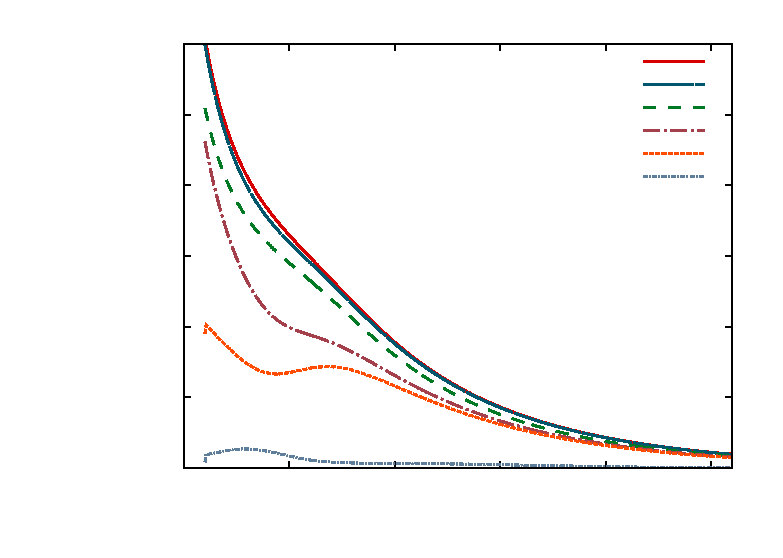
\includegraphics{img/PqdotNormsProjection}}%
    \gplfronttext
  \end{picture}%
\endgroup

    }
\end{center}
\caption{Evolution of the norm of the motion after successively projecting the motion in the
	tasks null spaces.}
\label{fig:xp3Pqdot}
\end{figure}
Each projection strictly decreases the norm of the velocity (\emph{ie} the quantity of  movement). After
five projections, the movement is completely nullified, which confirms that all the active tasks have been
discovered. The algorithm can then stops.

\subsection{Experiment 2 : Distinction between two close motions}
\label{sec:distinc}
An interesting challenge in motion detection
is to make distinction between two motions
involving different tasks but that produce very similar joint trajectories.
Anthropomorphic algorithm would use the context to perform the disambiguation.
The work presented in this paper shows that the fitting criterion
is sufficient to disambiguate similar-looking motion. Three ambiguous pairs of movements
are presented to illustrate this capability.


\subsubsection{Reaching motions}
\label{sec:distinc1}
In this section, two motions are considered: \emph{motion 2.a} and \emph{motion 2.b}.
The first one is a far-reaching motion with the right hand.
The reaching motion of the right hand has an influence on the left arm through the \emph{Com} task:
to regulate its balance, the robot puts its left arm behind.
The second motion is the same reaching task for the right hand, added with a
second reaching task on the left hand. The desired position of the left
hand is artificially set to the final position of the left hand obtained at the first motion.

The final states of the robot for the two motions are shown in the Fig.~\ref{fig:introExample:spotDiff}.
A video showing those two motions on the HRP-2 is available\footnote{{http://homepages.laas.fr/shak/videos/}}.
The two motions look very similar, and it is very difficult to the human eye
to tell which motion involves a left and right hand task without the context.
In the first case, the motion of the left hand is due to the \emph{Com} and \emph{Right Hand} task, 
as it is a side effect to compensate the balance of the right hand.
In the second case, the motion of the left hand is decoupled,
since the left hand has been driven by its own goal.
However, in the proper task spaces, those motions appear clearly different.
Fig.~\ref{fig:XP2RFit} shows an example of the result of the task fitting of the 
\emph{Right Hand} and \emph{Left Hand} task applied to the \emph{motion 2.a}.
\begin{figure*}[t]
\centering
\begin{tabular*}{0.9\textwidth}{@{\extracolsep{\fill}}cc}
%\includegraphics[width=0.9\linewidth]{img/projRHNull.eps}
  \resizebox{.48\textwidth}{!} {
      % GNUPLOT: LaTeX picture with Postscript
\begingroup
  \makeatletter
  \providecommand\color[2][]{%
    \GenericError{(gnuplot) \space\space\space\@spaces}{%
      Package color not loaded in conjunction with
      terminal option `colourtext'%
    }{See the gnuplot documentation for explanation.%
    }{Either use 'blacktext' in gnuplot or load the package
      color.sty in LaTeX.}%
    \renewcommand\color[2][]{}%
  }%
  \providecommand\includegraphics[2][]{%
    \GenericError{(gnuplot) \space\space\space\@spaces}{%
      Package graphicx or graphics not loaded%
    }{See the gnuplot documentation for explanation.%
    }{The gnuplot epslatex terminal needs graphicx.sty or graphics.sty.}%
    \renewcommand\includegraphics[2][]{}%
  }%
  \providecommand\rotatebox[2]{#2}%
  \@ifundefined{ifGPcolor}{%
    \newif\ifGPcolor
    \GPcolortrue
  }{}%
  \@ifundefined{ifGPblacktext}{%
    \newif\ifGPblacktext
    \GPblacktexttrue
  }{}%
  % define a \g@addto@macro without @ in the name:
  \let\gplgaddtomacro\g@addto@macro
  % define empty templates for all commands taking text:
  \gdef\gplbacktext{}%
  \gdef\gplfronttext{}%
  \makeatother
  \ifGPblacktext
    % no textcolor at all
    \def\colorrgb#1{}%
    \def\colorgray#1{}%
  \else
    % gray or color?
    \ifGPcolor
      \def\colorrgb#1{\color[rgb]{#1}}%
      \def\colorgray#1{\color[gray]{#1}}%
      \expandafter\def\csname LTw\endcsname{\color{white}}%
      \expandafter\def\csname LTb\endcsname{\color{black}}%
      \expandafter\def\csname LTa\endcsname{\color{black}}%
      \expandafter\def\csname LT0\endcsname{\color[rgb]{1,0,0}}%
      \expandafter\def\csname LT1\endcsname{\color[rgb]{0,1,0}}%
      \expandafter\def\csname LT2\endcsname{\color[rgb]{0,0,1}}%
      \expandafter\def\csname LT3\endcsname{\color[rgb]{1,0,1}}%
      \expandafter\def\csname LT4\endcsname{\color[rgb]{0,1,1}}%
      \expandafter\def\csname LT5\endcsname{\color[rgb]{1,1,0}}%
      \expandafter\def\csname LT6\endcsname{\color[rgb]{0,0,0}}%
      \expandafter\def\csname LT7\endcsname{\color[rgb]{1,0.3,0}}%
      \expandafter\def\csname LT8\endcsname{\color[rgb]{0.5,0.5,0.5}}%
    \else
      % gray
      \def\colorrgb#1{\color{black}}%
      \def\colorgray#1{\color[gray]{#1}}%
      \expandafter\def\csname LTw\endcsname{\color{white}}%
      \expandafter\def\csname LTb\endcsname{\color{black}}%
      \expandafter\def\csname LTa\endcsname{\color{black}}%
      \expandafter\def\csname LT0\endcsname{\color{black}}%
      \expandafter\def\csname LT1\endcsname{\color{black}}%
      \expandafter\def\csname LT2\endcsname{\color{black}}%
      \expandafter\def\csname LT3\endcsname{\color{black}}%
      \expandafter\def\csname LT4\endcsname{\color{black}}%
      \expandafter\def\csname LT5\endcsname{\color{black}}%
      \expandafter\def\csname LT6\endcsname{\color{black}}%
      \expandafter\def\csname LT7\endcsname{\color{black}}%
      \expandafter\def\csname LT8\endcsname{\color{black}}%
    \fi
  \fi
  \setlength{\unitlength}{0.0500bp}%
  \begin{picture}(7200.00,5040.00)%
    \gplgaddtomacro\gplbacktext{%
      \csname LTb\endcsname%
      \put(990,704){\makebox(0,0)[r]{\strut{} 0}}%
      \put(990,1136){\makebox(0,0)[r]{\strut{} 0.2}}%
      \put(990,1569){\makebox(0,0)[r]{\strut{} 0.4}}%
      \put(990,2001){\makebox(0,0)[r]{\strut{} 0.6}}%
      \put(990,2434){\makebox(0,0)[r]{\strut{} 0.8}}%
      \put(990,2866){\makebox(0,0)[r]{\strut{} 1}}%
      \put(990,3299){\makebox(0,0)[r]{\strut{} 1.2}}%
      \put(990,3731){\makebox(0,0)[r]{\strut{} 1.4}}%
      \put(990,4164){\makebox(0,0)[r]{\strut{} 1.6}}%
      \put(1122,484){\makebox(0,0){\strut{} 0}}%
      \put(1937,484){\makebox(0,0){\strut{} 0.5}}%
      \put(2753,484){\makebox(0,0){\strut{} 1}}%
      \put(3568,484){\makebox(0,0){\strut{} 1.5}}%
      \put(4383,484){\makebox(0,0){\strut{} 2}}%
      \put(5199,484){\makebox(0,0){\strut{} 2.5}}%
      \put(6014,484){\makebox(0,0){\strut{} 3}}%
      \put(6829,484){\makebox(0,0){\strut{} 3.5}}%
      \put(3996,154){\makebox(0,0){\strut{}$t$ (s)}}%
      \put(3996,4710){\makebox(0,0){\strut{}$\begin{array}{rl} r &= 0.147227\\ \int \Vert \mathbf{J}^+ \mathbf{\dot{e}}_{taskRhand} \Vert \mathrm{d}t &=  0.40304 \mathrm{rad}\\ \end{array}$}}%
    }%
    \gplgaddtomacro\gplfronttext{%
      \csname LTb\endcsname%
      \put(5883,4207){\makebox(0,0)[r]{\strut{}$\Vert \mathbf{J}^+ \mathbf{\dot{e}}_{taskRhand} \Vert / \int \Vert \mathbf{J}^+ \mathbf{\dot{e}}_{taskRhand} \Vert \mathrm{d}t$}}%
      \csname LTb\endcsname%
      \put(5883,3987){\makebox(0,0)[r]{\strut{}Model}}%
    }%
    \gplbacktext
    \put(0,0){\includegraphics{img/simu/2a/taskRhandNormInvJerr_0}}%
    \gplfronttext
  \end{picture}%
\endgroup

    }          &
  \resizebox{.48\textwidth}{!} {
      % GNUPLOT: LaTeX picture with Postscript
\begingroup
  \makeatletter
  \providecommand\color[2][]{%
    \GenericError{(gnuplot) \space\space\space\@spaces}{%
      Package color not loaded in conjunction with
      terminal option `colourtext'%
    }{See the gnuplot documentation for explanation.%
    }{Either use 'blacktext' in gnuplot or load the package
      color.sty in LaTeX.}%
    \renewcommand\color[2][]{}%
  }%
  \providecommand\includegraphics[2][]{%
    \GenericError{(gnuplot) \space\space\space\@spaces}{%
      Package graphicx or graphics not loaded%
    }{See the gnuplot documentation for explanation.%
    }{The gnuplot epslatex terminal needs graphicx.sty or graphics.sty.}%
    \renewcommand\includegraphics[2][]{}%
  }%
  \providecommand\rotatebox[2]{#2}%
  \@ifundefined{ifGPcolor}{%
    \newif\ifGPcolor
    \GPcolortrue
  }{}%
  \@ifundefined{ifGPblacktext}{%
    \newif\ifGPblacktext
    \GPblacktexttrue
  }{}%
  % define a \g@addto@macro without @ in the name:
  \let\gplgaddtomacro\g@addto@macro
  % define empty templates for all commands taking text:
  \gdef\gplbacktext{}%
  \gdef\gplfronttext{}%
  \makeatother
  \ifGPblacktext
    % no textcolor at all
    \def\colorrgb#1{}%
    \def\colorgray#1{}%
  \else
    % gray or color?
    \ifGPcolor
      \def\colorrgb#1{\color[rgb]{#1}}%
      \def\colorgray#1{\color[gray]{#1}}%
      \expandafter\def\csname LTw\endcsname{\color{white}}%
      \expandafter\def\csname LTb\endcsname{\color{black}}%
      \expandafter\def\csname LTa\endcsname{\color{black}}%
      \expandafter\def\csname LT0\endcsname{\color[rgb]{1,0,0}}%
      \expandafter\def\csname LT1\endcsname{\color[rgb]{0,1,0}}%
      \expandafter\def\csname LT2\endcsname{\color[rgb]{0,0,1}}%
      \expandafter\def\csname LT3\endcsname{\color[rgb]{1,0,1}}%
      \expandafter\def\csname LT4\endcsname{\color[rgb]{0,1,1}}%
      \expandafter\def\csname LT5\endcsname{\color[rgb]{1,1,0}}%
      \expandafter\def\csname LT6\endcsname{\color[rgb]{0,0,0}}%
      \expandafter\def\csname LT7\endcsname{\color[rgb]{1,0.3,0}}%
      \expandafter\def\csname LT8\endcsname{\color[rgb]{0.5,0.5,0.5}}%
    \else
      % gray
      \def\colorrgb#1{\color{black}}%
      \def\colorgray#1{\color[gray]{#1}}%
      \expandafter\def\csname LTw\endcsname{\color{white}}%
      \expandafter\def\csname LTb\endcsname{\color{black}}%
      \expandafter\def\csname LTa\endcsname{\color{black}}%
      \expandafter\def\csname LT0\endcsname{\color{black}}%
      \expandafter\def\csname LT1\endcsname{\color{black}}%
      \expandafter\def\csname LT2\endcsname{\color{black}}%
      \expandafter\def\csname LT3\endcsname{\color{black}}%
      \expandafter\def\csname LT4\endcsname{\color{black}}%
      \expandafter\def\csname LT5\endcsname{\color{black}}%
      \expandafter\def\csname LT6\endcsname{\color{black}}%
      \expandafter\def\csname LT7\endcsname{\color{black}}%
      \expandafter\def\csname LT8\endcsname{\color{black}}%
    \fi
  \fi
  \setlength{\unitlength}{0.0500bp}%
  \begin{picture}(7200.00,5040.00)%
    \gplgaddtomacro\gplbacktext{%
      \csname LTb\endcsname%
      \put(990,704){\makebox(0,0)[r]{\strut{} 0}}%
      \put(990,1136){\makebox(0,0)[r]{\strut{} 0.2}}%
      \put(990,1569){\makebox(0,0)[r]{\strut{} 0.4}}%
      \put(990,2001){\makebox(0,0)[r]{\strut{} 0.6}}%
      \put(990,2434){\makebox(0,0)[r]{\strut{} 0.8}}%
      \put(990,2866){\makebox(0,0)[r]{\strut{} 1}}%
      \put(990,3299){\makebox(0,0)[r]{\strut{} 1.2}}%
      \put(990,3731){\makebox(0,0)[r]{\strut{} 1.4}}%
      \put(990,4164){\makebox(0,0)[r]{\strut{} 1.6}}%
      \put(1122,484){\makebox(0,0){\strut{} 0}}%
      \put(1937,484){\makebox(0,0){\strut{} 0.5}}%
      \put(2753,484){\makebox(0,0){\strut{} 1}}%
      \put(3568,484){\makebox(0,0){\strut{} 1.5}}%
      \put(4383,484){\makebox(0,0){\strut{} 2}}%
      \put(5199,484){\makebox(0,0){\strut{} 2.5}}%
      \put(6014,484){\makebox(0,0){\strut{} 3}}%
      \put(6829,484){\makebox(0,0){\strut{} 3.5}}%
      \put(3996,154){\makebox(0,0){\strut{}$t$ (s)}}%
      \put(3996,4710){\makebox(0,0){\strut{}$\begin{array}{rl} r &= 2.61576\\ \int \Vert \mathbf{J}^+ \mathbf{\dot{e}}_{taskLhand} \Vert \mathrm{d}t &=  0.189581 \mathrm{rad}\\ \end{array}$}}%
    }%
    \gplgaddtomacro\gplfronttext{%
      \csname LTb\endcsname%
      \put(5883,4207){\makebox(0,0)[r]{\strut{}$\Vert \mathbf{J}^+ \mathbf{\dot{e}}_{taskLhand} \Vert / \int \Vert \mathbf{J}^+ \mathbf{\dot{e}}_{taskLhand} \Vert \mathrm{d}t$}}%
      \csname LTb\endcsname%
      \put(5883,3987){\makebox(0,0)[r]{\strut{}Model}}%
    }%
    \gplbacktext
    \put(0,0){\includegraphics{img/simu/2a/taskLhandNormInvJerr_0}}%
    \gplfronttext
  \end{picture}%
\endgroup

    }\\
\end{tabular*}
\caption{Task fitting on the \emph{motion 2.a} on the right and the left hand tasks. Variable $r$ is the residue,
\emph{ie} the distance between the two curves. The \emph{Right Hand} motion is properly fitted by
the task model, showing that the task is active. The \emph{Left Hand} is not fitted properly, since the task is 
not active. The two cases are easily distinguished by the residue value.} 
\label{fig:XP2RFit}
\end{figure*}
The residue of the optimization is high since the fitting is not possible on a 
trajectory that does not respect the model (in particular, the residue of the \emph{Left Hand} is 
much higher than the \emph{Right Hand}).
Both tasks are properly fitted, and will be detected.
The results of the detection algorithm
are showed in Table~\ref{tab:spotDiff1}.
\begin{table}[h]
\centering
\begin{tabular}{|c|c|c|c|}
\hline
Reference & Detected & $\int \Vert \dot{q}(t) \Vert ^2 dt$ & $\int \Vert P\dot{q}(t) \Vert ^2 dt$ \\
\hline
\begin{tabular}{c}
Com\\
Right Hand\\
Twofeet\\
\end{tabular}

&

\begin{tabular}{c}
Com\\
Right Hand\\
Twofeet\\
\end{tabular}

& 0.364398 & 0.00159355 \\
\hline
\begin{tabular}{c}
Com\\
Left Hand\\
Right Hand\\
Twofeet\\
\end{tabular}

&
\begin{tabular}{c}
Com\\
Left Hand\\
Right Hand\\
Twofeet\\
\end{tabular}

& 0.538329  & 0.0035343 \\
\hline
\end{tabular}
\caption{Results of the task selection algorithm from the analysis of the \emph{motion 2.a} and the \emph{motion 2.b}.}
\label{tab:spotDiff1}
\vspace{-20pt}
\end{table}
The first column shows the
tasks being used in the reference motion, the second column shows the tasks
selected by the algorithm, the third column shows the norm of the reference motion (quantity of motion
initially observed),
and the last column shows the norm of the reference motion projected onto the null space of
all selected tasks. The final quantity of movement
after projection is very low for both motions compared
to the threshold for the stop criterion $\int \Vert P\dot{q}(t) \Vert ^2 dt > \epsilon$
that is fixed to $\epsilon = 0.07$.

Finally Fig.~\ref{fig:RbeforeAfterProj} shows how the norm of joint-angle velocities corresponding to the tasks
\emph{Right Grab} and \emph{Left Grab} evolves after the projections.
\begin{figure*}[t]
\centering
  \subfigure[Motion 2.a]{
  \resizebox{.48\textwidth}{!} {
      % GNUPLOT: LaTeX picture with Postscript
\begingroup
  \makeatletter
  \providecommand\color[2][]{%
    \GenericError{(gnuplot) \space\space\space\@spaces}{%
      Package color not loaded in conjunction with
      terminal option `colourtext'%
    }{See the gnuplot documentation for explanation.%
    }{Either use 'blacktext' in gnuplot or load the package
      color.sty in LaTeX.}%
    \renewcommand\color[2][]{}%
  }%
  \providecommand\includegraphics[2][]{%
    \GenericError{(gnuplot) \space\space\space\@spaces}{%
      Package graphicx or graphics not loaded%
    }{See the gnuplot documentation for explanation.%
    }{The gnuplot epslatex terminal needs graphicx.sty or graphics.sty.}%
    \renewcommand\includegraphics[2][]{}%
  }%
  \providecommand\rotatebox[2]{#2}%
  \@ifundefined{ifGPcolor}{%
    \newif\ifGPcolor
    \GPcolortrue
  }{}%
  \@ifundefined{ifGPblacktext}{%
    \newif\ifGPblacktext
    \GPblacktexttrue
  }{}%
  % define a \g@addto@macro without @ in the name:
  \let\gplgaddtomacro\g@addto@macro
  % define empty templates for all commands taking text:
  \gdef\gplbacktext{}%
  \gdef\gplfronttext{}%
  \makeatother
  \ifGPblacktext
    % no textcolor at all
    \def\colorrgb#1{}%
    \def\colorgray#1{}%
  \else
    % gray or color?
    \ifGPcolor
      \def\colorrgb#1{\color[rgb]{#1}}%
      \def\colorgray#1{\color[gray]{#1}}%
      \expandafter\def\csname LTw\endcsname{\color{white}}%
      \expandafter\def\csname LTb\endcsname{\color{black}}%
      \expandafter\def\csname LTa\endcsname{\color{black}}%
      \expandafter\def\csname LT0\endcsname{\color[rgb]{1,0,0}}%
      \expandafter\def\csname LT1\endcsname{\color[rgb]{0,1,0}}%
      \expandafter\def\csname LT2\endcsname{\color[rgb]{0,0,1}}%
      \expandafter\def\csname LT3\endcsname{\color[rgb]{1,0,1}}%
      \expandafter\def\csname LT4\endcsname{\color[rgb]{0,1,1}}%
      \expandafter\def\csname LT5\endcsname{\color[rgb]{1,1,0}}%
      \expandafter\def\csname LT6\endcsname{\color[rgb]{0,0,0}}%
      \expandafter\def\csname LT7\endcsname{\color[rgb]{1,0.3,0}}%
      \expandafter\def\csname LT8\endcsname{\color[rgb]{0.5,0.5,0.5}}%
    \else
      % gray
      \def\colorrgb#1{\color{black}}%
      \def\colorgray#1{\color[gray]{#1}}%
      \expandafter\def\csname LTw\endcsname{\color{white}}%
      \expandafter\def\csname LTb\endcsname{\color{black}}%
      \expandafter\def\csname LTa\endcsname{\color{black}}%
      \expandafter\def\csname LT0\endcsname{\color{black}}%
      \expandafter\def\csname LT1\endcsname{\color{black}}%
      \expandafter\def\csname LT2\endcsname{\color{black}}%
      \expandafter\def\csname LT3\endcsname{\color{black}}%
      \expandafter\def\csname LT4\endcsname{\color{black}}%
      \expandafter\def\csname LT5\endcsname{\color{black}}%
      \expandafter\def\csname LT6\endcsname{\color{black}}%
      \expandafter\def\csname LT7\endcsname{\color{black}}%
      \expandafter\def\csname LT8\endcsname{\color{black}}%
    \fi
  \fi
  \setlength{\unitlength}{0.0500bp}%
  \begin{picture}(7200.00,5040.00)%
    \gplgaddtomacro\gplbacktext{%
      \csname LTb\endcsname%
      \put(1342,704){\makebox(0,0)[r]{\strut{} 0}}%
      \put(1342,1156){\makebox(0,0)[r]{\strut{} 0.05}}%
      \put(1342,1609){\makebox(0,0)[r]{\strut{} 0.1}}%
      \put(1342,2061){\makebox(0,0)[r]{\strut{} 0.15}}%
      \put(1342,2514){\makebox(0,0)[r]{\strut{} 0.2}}%
      \put(1342,2966){\makebox(0,0)[r]{\strut{} 0.25}}%
      \put(1342,3419){\makebox(0,0)[r]{\strut{} 0.3}}%
      \put(1342,3871){\makebox(0,0)[r]{\strut{} 0.35}}%
      \put(1342,4324){\makebox(0,0)[r]{\strut{} 0.4}}%
      \put(1342,4776){\makebox(0,0)[r]{\strut{} 0.45}}%
      \put(1474,484){\makebox(0,0){\strut{} 0}}%
      \put(2235,484){\makebox(0,0){\strut{} 0.5}}%
      \put(2996,484){\makebox(0,0){\strut{} 1}}%
      \put(3757,484){\makebox(0,0){\strut{} 1.5}}%
      \put(4518,484){\makebox(0,0){\strut{} 2}}%
      \put(5279,484){\makebox(0,0){\strut{} 2.5}}%
      \put(6040,484){\makebox(0,0){\strut{} 3}}%
      \put(6802,484){\makebox(0,0){\strut{} 3.5}}%
      \put(440,2740){\rotatebox{90}{\makebox(0,0){\strut{}$\Vert \mathbf{\dot{q}} \Vert$ (rad/s)}}}%
      \put(4172,154){\makebox(0,0){\strut{}$t$ (s)}}%
    }%
    \gplgaddtomacro\gplfronttext{%
      \csname LTb\endcsname%
      \put(5883,4603){\makebox(0,0)[r]{\strut{}$\Vert \mathbf{J}_{rhand}^+\mathbf{J}_{rhand} \mathbf{\dot{q}} \Vert$}}%
      \csname LTb\endcsname%
      \put(5883,4383){\makebox(0,0)[r]{\strut{}$\Vert \mathbf{J}_{rhand}^+\mathbf{J}_{rhand} \mathbf{P}_{rhand} \mathbf{\dot{q}} \Vert$}}%
      \csname LTb\endcsname%
      \put(5883,4163){\makebox(0,0)[r]{\strut{}$\Vert \mathbf{J}_{rhand}^+\mathbf{J}_{rhand} \mathbf{P}_{rhand+com} \mathbf{\dot{q}} \Vert$}}%
      \csname LTb\endcsname%
      \put(5883,3943){\makebox(0,0)[r]{\strut{}$\Vert \mathbf{J}_{lhand}^+\mathbf{J}_{lhand} \mathbf{\dot{q}} \Vert$}}%
      \csname LTb\endcsname%
      \put(5883,3723){\makebox(0,0)[r]{\strut{}$\Vert \mathbf{J}_{lhand}^+\mathbf{J}_{lhand} \mathbf{P}_{rhand} \mathbf{\dot{q}} \Vert$}}%
      \csname LTb\endcsname%
      \put(5883,3503){\makebox(0,0)[r]{\strut{}$\Vert \mathbf{J}_{lhand}^+\mathbf{J}_{lhand} \mathbf{P}_{rhand+com} \mathbf{\dot{q}} \Vert$}}%
    }%
    \gplbacktext
    \put(0,0){\includegraphics{img/simu/2a/RbeforeAfterProj}}%
    \gplfronttext
  \end{picture}%
\endgroup

    }
  \label{fig:RbeforeAfterProj:2a}
  }
  \subfigure[Motion 2.b]{
  \resizebox{.48\textwidth}{!} {
      % GNUPLOT: LaTeX picture with Postscript
\begingroup
  \makeatletter
  \providecommand\color[2][]{%
    \GenericError{(gnuplot) \space\space\space\@spaces}{%
      Package color not loaded in conjunction with
      terminal option `colourtext'%
    }{See the gnuplot documentation for explanation.%
    }{Either use 'blacktext' in gnuplot or load the package
      color.sty in LaTeX.}%
    \renewcommand\color[2][]{}%
  }%
  \providecommand\includegraphics[2][]{%
    \GenericError{(gnuplot) \space\space\space\@spaces}{%
      Package graphicx or graphics not loaded%
    }{See the gnuplot documentation for explanation.%
    }{The gnuplot epslatex terminal needs graphicx.sty or graphics.sty.}%
    \renewcommand\includegraphics[2][]{}%
  }%
  \providecommand\rotatebox[2]{#2}%
  \@ifundefined{ifGPcolor}{%
    \newif\ifGPcolor
    \GPcolortrue
  }{}%
  \@ifundefined{ifGPblacktext}{%
    \newif\ifGPblacktext
    \GPblacktexttrue
  }{}%
  % define a \g@addto@macro without @ in the name:
  \let\gplgaddtomacro\g@addto@macro
  % define empty templates for all commands taking text:
  \gdef\gplbacktext{}%
  \gdef\gplfronttext{}%
  \makeatother
  \ifGPblacktext
    % no textcolor at all
    \def\colorrgb#1{}%
    \def\colorgray#1{}%
  \else
    % gray or color?
    \ifGPcolor
      \def\colorrgb#1{\color[rgb]{#1}}%
      \def\colorgray#1{\color[gray]{#1}}%
      \expandafter\def\csname LTw\endcsname{\color{white}}%
      \expandafter\def\csname LTb\endcsname{\color{black}}%
      \expandafter\def\csname LTa\endcsname{\color{black}}%
      \expandafter\def\csname LT0\endcsname{\color[rgb]{1,0,0}}%
      \expandafter\def\csname LT1\endcsname{\color[rgb]{0,1,0}}%
      \expandafter\def\csname LT2\endcsname{\color[rgb]{0,0,1}}%
      \expandafter\def\csname LT3\endcsname{\color[rgb]{1,0,1}}%
      \expandafter\def\csname LT4\endcsname{\color[rgb]{0,1,1}}%
      \expandafter\def\csname LT5\endcsname{\color[rgb]{1,1,0}}%
      \expandafter\def\csname LT6\endcsname{\color[rgb]{0,0,0}}%
      \expandafter\def\csname LT7\endcsname{\color[rgb]{1,0.3,0}}%
      \expandafter\def\csname LT8\endcsname{\color[rgb]{0.5,0.5,0.5}}%
    \else
      % gray
      \def\colorrgb#1{\color{black}}%
      \def\colorgray#1{\color[gray]{#1}}%
      \expandafter\def\csname LTw\endcsname{\color{white}}%
      \expandafter\def\csname LTb\endcsname{\color{black}}%
      \expandafter\def\csname LTa\endcsname{\color{black}}%
      \expandafter\def\csname LT0\endcsname{\color{black}}%
      \expandafter\def\csname LT1\endcsname{\color{black}}%
      \expandafter\def\csname LT2\endcsname{\color{black}}%
      \expandafter\def\csname LT3\endcsname{\color{black}}%
      \expandafter\def\csname LT4\endcsname{\color{black}}%
      \expandafter\def\csname LT5\endcsname{\color{black}}%
      \expandafter\def\csname LT6\endcsname{\color{black}}%
      \expandafter\def\csname LT7\endcsname{\color{black}}%
      \expandafter\def\csname LT8\endcsname{\color{black}}%
    \fi
  \fi
  \setlength{\unitlength}{0.0500bp}%
  \begin{picture}(7200.00,5040.00)%
    \gplgaddtomacro\gplbacktext{%
      \csname LTb\endcsname%
      \put(1342,704){\makebox(0,0)[r]{\strut{} 0}}%
      \put(1342,1156){\makebox(0,0)[r]{\strut{} 0.05}}%
      \put(1342,1609){\makebox(0,0)[r]{\strut{} 0.1}}%
      \put(1342,2061){\makebox(0,0)[r]{\strut{} 0.15}}%
      \put(1342,2514){\makebox(0,0)[r]{\strut{} 0.2}}%
      \put(1342,2966){\makebox(0,0)[r]{\strut{} 0.25}}%
      \put(1342,3419){\makebox(0,0)[r]{\strut{} 0.3}}%
      \put(1342,3871){\makebox(0,0)[r]{\strut{} 0.35}}%
      \put(1342,4324){\makebox(0,0)[r]{\strut{} 0.4}}%
      \put(1342,4776){\makebox(0,0)[r]{\strut{} 0.45}}%
      \put(1474,484){\makebox(0,0){\strut{} 0}}%
      \put(2235,484){\makebox(0,0){\strut{} 0.5}}%
      \put(2996,484){\makebox(0,0){\strut{} 1}}%
      \put(3757,484){\makebox(0,0){\strut{} 1.5}}%
      \put(4518,484){\makebox(0,0){\strut{} 2}}%
      \put(5279,484){\makebox(0,0){\strut{} 2.5}}%
      \put(6040,484){\makebox(0,0){\strut{} 3}}%
      \put(6802,484){\makebox(0,0){\strut{} 3.5}}%
      \put(440,2740){\rotatebox{90}{\makebox(0,0){\strut{}$\Vert \mathbf{\dot{q}} \Vert$ (rad/s)}}}%
      \put(4172,154){\makebox(0,0){\strut{}$t$ (s)}}%
    }%
    \gplgaddtomacro\gplfronttext{%
      \csname LTb\endcsname%
      \put(5883,4603){\makebox(0,0)[r]{\strut{}$\Vert \mathbf{J}_{rhand}^+\mathbf{J}_{rhand} \mathbf{\dot{q}} \Vert$}}%
      \csname LTb\endcsname%
      \put(5883,4383){\makebox(0,0)[r]{\strut{}$\Vert \mathbf{J}_{rhand}^+\mathbf{J}_{rhand} \mathbf{P}_{rhand} \mathbf{\dot{q}} \Vert$}}%
      \csname LTb\endcsname%
      \put(5883,4163){\makebox(0,0)[r]{\strut{}$\Vert \mathbf{J}_{rhand}^+\mathbf{J}_{rhand} \mathbf{P}_{rhand+com} \mathbf{\dot{q}} \Vert$}}%
      \csname LTb\endcsname%
      \put(5883,3943){\makebox(0,0)[r]{\strut{}$\Vert \mathbf{J}_{lhand}^+\mathbf{J}_{lhand} \mathbf{\dot{q}} \Vert$}}%
      \csname LTb\endcsname%
      \put(5883,3723){\makebox(0,0)[r]{\strut{}$\Vert \mathbf{J}_{lhand}^+\mathbf{J}_{lhand} \mathbf{P}_{rhand} \mathbf{\dot{q}} \Vert$}}%
      \csname LTb\endcsname%
      \put(5883,3503){\makebox(0,0)[r]{\strut{}$\Vert \mathbf{J}_{lhand}^+\mathbf{J}_{lhand} \mathbf{P}_{rhand+com} \mathbf{\dot{q}} \Vert$}}%
    }%
    \gplbacktext
    \put(0,0){\includegraphics{img/simu/2b/RbeforeAfterProj}}%
    \gplfronttext
  \end{picture}%
\endgroup

  }
  \label{fig:RbeforeAfterProj:2b}
  }
  \caption{Evolution of the trajectory $\dot{\mbf{q}}$ projected in the spaces of
  the \emph{right grab} (in solid lines) and 
  \emph{left grab} (in dashed lines) after
  successive projection of the motion in the nullspace of the task \emph{Right Grab} and in the nullspace
  of the task \emph{Com}. In the \emph{motion 2.a}, a great part of the motion of the left arm is due to 
  the \emph{Com} task: removing the \emph{Com} task will cancel almost all motion in the left arm.
  In the \emph{motion 2.b}, the motion of the left arm is not only involved by the \emph{Com} task
  but mainly by the \emph{Left Grab} task. Removing the \emph{Com} task will only
  cancel a small part of the motion of the left arm.}
\label{fig:RbeforeAfterProj}
\end{figure*}
Projecting the \emph{motion 2.a} onto the null spaces of
the \emph{Right Grab} task will decrease its associated theoretical joint-angle velocities while leaving the
\emph{Left Grab} one unchanged. Fig.~\ref{fig:RbeforeAfterProj:2a} shows
that the theoretical joint-angle velocities associated to the
\emph{Left Grab} task is decreased after the projection of the motion in
the nullspace of the \emph{Com} task.  That explicits that
the left arm of the robot was moved by the \emph{Com} task.
By the way, the projection prevent the left task to be detected at any further iteration of
the algorithm.
But, when projecting the \emph{motion 2.b} into the nullspace of the \emph{Right Grab}
and \emph{Com} task the joint-angle velocities associated to the \emph{Left Grab} task
is still significant (Fig.~\ref{fig:RbeforeAfterProj:2b}). That means that the
\emph{Com} task has a little influence on the
motion of the left arm, and that motion on the left arm is due
to another task. Therefore, the task selection algorithm will keep looking
for the task that has controlled the left arm.
After the detection of the two (for the \emph{motion 2.a}) and three (for \emph{motion 2.b}) main tasks,
the norm of the last joint-angle velocities are not null, because 
the task selection algorithm has not finished and other tasks have not been selected yet.
The \emph{Twofeet} task is then detected but the projection is not displayed on the figure for the sake of clarity.
On the other hand Fig.~\ref{fig:XP2RLFit} shows the task fitting for the \emph{motion 2.b}.

\begin{figure*}[t]
\centering
\begin{tabular*}{0.9\textwidth}{@{\extracolsep{\fill}}cc}
%\includegraphics[width=0.9\linewidth]{img/projRHNull.eps}
  \resizebox{.48\textwidth}{!} {
      % GNUPLOT: LaTeX picture with Postscript
\begingroup
  \makeatletter
  \providecommand\color[2][]{%
    \GenericError{(gnuplot) \space\space\space\@spaces}{%
      Package color not loaded in conjunction with
      terminal option `colourtext'%
    }{See the gnuplot documentation for explanation.%
    }{Either use 'blacktext' in gnuplot or load the package
      color.sty in LaTeX.}%
    \renewcommand\color[2][]{}%
  }%
  \providecommand\includegraphics[2][]{%
    \GenericError{(gnuplot) \space\space\space\@spaces}{%
      Package graphicx or graphics not loaded%
    }{See the gnuplot documentation for explanation.%
    }{The gnuplot epslatex terminal needs graphicx.sty or graphics.sty.}%
    \renewcommand\includegraphics[2][]{}%
  }%
  \providecommand\rotatebox[2]{#2}%
  \@ifundefined{ifGPcolor}{%
    \newif\ifGPcolor
    \GPcolortrue
  }{}%
  \@ifundefined{ifGPblacktext}{%
    \newif\ifGPblacktext
    \GPblacktexttrue
  }{}%
  % define a \g@addto@macro without @ in the name:
  \let\gplgaddtomacro\g@addto@macro
  % define empty templates for all commands taking text:
  \gdef\gplbacktext{}%
  \gdef\gplfronttext{}%
  \makeatother
  \ifGPblacktext
    % no textcolor at all
    \def\colorrgb#1{}%
    \def\colorgray#1{}%
  \else
    % gray or color?
    \ifGPcolor
      \def\colorrgb#1{\color[rgb]{#1}}%
      \def\colorgray#1{\color[gray]{#1}}%
      \expandafter\def\csname LTw\endcsname{\color{white}}%
      \expandafter\def\csname LTb\endcsname{\color{black}}%
      \expandafter\def\csname LTa\endcsname{\color{black}}%
      \expandafter\def\csname LT0\endcsname{\color[rgb]{1,0,0}}%
      \expandafter\def\csname LT1\endcsname{\color[rgb]{0,1,0}}%
      \expandafter\def\csname LT2\endcsname{\color[rgb]{0,0,1}}%
      \expandafter\def\csname LT3\endcsname{\color[rgb]{1,0,1}}%
      \expandafter\def\csname LT4\endcsname{\color[rgb]{0,1,1}}%
      \expandafter\def\csname LT5\endcsname{\color[rgb]{1,1,0}}%
      \expandafter\def\csname LT6\endcsname{\color[rgb]{0,0,0}}%
      \expandafter\def\csname LT7\endcsname{\color[rgb]{1,0.3,0}}%
      \expandafter\def\csname LT8\endcsname{\color[rgb]{0.5,0.5,0.5}}%
    \else
      % gray
      \def\colorrgb#1{\color{black}}%
      \def\colorgray#1{\color[gray]{#1}}%
      \expandafter\def\csname LTw\endcsname{\color{white}}%
      \expandafter\def\csname LTb\endcsname{\color{black}}%
      \expandafter\def\csname LTa\endcsname{\color{black}}%
      \expandafter\def\csname LT0\endcsname{\color{black}}%
      \expandafter\def\csname LT1\endcsname{\color{black}}%
      \expandafter\def\csname LT2\endcsname{\color{black}}%
      \expandafter\def\csname LT3\endcsname{\color{black}}%
      \expandafter\def\csname LT4\endcsname{\color{black}}%
      \expandafter\def\csname LT5\endcsname{\color{black}}%
      \expandafter\def\csname LT6\endcsname{\color{black}}%
      \expandafter\def\csname LT7\endcsname{\color{black}}%
      \expandafter\def\csname LT8\endcsname{\color{black}}%
    \fi
  \fi
  \setlength{\unitlength}{0.0500bp}%
  \begin{picture}(7200.00,5040.00)%
    \gplgaddtomacro\gplbacktext{%
      \csname LTb\endcsname%
      \put(990,704){\makebox(0,0)[r]{\strut{} 0}}%
      \put(990,1136){\makebox(0,0)[r]{\strut{} 0.2}}%
      \put(990,1569){\makebox(0,0)[r]{\strut{} 0.4}}%
      \put(990,2001){\makebox(0,0)[r]{\strut{} 0.6}}%
      \put(990,2434){\makebox(0,0)[r]{\strut{} 0.8}}%
      \put(990,2866){\makebox(0,0)[r]{\strut{} 1}}%
      \put(990,3299){\makebox(0,0)[r]{\strut{} 1.2}}%
      \put(990,3731){\makebox(0,0)[r]{\strut{} 1.4}}%
      \put(990,4164){\makebox(0,0)[r]{\strut{} 1.6}}%
      \put(1122,484){\makebox(0,0){\strut{} 0}}%
      \put(1937,484){\makebox(0,0){\strut{} 0.5}}%
      \put(2753,484){\makebox(0,0){\strut{} 1}}%
      \put(3568,484){\makebox(0,0){\strut{} 1.5}}%
      \put(4383,484){\makebox(0,0){\strut{} 2}}%
      \put(5199,484){\makebox(0,0){\strut{} 2.5}}%
      \put(6014,484){\makebox(0,0){\strut{} 3}}%
      \put(6829,484){\makebox(0,0){\strut{} 3.5}}%
      \put(3996,154){\makebox(0,0){\strut{}$t$ (s)}}%
      \put(3996,4710){\makebox(0,0){\strut{}$\begin{array}{rl} r &= 0.186639\\ \int \Vert \mathbf{J}^+ \mathbf{\dot{e}}_{taskRhand} \Vert \mathrm{d}t &=  0.403712 \mathrm{rad}\\ \end{array}$}}%
    }%
    \gplgaddtomacro\gplfronttext{%
      \csname LTb\endcsname%
      \put(5883,4207){\makebox(0,0)[r]{\strut{}$\Vert \mathbf{J}^+ \mathbf{\dot{e}}_{taskRhand} \Vert / \int \Vert \mathbf{J}^+ \mathbf{\dot{e}}_{taskRhand} \Vert \mathrm{d}t$}}%
      \csname LTb\endcsname%
      \put(5883,3987){\makebox(0,0)[r]{\strut{}Model}}%
    }%
    \gplbacktext
    \put(0,0){\includegraphics{img/simu/2b/taskRhandNormInvJerr_0}}%
    \gplfronttext
  \end{picture}%
\endgroup

    }                           &
  \resizebox{.48\textwidth}{!} {
      % GNUPLOT: LaTeX picture with Postscript
\begingroup
  \makeatletter
  \providecommand\color[2][]{%
    \GenericError{(gnuplot) \space\space\space\@spaces}{%
      Package color not loaded in conjunction with
      terminal option `colourtext'%
    }{See the gnuplot documentation for explanation.%
    }{Either use 'blacktext' in gnuplot or load the package
      color.sty in LaTeX.}%
    \renewcommand\color[2][]{}%
  }%
  \providecommand\includegraphics[2][]{%
    \GenericError{(gnuplot) \space\space\space\@spaces}{%
      Package graphicx or graphics not loaded%
    }{See the gnuplot documentation for explanation.%
    }{The gnuplot epslatex terminal needs graphicx.sty or graphics.sty.}%
    \renewcommand\includegraphics[2][]{}%
  }%
  \providecommand\rotatebox[2]{#2}%
  \@ifundefined{ifGPcolor}{%
    \newif\ifGPcolor
    \GPcolortrue
  }{}%
  \@ifundefined{ifGPblacktext}{%
    \newif\ifGPblacktext
    \GPblacktexttrue
  }{}%
  % define a \g@addto@macro without @ in the name:
  \let\gplgaddtomacro\g@addto@macro
  % define empty templates for all commands taking text:
  \gdef\gplbacktext{}%
  \gdef\gplfronttext{}%
  \makeatother
  \ifGPblacktext
    % no textcolor at all
    \def\colorrgb#1{}%
    \def\colorgray#1{}%
  \else
    % gray or color?
    \ifGPcolor
      \def\colorrgb#1{\color[rgb]{#1}}%
      \def\colorgray#1{\color[gray]{#1}}%
      \expandafter\def\csname LTw\endcsname{\color{white}}%
      \expandafter\def\csname LTb\endcsname{\color{black}}%
      \expandafter\def\csname LTa\endcsname{\color{black}}%
      \expandafter\def\csname LT0\endcsname{\color[rgb]{1,0,0}}%
      \expandafter\def\csname LT1\endcsname{\color[rgb]{0,1,0}}%
      \expandafter\def\csname LT2\endcsname{\color[rgb]{0,0,1}}%
      \expandafter\def\csname LT3\endcsname{\color[rgb]{1,0,1}}%
      \expandafter\def\csname LT4\endcsname{\color[rgb]{0,1,1}}%
      \expandafter\def\csname LT5\endcsname{\color[rgb]{1,1,0}}%
      \expandafter\def\csname LT6\endcsname{\color[rgb]{0,0,0}}%
      \expandafter\def\csname LT7\endcsname{\color[rgb]{1,0.3,0}}%
      \expandafter\def\csname LT8\endcsname{\color[rgb]{0.5,0.5,0.5}}%
    \else
      % gray
      \def\colorrgb#1{\color{black}}%
      \def\colorgray#1{\color[gray]{#1}}%
      \expandafter\def\csname LTw\endcsname{\color{white}}%
      \expandafter\def\csname LTb\endcsname{\color{black}}%
      \expandafter\def\csname LTa\endcsname{\color{black}}%
      \expandafter\def\csname LT0\endcsname{\color{black}}%
      \expandafter\def\csname LT1\endcsname{\color{black}}%
      \expandafter\def\csname LT2\endcsname{\color{black}}%
      \expandafter\def\csname LT3\endcsname{\color{black}}%
      \expandafter\def\csname LT4\endcsname{\color{black}}%
      \expandafter\def\csname LT5\endcsname{\color{black}}%
      \expandafter\def\csname LT6\endcsname{\color{black}}%
      \expandafter\def\csname LT7\endcsname{\color{black}}%
      \expandafter\def\csname LT8\endcsname{\color{black}}%
    \fi
  \fi
  \setlength{\unitlength}{0.0500bp}%
  \begin{picture}(7200.00,5040.00)%
    \gplgaddtomacro\gplbacktext{%
      \csname LTb\endcsname%
      \put(990,704){\makebox(0,0)[r]{\strut{} 0}}%
      \put(990,1136){\makebox(0,0)[r]{\strut{} 0.2}}%
      \put(990,1569){\makebox(0,0)[r]{\strut{} 0.4}}%
      \put(990,2001){\makebox(0,0)[r]{\strut{} 0.6}}%
      \put(990,2434){\makebox(0,0)[r]{\strut{} 0.8}}%
      \put(990,2866){\makebox(0,0)[r]{\strut{} 1}}%
      \put(990,3299){\makebox(0,0)[r]{\strut{} 1.2}}%
      \put(990,3731){\makebox(0,0)[r]{\strut{} 1.4}}%
      \put(990,4164){\makebox(0,0)[r]{\strut{} 1.6}}%
      \put(1122,484){\makebox(0,0){\strut{} 0}}%
      \put(1937,484){\makebox(0,0){\strut{} 0.5}}%
      \put(2753,484){\makebox(0,0){\strut{} 1}}%
      \put(3568,484){\makebox(0,0){\strut{} 1.5}}%
      \put(4383,484){\makebox(0,0){\strut{} 2}}%
      \put(5199,484){\makebox(0,0){\strut{} 2.5}}%
      \put(6014,484){\makebox(0,0){\strut{} 3}}%
      \put(6829,484){\makebox(0,0){\strut{} 3.5}}%
      \put(3996,154){\makebox(0,0){\strut{}$t$ (s)}}%
      \put(3996,4710){\makebox(0,0){\strut{}$\begin{array}{rl} r &= 0.301578\\ \int \Vert \mathbf{J}^+ \mathbf{\dot{e}}_{taskLhand} \Vert \mathrm{d}t &=  0.187033 \mathrm{rad}\\ \end{array}$}}%
    }%
    \gplgaddtomacro\gplfronttext{%
      \csname LTb\endcsname%
      \put(5883,4207){\makebox(0,0)[r]{\strut{}$\Vert \mathbf{J}^+ \mathbf{\dot{e}}_{taskLhand} \Vert / \int \Vert \mathbf{J}^+ \mathbf{\dot{e}}_{taskLhand} \Vert \mathrm{d}t$}}%
      \csname LTb\endcsname%
      \put(5883,3987){\makebox(0,0)[r]{\strut{}Model}}%
    }%
    \gplbacktext
    \put(0,0){\includegraphics{img/simu/2b/taskLhandNormInvJerr_0}}%
    \gplfronttext
  \end{picture}%
\endgroup

    }\\
\end{tabular*}
\caption{Task fitting on the \emph{motion 2.b} on the right and the left hand tasks. Both motion of the right
and left hand are fitted by the model, with small residue: the tasks are detected.}
\label{fig:XP2RLFit}
\end{figure*}

\subsubsection{Grabbing VS Screwing}
\label{sec:distinc2}
In this section, the two motions considered are the \emph{motion 3.a} and \emph{motion 3.b}.
Both motions share the same position target for the right hand. The only difference between
the two demonstrated motions is the
presence of an orientation constraint for the right hand in the \emph{motion 3.b}.
The final positions of those motions are shown in the Fig.~\ref{fig:spotDiff2}.
Table~\ref{tab:spotDiff2} shows the results of the task-selection algorithm which performed successfully.
\begin{table}[h]
  \centering
  \begin{tabular}{|c|c|c|c|}
    \hline
    Reference & Detected & $\int \Vert \dot{q}(t) \Vert ^2 dt$ & $\int \Vert P\dot{q}(t) \Vert ^2 dt$ \\
    \hline
    \begin{tabular}{c}
      Com\\
      Gaze\\
      Grab\\
      Twofeet\\
    \end{tabular}
    &
    \begin{tabular}{c}
      Com\\
      Gaze\\
      Grab\\
      Twofeet\\
    \end{tabular}
    & 0.838686 & 0.0132712 \\
    \hline
    \begin{tabular}{c}
      Com\\
      Gaze\\
      Screw\\
      Twofeet\\
    \end{tabular}
    &
    \begin{tabular}{c}
      Com\\
      Gaze\\
      Screw\\
      Twofeet\\
    \end{tabular}
    & 1.23008 & 0.0170635\\
    \hline
  \end{tabular}
  \caption{Results of the task selection algorithm from the analysis of the
  \emph{motion 3.a} and the \emph{motion 3.b}.}
  \label{tab:spotDiff2}
  \vspace{-3pt}
\end{table}
As in the previous experiments, the task \emph{Screw} can not be properly fitted on the trajectory
generated by the \emph{Grab} task alone. The \emph{Grab} task is then first selected in \emph{motion 3.a}.
The projection nullified the residual motion that could have led to a further wrong detection.
For \emph{motion 3.b}, both tasks \emph{Grab} and \emph{Screw} can be detected.
The residual motion after successive projections is finally very close to 0, which proved that
all tasks were properly detected.
%During the analysis of the \emph{motion 3.b}, the \emph{grabbing} task
%is selected as well since the grab task is
%actually a sub-task of the \emph{screwing} motion. Of course, the \emph{screwing} task is not selected
%in the analysis of the \emph{motion 3.a}.

\subsubsection{Screw VS Gaze}
\label{sec:distinc3}
The two motions considered are the \emph{motion 4.a} and \emph{motion 4.b}.
The \emph{motion 4.a} can be described by the following scenario :
an object is in front of the robot, and creates an occlusion in the vision of the robot.
To get rid of this occlusion, the robot can lean on its right. 
While the robot leans, the left hand is dragged by the chest as an involuntary side effect.
The position and orientation of that hand is recorded as a desired state of the
hand for the first \emph{motion 4.b} task.
In \emph{motion 4.b}, the gaze is uncontrolled. The motion of the head is,
that time, a side effect of the left hand movement.
The final states of the robot are shown in Fig.~\ref{fig:spotDiff3}
and the analysis results are summarized in Table~\ref{tab:spotDiff3}.
\begin{table}[h]
\centering
\begin{tabular}{|c|c|c|c|}
\hline
Reference & Detected & $\int \Vert \dot{q}(t) \Vert ^2 dt$ & $\int \Vert P\dot{q}(t) \Vert ^2 dt$ \\
\hline
\begin{tabular}{c}
Com\\
Gaze\\
Twofeet\\
\end{tabular}

&

\begin{tabular}{c}
Com\\
Gaze\\
Twofeet\\
\end{tabular}

& 0.534478 & 0.0545944 \\
\hline
\begin{tabular}{c}
Com\\
Screw\\
Twofeet\\
\end{tabular}

&
\begin{tabular}{c}
Com\\
Screw\\
Twofeet\\
\end{tabular}

& 0.558084 & 0.0023297\\
\hline
\end{tabular}
\caption{Results of the task selection algorithm from the analysis of the \emph{motion 4.a} and the \emph{motion 4.b}.}
\label{tab:spotDiff3}
\vspace{-12pt}
\end{table}

As previously, correct tasks are detected for each movement. The residue after projections on all detected
tasks are very small, proving that everything was properly detected and subtracted.

In conclusion, we have shown experimentally in this section that, without noise, the detection algorithm
performs perfectly, \emph{ie} detects exactly all the active tasks, without any  false detection,
and issues a neglectable residue of projected motion. The following section will consider
realistic cases of noisy signals acquired by real sensors.

\section{Experimentation on the robot}
\label{sec:real}
\IEEEPARstart{I}{n} this section, we will experimentally demonstrate the validity of the task-recognition algorithm
in realistic situation in presence of noise. This time, the reference motion 
is demonstrated by the real HRP-2 and observed 
using a motion-capture system. (Fig.~\ref{fig:hrp2Markers}).
As previously, the task recognition algorithm is applied to two pairs of similar looking motions.
First time, we will briefly explain how the motion-capture system is used to record the joint-angle 
trajectory. Then two pairs of motions are observed and provided to the recognition algorithm.

\subsection{Experimental setup}\label{sec:xpset}
A motion is executed with the \emph{SoT} on the HRP-2 robot equipped with markers on each
body (see Fig.~\ref{fig:hrp2Markers}).
\begin{figure}[t]
  \centering
  \begin{tabular}{cc}
    \includegraphics[height=0.7\linewidth]{img/hrp2Markers.ps} &
    \includegraphics[height=0.7\linewidth]{img/skel.ps} \\
  \end{tabular}
  \caption{Markers set and virtual skeleton of HRP2.}
  \label{fig:hrp2Markers}
\end{figure}
The motion-capture system used is composed of 10 digital cameras and record data
at 200Hz. 
The motion-capture system provides the trajectory of each body of the robot.
The data collected from those markers
are used to build a virtual skeleton that match the kinematic hierarchy of the robot (Fig.~\ref{fig:hrp2Markers}).
The result of this process is the 6D trajectories of all the bodies in space, without any joint constraints.

The analysis of the motion is performed on the joint-angle trajectories.
Therefore, a joint-angle trajectories have to be computed from the motion-capture data.
The joint-angle trajectories are computed as classically done by optimizing the distance
between the transformation matrix $\tensor[^{W}]{\mathbf{R}}{_{q_i}}(\mbf{q})$ from the 
robot origin to each joint of the robot and the measured
transformation matrix $\tensor[^{W}]{\mathbf{\hat{R}}}{_{q_i}}(t)$ using the robot's joint limits
as constraints. 
\begin{eqnarray}
  \mbf{\hat{q}}(t) =  & \underset{\mbf{q}}\argmin & \sum_i^n \Vert \tensor[^{W}]{\mathbf{\hat{R}}}{_{q_i}}(t) \ominus \tensor[^{W}]{\mathbf{R}}{_{q_i}}(\mbf{q}) \Vert ^2\\
    & \text{s.t.} & q_{i\mathrm{min}} \leq q_i \leq q_{i\mathrm{max}}, \; i = 1..n
  \label{mocapOpti}
\end{eqnarray}
where $\mbf{q}$ is the robot joint configuration vector,
$\ominus$ is the distance operator in SO(3), 
$\tensor[^{W}]{\mathbf{R}}{_{q_i}}(\mbf{q})$ is computed using the kinematic
model of the robot, and $\tensor[^{W}]{\mathbf{\hat{R}}}{_{q_i}}$ is obtained by:
\begin{equation}
  \tensor[^{W}]{\mathbf{\hat{R}}}{_{q_i}}(t) = \tensor[^{W}]{\mathbf{R}}{_{W_{C}}} \times \tensor[^{W_{C}}]{\mathbf{\hat{R}}}{_{M_i}}(t) \times \tensor[^{M_i}]{\mathbf{R}}{_{q_i}}    
  \label{mocapMatrix}
\end{equation}
where $\tensor[^{W}]{\mathbf{R}}{_{W_{C}}}$ and $\tensor[^{M_i}]{\mathbf{R}}{_{q_i}}$ are the constants
displacement due to the differences between an arbitrary skeleton model of the motion-capture and our kinematic model of the robot,
computed in a calibration step.
$\tensor[^{W_{C}}]{\mathbf{\hat{R}}}{_{M_i}}$
is the measured transformation matrix from the origin of the motion-capture reference frame
to the virtual body $i$. 

The obtained joint-angle trajectories are then used for the reverse-engineering task-recognition.\\

On the real robot, a flexibility is introduced after the ankle joint that
interferes with the motion at the very beginning as the acceleration
of the joint-angle increases quickly. The flexibility is not modeled 
neither in the control algorithm nor the detection method.
In order to bypass the influence of the flexibility, the motion analysis is done after the first 100ms
where the influence of the flexibility is predominant.
In the following two sections, we consider that the measures are directly the $\mbf{\hat{q}}$ trajectories
given by equation~(\ref{mocapMatrix}).

\subsection{Grabbing VS Maintaining balance}
This experiment corresponds to the one realized in simulation in section~\ref{sec:distinc1}:
the first motion is a motion of the left arm induced by the coupling between a far reaching of the right hand,
hand the balancing \emph{Com} task (\emph{motion 2.a}). The second motion is a reaching of both hands, built to be 
ambiguous with regard to the first motion~(\emph{motion 2.b} in Table~\ref{tab:motion}).
Table~\ref{tab:spotDiffReal1} shows the result of the identification algorithm for
the \emph{motion 2.a} and the \emph{motion 2.b} with a termination threshold set to $ \epsilon = 0.07$.
\begin{table}[h]
  \centering
  \begin{tabular}{|c|c|c|c|}
    \hline
    Reference & Detected & $\int \Vert \dot{q}(t) \Vert ^2 dt$ & $\int \Vert P\dot{q}(t) \Vert ^2 dt$ \\
    \hline
    \begin{tabular}{c}
      Com\\
      Right grab\\
      Twofeet\\
    \end{tabular}

    &

    \begin{tabular}{c}
      Com\\
      Right grab\\
      Twofeet\\
    \end{tabular}

    & 0.104835 & 0.0482885 \\
    \hline
    \begin{tabular}{c}
      Com\\
      Left grab\\
      Right grab\\
      Twofeet\\
    \end{tabular}

    &
    \begin{tabular}{c}
      Com\\
      Left grab\\
      Right grab\\
      Twofeet\\
    \end{tabular}

    & 0.142293  & 0.0541836 \\
    \hline
  \end{tabular}
  \caption{Results of the task selection algorithm from the analysis of the \emph{motion 2.a} and the \emph{motion 2.b} on the real robot.}
  \label{tab:spotDiffReal1}
  \vspace{-20pt}
\end{table}

For the \emph{motion 2.a}, the order of the task extraction is :
\emph{Right Grab}, \emph{Twofeet} and \emph{Com} task.
Whereas for the \emph{motion 2.b},
the extracted tasks are : \emph{Right Grab},  \emph{Com}, \emph{Twofeet} and \emph{Left Grab}.

Fig.~\ref{fig:exp1:headFit}-\ref{fig:exp1:taskLhand} show the
fitting at the first iteration of the algorithm for the \emph{Head} and \emph{Left Grab} tasks. As expected,
the fitting performs well only for the \emph{Left Grab} task in the \emph{motion 2.b} while it is rejected for
\emph{motion 2.a}.
\begin{figure*}[t]
  \centering
  \subfigure[Motion 2.a]{
  \resizebox{.48\textwidth}{!} {
  % GNUPLOT: LaTeX picture with Postscript
\begingroup
  \makeatletter
  \providecommand\color[2][]{%
    \GenericError{(gnuplot) \space\space\space\@spaces}{%
      Package color not loaded in conjunction with
      terminal option `colourtext'%
    }{See the gnuplot documentation for explanation.%
    }{Either use 'blacktext' in gnuplot or load the package
      color.sty in LaTeX.}%
    \renewcommand\color[2][]{}%
  }%
  \providecommand\includegraphics[2][]{%
    \GenericError{(gnuplot) \space\space\space\@spaces}{%
      Package graphicx or graphics not loaded%
    }{See the gnuplot documentation for explanation.%
    }{The gnuplot epslatex terminal needs graphicx.sty or graphics.sty.}%
    \renewcommand\includegraphics[2][]{}%
  }%
  \providecommand\rotatebox[2]{#2}%
  \@ifundefined{ifGPcolor}{%
    \newif\ifGPcolor
    \GPcolortrue
  }{}%
  \@ifundefined{ifGPblacktext}{%
    \newif\ifGPblacktext
    \GPblacktexttrue
  }{}%
  % define a \g@addto@macro without @ in the name:
  \let\gplgaddtomacro\g@addto@macro
  % define empty templates for all commands taking text:
  \gdef\gplbacktext{}%
  \gdef\gplfronttext{}%
  \makeatother
  \ifGPblacktext
    % no textcolor at all
    \def\colorrgb#1{}%
    \def\colorgray#1{}%
  \else
    % gray or color?
    \ifGPcolor
      \def\colorrgb#1{\color[rgb]{#1}}%
      \def\colorgray#1{\color[gray]{#1}}%
      \expandafter\def\csname LTw\endcsname{\color{white}}%
      \expandafter\def\csname LTb\endcsname{\color{black}}%
      \expandafter\def\csname LTa\endcsname{\color{black}}%
      \expandafter\def\csname LT0\endcsname{\color[rgb]{1,0,0}}%
      \expandafter\def\csname LT1\endcsname{\color[rgb]{0,1,0}}%
      \expandafter\def\csname LT2\endcsname{\color[rgb]{0,0,1}}%
      \expandafter\def\csname LT3\endcsname{\color[rgb]{1,0,1}}%
      \expandafter\def\csname LT4\endcsname{\color[rgb]{0,1,1}}%
      \expandafter\def\csname LT5\endcsname{\color[rgb]{1,1,0}}%
      \expandafter\def\csname LT6\endcsname{\color[rgb]{0,0,0}}%
      \expandafter\def\csname LT7\endcsname{\color[rgb]{1,0.3,0}}%
      \expandafter\def\csname LT8\endcsname{\color[rgb]{0.5,0.5,0.5}}%
    \else
      % gray
      \def\colorrgb#1{\color{black}}%
      \def\colorgray#1{\color[gray]{#1}}%
      \expandafter\def\csname LTw\endcsname{\color{white}}%
      \expandafter\def\csname LTb\endcsname{\color{black}}%
      \expandafter\def\csname LTa\endcsname{\color{black}}%
      \expandafter\def\csname LT0\endcsname{\color{black}}%
      \expandafter\def\csname LT1\endcsname{\color{black}}%
      \expandafter\def\csname LT2\endcsname{\color{black}}%
      \expandafter\def\csname LT3\endcsname{\color{black}}%
      \expandafter\def\csname LT4\endcsname{\color{black}}%
      \expandafter\def\csname LT5\endcsname{\color{black}}%
      \expandafter\def\csname LT6\endcsname{\color{black}}%
      \expandafter\def\csname LT7\endcsname{\color{black}}%
      \expandafter\def\csname LT8\endcsname{\color{black}}%
    \fi
  \fi
  \setlength{\unitlength}{0.0500bp}%
  \begin{picture}(7200.00,5040.00)%
    \gplgaddtomacro\gplbacktext{%
      \csname LTb\endcsname%
      \put(990,704){\makebox(0,0)[r]{\strut{} 0}}%
      \put(990,1439){\makebox(0,0)[r]{\strut{} 0.1}}%
      \put(990,2174){\makebox(0,0)[r]{\strut{} 0.2}}%
      \put(990,2910){\makebox(0,0)[r]{\strut{} 0.3}}%
      \put(990,3645){\makebox(0,0)[r]{\strut{} 0.4}}%
      \put(990,4380){\makebox(0,0)[r]{\strut{} 0.5}}%
      \put(1122,484){\makebox(0,0){\strut{} 0}}%
      \put(2031,484){\makebox(0,0){\strut{} 2}}%
      \put(2940,484){\makebox(0,0){\strut{} 4}}%
      \put(3848,484){\makebox(0,0){\strut{} 6}}%
      \put(4757,484){\makebox(0,0){\strut{} 8}}%
      \put(5666,484){\makebox(0,0){\strut{} 10}}%
      \put(6575,484){\makebox(0,0){\strut{} 12}}%
      \put(3996,154){\makebox(0,0){\strut{}$t$ (s)}}%
      \put(3996,4710){\makebox(0,0){\strut{}$\begin{array}{rl} r &= 2.81934\\ \int \Vert \mathbf{J}^+ \mathbf{\dot{e}}_{taskHead} \Vert \mathrm{d}t &=  0.0355857 \mathrm{rad}\\ \end{array}$}}%
    }%
    \gplgaddtomacro\gplfronttext{%
      \csname LTb\endcsname%
      \put(5883,4207){\makebox(0,0)[r]{\strut{}$\Vert \mathbf{J}^+ \mathbf{\dot{e}}_{taskHead} \Vert / \int \Vert \mathbf{J}^+ \mathbf{\dot{e}}_{taskHead} \Vert \mathrm{d}t$}}%
      \csname LTb\endcsname%
      \put(5883,3987){\makebox(0,0)[r]{\strut{}Model}}%
    }%
    \gplbacktext
    \put(0,0){\includegraphics{img/realRobot/2a/taskHeadNormInvJerr_0}}%
    \gplfronttext
  \end{picture}%
\endgroup

  }
  \label{fig:exp1:headFit:R}
  }
  \subfigure[Motion 2.b]{
  \resizebox{.48\textwidth}{!} {
  % GNUPLOT: LaTeX picture with Postscript
\begingroup
  \makeatletter
  \providecommand\color[2][]{%
    \GenericError{(gnuplot) \space\space\space\@spaces}{%
      Package color not loaded in conjunction with
      terminal option `colourtext'%
    }{See the gnuplot documentation for explanation.%
    }{Either use 'blacktext' in gnuplot or load the package
      color.sty in LaTeX.}%
    \renewcommand\color[2][]{}%
  }%
  \providecommand\includegraphics[2][]{%
    \GenericError{(gnuplot) \space\space\space\@spaces}{%
      Package graphicx or graphics not loaded%
    }{See the gnuplot documentation for explanation.%
    }{The gnuplot epslatex terminal needs graphicx.sty or graphics.sty.}%
    \renewcommand\includegraphics[2][]{}%
  }%
  \providecommand\rotatebox[2]{#2}%
  \@ifundefined{ifGPcolor}{%
    \newif\ifGPcolor
    \GPcolortrue
  }{}%
  \@ifundefined{ifGPblacktext}{%
    \newif\ifGPblacktext
    \GPblacktexttrue
  }{}%
  % define a \g@addto@macro without @ in the name:
  \let\gplgaddtomacro\g@addto@macro
  % define empty templates for all commands taking text:
  \gdef\gplbacktext{}%
  \gdef\gplfronttext{}%
  \makeatother
  \ifGPblacktext
    % no textcolor at all
    \def\colorrgb#1{}%
    \def\colorgray#1{}%
  \else
    % gray or color?
    \ifGPcolor
      \def\colorrgb#1{\color[rgb]{#1}}%
      \def\colorgray#1{\color[gray]{#1}}%
      \expandafter\def\csname LTw\endcsname{\color{white}}%
      \expandafter\def\csname LTb\endcsname{\color{black}}%
      \expandafter\def\csname LTa\endcsname{\color{black}}%
      \expandafter\def\csname LT0\endcsname{\color[rgb]{1,0,0}}%
      \expandafter\def\csname LT1\endcsname{\color[rgb]{0,1,0}}%
      \expandafter\def\csname LT2\endcsname{\color[rgb]{0,0,1}}%
      \expandafter\def\csname LT3\endcsname{\color[rgb]{1,0,1}}%
      \expandafter\def\csname LT4\endcsname{\color[rgb]{0,1,1}}%
      \expandafter\def\csname LT5\endcsname{\color[rgb]{1,1,0}}%
      \expandafter\def\csname LT6\endcsname{\color[rgb]{0,0,0}}%
      \expandafter\def\csname LT7\endcsname{\color[rgb]{1,0.3,0}}%
      \expandafter\def\csname LT8\endcsname{\color[rgb]{0.5,0.5,0.5}}%
    \else
      % gray
      \def\colorrgb#1{\color{black}}%
      \def\colorgray#1{\color[gray]{#1}}%
      \expandafter\def\csname LTw\endcsname{\color{white}}%
      \expandafter\def\csname LTb\endcsname{\color{black}}%
      \expandafter\def\csname LTa\endcsname{\color{black}}%
      \expandafter\def\csname LT0\endcsname{\color{black}}%
      \expandafter\def\csname LT1\endcsname{\color{black}}%
      \expandafter\def\csname LT2\endcsname{\color{black}}%
      \expandafter\def\csname LT3\endcsname{\color{black}}%
      \expandafter\def\csname LT4\endcsname{\color{black}}%
      \expandafter\def\csname LT5\endcsname{\color{black}}%
      \expandafter\def\csname LT6\endcsname{\color{black}}%
      \expandafter\def\csname LT7\endcsname{\color{black}}%
      \expandafter\def\csname LT8\endcsname{\color{black}}%
    \fi
  \fi
  \setlength{\unitlength}{0.0500bp}%
  \begin{picture}(7200.00,5040.00)%
    \gplgaddtomacro\gplbacktext{%
      \csname LTb\endcsname%
      \put(990,704){\makebox(0,0)[r]{\strut{} 0}}%
      \put(990,1439){\makebox(0,0)[r]{\strut{} 0.1}}%
      \put(990,2174){\makebox(0,0)[r]{\strut{} 0.2}}%
      \put(990,2910){\makebox(0,0)[r]{\strut{} 0.3}}%
      \put(990,3645){\makebox(0,0)[r]{\strut{} 0.4}}%
      \put(990,4380){\makebox(0,0)[r]{\strut{} 0.5}}%
      \put(1122,484){\makebox(0,0){\strut{} 0}}%
      \put(2031,484){\makebox(0,0){\strut{} 2}}%
      \put(2940,484){\makebox(0,0){\strut{} 4}}%
      \put(3848,484){\makebox(0,0){\strut{} 6}}%
      \put(4757,484){\makebox(0,0){\strut{} 8}}%
      \put(5666,484){\makebox(0,0){\strut{} 10}}%
      \put(6575,484){\makebox(0,0){\strut{} 12}}%
      \put(3996,154){\makebox(0,0){\strut{}$t$ (s)}}%
      \put(3996,4710){\makebox(0,0){\strut{}$\begin{array}{rl} r &= 4.86695\\ \int \Vert \mathbf{J}^+ \mathbf{\dot{e}}_{taskHead} \Vert \mathrm{d}t &=  0.0144546 \mathrm{rad}\\ \end{array}$}}%
    }%
    \gplgaddtomacro\gplfronttext{%
      \csname LTb\endcsname%
      \put(5883,4207){\makebox(0,0)[r]{\strut{}$\Vert \mathbf{J}^+ \mathbf{\dot{e}}_{taskHead} \Vert / \int \Vert \mathbf{J}^+ \mathbf{\dot{e}}_{taskHead} \Vert \mathrm{d}t$}}%
      \csname LTb\endcsname%
      \put(5883,3987){\makebox(0,0)[r]{\strut{}Model}}%
    }%
    \gplbacktext
    \put(0,0){\includegraphics{img/realRobot/2b/taskHeadNormInvJerr_0}}%
    \gplfronttext
  \end{picture}%
\endgroup

  }
  \label{fig:exp1:headFit:RL}
  }
  \caption{Fitting at the first iteration of the task selection algorithm
  for the \emph{head} task for \emph{motion 2.a} and \emph{motion 2.b} 
  For both motion, $r$ is high: the \emph{Head} task, not active, is not selected.}
  \label{fig:exp1:headFit}
\end{figure*}
\begin{figure*}[t]
  \centering
  \subfigure[Motion 2.a]{
  \resizebox{.48\textwidth}{!} {
  % GNUPLOT: LaTeX picture with Postscript
\begingroup
  \makeatletter
  \providecommand\color[2][]{%
    \GenericError{(gnuplot) \space\space\space\@spaces}{%
      Package color not loaded in conjunction with
      terminal option `colourtext'%
    }{See the gnuplot documentation for explanation.%
    }{Either use 'blacktext' in gnuplot or load the package
      color.sty in LaTeX.}%
    \renewcommand\color[2][]{}%
  }%
  \providecommand\includegraphics[2][]{%
    \GenericError{(gnuplot) \space\space\space\@spaces}{%
      Package graphicx or graphics not loaded%
    }{See the gnuplot documentation for explanation.%
    }{The gnuplot epslatex terminal needs graphicx.sty or graphics.sty.}%
    \renewcommand\includegraphics[2][]{}%
  }%
  \providecommand\rotatebox[2]{#2}%
  \@ifundefined{ifGPcolor}{%
    \newif\ifGPcolor
    \GPcolortrue
  }{}%
  \@ifundefined{ifGPblacktext}{%
    \newif\ifGPblacktext
    \GPblacktexttrue
  }{}%
  % define a \g@addto@macro without @ in the name:
  \let\gplgaddtomacro\g@addto@macro
  % define empty templates for all commands taking text:
  \gdef\gplbacktext{}%
  \gdef\gplfronttext{}%
  \makeatother
  \ifGPblacktext
    % no textcolor at all
    \def\colorrgb#1{}%
    \def\colorgray#1{}%
  \else
    % gray or color?
    \ifGPcolor
      \def\colorrgb#1{\color[rgb]{#1}}%
      \def\colorgray#1{\color[gray]{#1}}%
      \expandafter\def\csname LTw\endcsname{\color{white}}%
      \expandafter\def\csname LTb\endcsname{\color{black}}%
      \expandafter\def\csname LTa\endcsname{\color{black}}%
      \expandafter\def\csname LT0\endcsname{\color[rgb]{1,0,0}}%
      \expandafter\def\csname LT1\endcsname{\color[rgb]{0,1,0}}%
      \expandafter\def\csname LT2\endcsname{\color[rgb]{0,0,1}}%
      \expandafter\def\csname LT3\endcsname{\color[rgb]{1,0,1}}%
      \expandafter\def\csname LT4\endcsname{\color[rgb]{0,1,1}}%
      \expandafter\def\csname LT5\endcsname{\color[rgb]{1,1,0}}%
      \expandafter\def\csname LT6\endcsname{\color[rgb]{0,0,0}}%
      \expandafter\def\csname LT7\endcsname{\color[rgb]{1,0.3,0}}%
      \expandafter\def\csname LT8\endcsname{\color[rgb]{0.5,0.5,0.5}}%
    \else
      % gray
      \def\colorrgb#1{\color{black}}%
      \def\colorgray#1{\color[gray]{#1}}%
      \expandafter\def\csname LTw\endcsname{\color{white}}%
      \expandafter\def\csname LTb\endcsname{\color{black}}%
      \expandafter\def\csname LTa\endcsname{\color{black}}%
      \expandafter\def\csname LT0\endcsname{\color{black}}%
      \expandafter\def\csname LT1\endcsname{\color{black}}%
      \expandafter\def\csname LT2\endcsname{\color{black}}%
      \expandafter\def\csname LT3\endcsname{\color{black}}%
      \expandafter\def\csname LT4\endcsname{\color{black}}%
      \expandafter\def\csname LT5\endcsname{\color{black}}%
      \expandafter\def\csname LT6\endcsname{\color{black}}%
      \expandafter\def\csname LT7\endcsname{\color{black}}%
      \expandafter\def\csname LT8\endcsname{\color{black}}%
    \fi
  \fi
  \setlength{\unitlength}{0.0500bp}%
  \begin{picture}(7200.00,5040.00)%
    \gplgaddtomacro\gplbacktext{%
      \csname LTb\endcsname%
      \put(990,704){\makebox(0,0)[r]{\strut{} 0}}%
      \put(990,1439){\makebox(0,0)[r]{\strut{} 0.1}}%
      \put(990,2174){\makebox(0,0)[r]{\strut{} 0.2}}%
      \put(990,2910){\makebox(0,0)[r]{\strut{} 0.3}}%
      \put(990,3645){\makebox(0,0)[r]{\strut{} 0.4}}%
      \put(990,4380){\makebox(0,0)[r]{\strut{} 0.5}}%
      \put(1122,484){\makebox(0,0){\strut{} 0}}%
      \put(2031,484){\makebox(0,0){\strut{} 2}}%
      \put(2940,484){\makebox(0,0){\strut{} 4}}%
      \put(3848,484){\makebox(0,0){\strut{} 6}}%
      \put(4757,484){\makebox(0,0){\strut{} 8}}%
      \put(5666,484){\makebox(0,0){\strut{} 10}}%
      \put(6575,484){\makebox(0,0){\strut{} 12}}%
      \put(3996,154){\makebox(0,0){\strut{}$t$ (s)}}%
      \put(3996,4710){\makebox(0,0){\strut{}$\begin{array}{rl} r &= 2.91966\\ \int \Vert \mathbf{J}^+ \mathbf{\dot{e}}_{taskLhand} \Vert \mathrm{d}t &=  0.177583 \mathrm{rad}\\ \end{array}$}}%
    }%
    \gplgaddtomacro\gplfronttext{%
      \csname LTb\endcsname%
      \put(5883,4207){\makebox(0,0)[r]{\strut{}$\Vert \mathbf{J}^+ \mathbf{\dot{e}}_{taskLhand} \Vert / \int \Vert \mathbf{J}^+ \mathbf{\dot{e}}_{taskLhand} \Vert \mathrm{d}t$}}%
      \csname LTb\endcsname%
      \put(5883,3987){\makebox(0,0)[r]{\strut{}Model}}%
    }%
    \gplbacktext
    \put(0,0){\includegraphics{img/realRobot/2a/taskLhandNormInvJerr_0}}%
    \gplfronttext
  \end{picture}%
\endgroup

  }                           
  \label{fig:exp1:taskLhand:R}
  }
  \subfigure[Motion 2.b]{
  \resizebox{.48\textwidth}{!} {
  % GNUPLOT: LaTeX picture with Postscript
\begingroup
  \makeatletter
  \providecommand\color[2][]{%
    \GenericError{(gnuplot) \space\space\space\@spaces}{%
      Package color not loaded in conjunction with
      terminal option `colourtext'%
    }{See the gnuplot documentation for explanation.%
    }{Either use 'blacktext' in gnuplot or load the package
      color.sty in LaTeX.}%
    \renewcommand\color[2][]{}%
  }%
  \providecommand\includegraphics[2][]{%
    \GenericError{(gnuplot) \space\space\space\@spaces}{%
      Package graphicx or graphics not loaded%
    }{See the gnuplot documentation for explanation.%
    }{The gnuplot epslatex terminal needs graphicx.sty or graphics.sty.}%
    \renewcommand\includegraphics[2][]{}%
  }%
  \providecommand\rotatebox[2]{#2}%
  \@ifundefined{ifGPcolor}{%
    \newif\ifGPcolor
    \GPcolortrue
  }{}%
  \@ifundefined{ifGPblacktext}{%
    \newif\ifGPblacktext
    \GPblacktexttrue
  }{}%
  % define a \g@addto@macro without @ in the name:
  \let\gplgaddtomacro\g@addto@macro
  % define empty templates for all commands taking text:
  \gdef\gplbacktext{}%
  \gdef\gplfronttext{}%
  \makeatother
  \ifGPblacktext
    % no textcolor at all
    \def\colorrgb#1{}%
    \def\colorgray#1{}%
  \else
    % gray or color?
    \ifGPcolor
      \def\colorrgb#1{\color[rgb]{#1}}%
      \def\colorgray#1{\color[gray]{#1}}%
      \expandafter\def\csname LTw\endcsname{\color{white}}%
      \expandafter\def\csname LTb\endcsname{\color{black}}%
      \expandafter\def\csname LTa\endcsname{\color{black}}%
      \expandafter\def\csname LT0\endcsname{\color[rgb]{1,0,0}}%
      \expandafter\def\csname LT1\endcsname{\color[rgb]{0,1,0}}%
      \expandafter\def\csname LT2\endcsname{\color[rgb]{0,0,1}}%
      \expandafter\def\csname LT3\endcsname{\color[rgb]{1,0,1}}%
      \expandafter\def\csname LT4\endcsname{\color[rgb]{0,1,1}}%
      \expandafter\def\csname LT5\endcsname{\color[rgb]{1,1,0}}%
      \expandafter\def\csname LT6\endcsname{\color[rgb]{0,0,0}}%
      \expandafter\def\csname LT7\endcsname{\color[rgb]{1,0.3,0}}%
      \expandafter\def\csname LT8\endcsname{\color[rgb]{0.5,0.5,0.5}}%
    \else
      % gray
      \def\colorrgb#1{\color{black}}%
      \def\colorgray#1{\color[gray]{#1}}%
      \expandafter\def\csname LTw\endcsname{\color{white}}%
      \expandafter\def\csname LTb\endcsname{\color{black}}%
      \expandafter\def\csname LTa\endcsname{\color{black}}%
      \expandafter\def\csname LT0\endcsname{\color{black}}%
      \expandafter\def\csname LT1\endcsname{\color{black}}%
      \expandafter\def\csname LT2\endcsname{\color{black}}%
      \expandafter\def\csname LT3\endcsname{\color{black}}%
      \expandafter\def\csname LT4\endcsname{\color{black}}%
      \expandafter\def\csname LT5\endcsname{\color{black}}%
      \expandafter\def\csname LT6\endcsname{\color{black}}%
      \expandafter\def\csname LT7\endcsname{\color{black}}%
      \expandafter\def\csname LT8\endcsname{\color{black}}%
    \fi
  \fi
  \setlength{\unitlength}{0.0500bp}%
  \begin{picture}(7200.00,5040.00)%
    \gplgaddtomacro\gplbacktext{%
      \csname LTb\endcsname%
      \put(990,704){\makebox(0,0)[r]{\strut{} 0}}%
      \put(990,1439){\makebox(0,0)[r]{\strut{} 0.1}}%
      \put(990,2174){\makebox(0,0)[r]{\strut{} 0.2}}%
      \put(990,2910){\makebox(0,0)[r]{\strut{} 0.3}}%
      \put(990,3645){\makebox(0,0)[r]{\strut{} 0.4}}%
      \put(990,4380){\makebox(0,0)[r]{\strut{} 0.5}}%
      \put(1122,484){\makebox(0,0){\strut{} 0}}%
      \put(2031,484){\makebox(0,0){\strut{} 2}}%
      \put(2940,484){\makebox(0,0){\strut{} 4}}%
      \put(3848,484){\makebox(0,0){\strut{} 6}}%
      \put(4757,484){\makebox(0,0){\strut{} 8}}%
      \put(5666,484){\makebox(0,0){\strut{} 10}}%
      \put(6575,484){\makebox(0,0){\strut{} 12}}%
      \put(3996,154){\makebox(0,0){\strut{}$t$ (s)}}%
      \put(3996,4710){\makebox(0,0){\strut{}$\begin{array}{rl} r &= 0.943069\\ \int \Vert \mathbf{J}^+ \mathbf{\dot{e}}_{taskLhand} \Vert \mathrm{d}t &=  0.172176 \mathrm{rad}\\ \end{array}$}}%
    }%
    \gplgaddtomacro\gplfronttext{%
      \csname LTb\endcsname%
      \put(5883,4207){\makebox(0,0)[r]{\strut{}$\Vert \mathbf{J}^+ \mathbf{\dot{e}}_{taskLhand} \Vert / \int \Vert \mathbf{J}^+ \mathbf{\dot{e}}_{taskLhand} \Vert \mathrm{d}t$}}%
      \csname LTb\endcsname%
      \put(5883,3987){\makebox(0,0)[r]{\strut{}Model}}%
    }%
    \gplbacktext
    \put(0,0){\includegraphics{img/realRobot/2b/taskLhandNormInvJerr_0}}%
    \gplfronttext
  \end{picture}%
\endgroup

  }
  \label{fig:exp1:taskLhand:RL}
  }
  \caption{Fitting at the first iteration of the task selection algorithm
  for the \emph{Left Grab} task for the \emph{motion 2.a} and \emph{motion 2.b} 
  The \emph{Left Hand} task is not pertinent for \emph{motion 2.a}, but is selected for \emph{motion 2.b}.}
  \label{fig:exp1:taskLhand}
\end{figure*}

Although no \emph{Head} task is involved in the two motions, the head is not 
fixed in space due to the motion of the neck for balancing, and the chest and the legs
joints for all the active tasks.
In the \emph{motion 2.b}, the candidate \emph{Head} task involves less motion
than in the \emph{motion 2.a}. The reason is that when the opposite end effectors
of the robot are constrained, the chest is less used.
However, the task \emph{Head} is not kept as a candidate for any of the two motion (the residue $r$ is high).

The evolution of the motion projected into the \emph{Left Grab} and \emph{Right Grab}
spaces after the successive projections onto the automatically-selected nullspaces
are shown in figure Fig.~\ref{fig:exp1:Evolution2L}. For the \emph{motion 2.a},
the motion of the left arm is cancelled after removing the \emph{Com} task.
\begin{figure*}[t]
  \centering
  \subfigure[Motion 2.a]{
  \resizebox{.48\textwidth}{!} {
  % GNUPLOT: LaTeX picture with Postscript
\begingroup
  \makeatletter
  \providecommand\color[2][]{%
    \GenericError{(gnuplot) \space\space\space\@spaces}{%
      Package color not loaded in conjunction with
      terminal option `colourtext'%
    }{See the gnuplot documentation for explanation.%
    }{Either use 'blacktext' in gnuplot or load the package
      color.sty in LaTeX.}%
    \renewcommand\color[2][]{}%
  }%
  \providecommand\includegraphics[2][]{%
    \GenericError{(gnuplot) \space\space\space\@spaces}{%
      Package graphicx or graphics not loaded%
    }{See the gnuplot documentation for explanation.%
    }{The gnuplot epslatex terminal needs graphicx.sty or graphics.sty.}%
    \renewcommand\includegraphics[2][]{}%
  }%
  \providecommand\rotatebox[2]{#2}%
  \@ifundefined{ifGPcolor}{%
    \newif\ifGPcolor
    \GPcolortrue
  }{}%
  \@ifundefined{ifGPblacktext}{%
    \newif\ifGPblacktext
    \GPblacktexttrue
  }{}%
  % define a \g@addto@macro without @ in the name:
  \let\gplgaddtomacro\g@addto@macro
  % define empty templates for all commands taking text:
  \gdef\gplbacktext{}%
  \gdef\gplfronttext{}%
  \makeatother
  \ifGPblacktext
    % no textcolor at all
    \def\colorrgb#1{}%
    \def\colorgray#1{}%
  \else
    % gray or color?
    \ifGPcolor
      \def\colorrgb#1{\color[rgb]{#1}}%
      \def\colorgray#1{\color[gray]{#1}}%
      \expandafter\def\csname LTw\endcsname{\color{white}}%
      \expandafter\def\csname LTb\endcsname{\color{black}}%
      \expandafter\def\csname LTa\endcsname{\color{black}}%
      \expandafter\def\csname LT0\endcsname{\color[rgb]{1,0,0}}%
      \expandafter\def\csname LT1\endcsname{\color[rgb]{0,1,0}}%
      \expandafter\def\csname LT2\endcsname{\color[rgb]{0,0,1}}%
      \expandafter\def\csname LT3\endcsname{\color[rgb]{1,0,1}}%
      \expandafter\def\csname LT4\endcsname{\color[rgb]{0,1,1}}%
      \expandafter\def\csname LT5\endcsname{\color[rgb]{1,1,0}}%
      \expandafter\def\csname LT6\endcsname{\color[rgb]{0,0,0}}%
      \expandafter\def\csname LT7\endcsname{\color[rgb]{1,0.3,0}}%
      \expandafter\def\csname LT8\endcsname{\color[rgb]{0.5,0.5,0.5}}%
    \else
      % gray
      \def\colorrgb#1{\color{black}}%
      \def\colorgray#1{\color[gray]{#1}}%
      \expandafter\def\csname LTw\endcsname{\color{white}}%
      \expandafter\def\csname LTb\endcsname{\color{black}}%
      \expandafter\def\csname LTa\endcsname{\color{black}}%
      \expandafter\def\csname LT0\endcsname{\color{black}}%
      \expandafter\def\csname LT1\endcsname{\color{black}}%
      \expandafter\def\csname LT2\endcsname{\color{black}}%
      \expandafter\def\csname LT3\endcsname{\color{black}}%
      \expandafter\def\csname LT4\endcsname{\color{black}}%
      \expandafter\def\csname LT5\endcsname{\color{black}}%
      \expandafter\def\csname LT6\endcsname{\color{black}}%
      \expandafter\def\csname LT7\endcsname{\color{black}}%
      \expandafter\def\csname LT8\endcsname{\color{black}}%
    \fi
  \fi
  \setlength{\unitlength}{0.0500bp}%
  \begin{picture}(7200.00,5040.00)%
    \gplgaddtomacro\gplbacktext{%
      \csname LTb\endcsname%
      \put(1342,704){\makebox(0,0)[r]{\strut{} 0}}%
      \put(1342,1156){\makebox(0,0)[r]{\strut{} 0.01}}%
      \put(1342,1609){\makebox(0,0)[r]{\strut{} 0.02}}%
      \put(1342,2061){\makebox(0,0)[r]{\strut{} 0.03}}%
      \put(1342,2514){\makebox(0,0)[r]{\strut{} 0.04}}%
      \put(1342,2966){\makebox(0,0)[r]{\strut{} 0.05}}%
      \put(1342,3419){\makebox(0,0)[r]{\strut{} 0.06}}%
      \put(1342,3871){\makebox(0,0)[r]{\strut{} 0.07}}%
      \put(1342,4324){\makebox(0,0)[r]{\strut{} 0.08}}%
      \put(1342,4776){\makebox(0,0)[r]{\strut{} 0.09}}%
      \put(1474,484){\makebox(0,0){\strut{} 0}}%
      \put(2327,484){\makebox(0,0){\strut{} 2}}%
      \put(3180,484){\makebox(0,0){\strut{} 4}}%
      \put(4033,484){\makebox(0,0){\strut{} 6}}%
      \put(4886,484){\makebox(0,0){\strut{} 8}}%
      \put(5740,484){\makebox(0,0){\strut{} 10}}%
      \put(6593,484){\makebox(0,0){\strut{} 12}}%
      \put(440,2740){\rotatebox{90}{\makebox(0,0){\strut{}$\Vert \mathbf{\dot{q}} \Vert$ (rad/s)}}}%
      \put(4172,154){\makebox(0,0){\strut{}$t$ (s)}}%
    }%
    \gplgaddtomacro\gplfronttext{%
      \csname LTb\endcsname%
      \put(5883,4603){\makebox(0,0)[r]{\strut{}$\Vert \mathbf{J}_{lhand}^+\mathbf{J}_{lhand} \mathbf{\dot{q}} \Vert$}}%
      \csname LTb\endcsname%
      \put(5883,4383){\makebox(0,0)[r]{\strut{}$\Vert \mathbf{J}_{lhand}^+\mathbf{J}_{lhand} \mathbf{P}_{rhand} \mathbf{\dot{q}} \Vert$}}%
      \csname LTb\endcsname%
      \put(5883,4163){\makebox(0,0)[r]{\strut{}$\Vert \mathbf{J}_{lhand}^+\mathbf{J}_{lhand} \mathbf{P}_{rhand+twofeet} \mathbf{\dot{q}} \Vert$}}%
      \csname LTb\endcsname%
      \put(5883,3943){\makebox(0,0)[r]{\strut{}$\Vert \mathbf{J}_{lhand}^+\mathbf{J}_{lhand} \mathbf{P}_{rhand+twofeet+com} \mathbf{\dot{q}} \Vert$}}%
    }%
    \gplbacktext
    \put(0,0){\includegraphics{img/realRobot/2a/RevolutionLH}}%
    \gplfronttext
  \end{picture}%
\endgroup

  }                           
  \label{fig:exp1:Evolution2L:a}
  }
  \subfigure[Motion 2.b]{
  \resizebox{.48\textwidth}{!} {
  % GNUPLOT: LaTeX picture with Postscript
\begingroup
  \makeatletter
  \providecommand\color[2][]{%
    \GenericError{(gnuplot) \space\space\space\@spaces}{%
      Package color not loaded in conjunction with
      terminal option `colourtext'%
    }{See the gnuplot documentation for explanation.%
    }{Either use 'blacktext' in gnuplot or load the package
      color.sty in LaTeX.}%
    \renewcommand\color[2][]{}%
  }%
  \providecommand\includegraphics[2][]{%
    \GenericError{(gnuplot) \space\space\space\@spaces}{%
      Package graphicx or graphics not loaded%
    }{See the gnuplot documentation for explanation.%
    }{The gnuplot epslatex terminal needs graphicx.sty or graphics.sty.}%
    \renewcommand\includegraphics[2][]{}%
  }%
  \providecommand\rotatebox[2]{#2}%
  \@ifundefined{ifGPcolor}{%
    \newif\ifGPcolor
    \GPcolortrue
  }{}%
  \@ifundefined{ifGPblacktext}{%
    \newif\ifGPblacktext
    \GPblacktexttrue
  }{}%
  % define a \g@addto@macro without @ in the name:
  \let\gplgaddtomacro\g@addto@macro
  % define empty templates for all commands taking text:
  \gdef\gplbacktext{}%
  \gdef\gplfronttext{}%
  \makeatother
  \ifGPblacktext
    % no textcolor at all
    \def\colorrgb#1{}%
    \def\colorgray#1{}%
  \else
    % gray or color?
    \ifGPcolor
      \def\colorrgb#1{\color[rgb]{#1}}%
      \def\colorgray#1{\color[gray]{#1}}%
      \expandafter\def\csname LTw\endcsname{\color{white}}%
      \expandafter\def\csname LTb\endcsname{\color{black}}%
      \expandafter\def\csname LTa\endcsname{\color{black}}%
      \expandafter\def\csname LT0\endcsname{\color[rgb]{1,0,0}}%
      \expandafter\def\csname LT1\endcsname{\color[rgb]{0,1,0}}%
      \expandafter\def\csname LT2\endcsname{\color[rgb]{0,0,1}}%
      \expandafter\def\csname LT3\endcsname{\color[rgb]{1,0,1}}%
      \expandafter\def\csname LT4\endcsname{\color[rgb]{0,1,1}}%
      \expandafter\def\csname LT5\endcsname{\color[rgb]{1,1,0}}%
      \expandafter\def\csname LT6\endcsname{\color[rgb]{0,0,0}}%
      \expandafter\def\csname LT7\endcsname{\color[rgb]{1,0.3,0}}%
      \expandafter\def\csname LT8\endcsname{\color[rgb]{0.5,0.5,0.5}}%
    \else
      % gray
      \def\colorrgb#1{\color{black}}%
      \def\colorgray#1{\color[gray]{#1}}%
      \expandafter\def\csname LTw\endcsname{\color{white}}%
      \expandafter\def\csname LTb\endcsname{\color{black}}%
      \expandafter\def\csname LTa\endcsname{\color{black}}%
      \expandafter\def\csname LT0\endcsname{\color{black}}%
      \expandafter\def\csname LT1\endcsname{\color{black}}%
      \expandafter\def\csname LT2\endcsname{\color{black}}%
      \expandafter\def\csname LT3\endcsname{\color{black}}%
      \expandafter\def\csname LT4\endcsname{\color{black}}%
      \expandafter\def\csname LT5\endcsname{\color{black}}%
      \expandafter\def\csname LT6\endcsname{\color{black}}%
      \expandafter\def\csname LT7\endcsname{\color{black}}%
      \expandafter\def\csname LT8\endcsname{\color{black}}%
    \fi
  \fi
  \setlength{\unitlength}{0.0500bp}%
  \begin{picture}(7200.00,5040.00)%
    \gplgaddtomacro\gplbacktext{%
      \csname LTb\endcsname%
      \put(1342,704){\makebox(0,0)[r]{\strut{} 0}}%
      \put(1342,1156){\makebox(0,0)[r]{\strut{} 0.01}}%
      \put(1342,1609){\makebox(0,0)[r]{\strut{} 0.02}}%
      \put(1342,2061){\makebox(0,0)[r]{\strut{} 0.03}}%
      \put(1342,2514){\makebox(0,0)[r]{\strut{} 0.04}}%
      \put(1342,2966){\makebox(0,0)[r]{\strut{} 0.05}}%
      \put(1342,3419){\makebox(0,0)[r]{\strut{} 0.06}}%
      \put(1342,3871){\makebox(0,0)[r]{\strut{} 0.07}}%
      \put(1342,4324){\makebox(0,0)[r]{\strut{} 0.08}}%
      \put(1342,4776){\makebox(0,0)[r]{\strut{} 0.09}}%
      \put(1474,484){\makebox(0,0){\strut{} 0}}%
      \put(2327,484){\makebox(0,0){\strut{} 2}}%
      \put(3180,484){\makebox(0,0){\strut{} 4}}%
      \put(4033,484){\makebox(0,0){\strut{} 6}}%
      \put(4886,484){\makebox(0,0){\strut{} 8}}%
      \put(5740,484){\makebox(0,0){\strut{} 10}}%
      \put(6593,484){\makebox(0,0){\strut{} 12}}%
      \put(440,2740){\rotatebox{90}{\makebox(0,0){\strut{}$\Vert \mathbf{\dot{q}} \Vert$ (rad/s)}}}%
      \put(4172,154){\makebox(0,0){\strut{}$t$ (s)}}%
    }%
    \gplgaddtomacro\gplfronttext{%
      \csname LTb\endcsname%
      \put(5883,4603){\makebox(0,0)[r]{\strut{}$\Vert \mathbf{J}_{lhand}^+\mathbf{J}_{lhand} \mathbf{\dot{q}} \Vert$}}%
      \csname LTb\endcsname%
      \put(5883,4383){\makebox(0,0)[r]{\strut{}$\Vert \mathbf{J}_{lhand}^+\mathbf{J}_{lhand} \mathbf{P}_{rhand} \mathbf{\dot{q}} \Vert$}}%
      \csname LTb\endcsname%
      \put(5883,4163){\makebox(0,0)[r]{\strut{}$\Vert \mathbf{J}_{lhand}^+\mathbf{J}_{lhand} \mathbf{P}_{rhand+com} \mathbf{\dot{q}} \Vert$}}%
      \csname LTb\endcsname%
      \put(5883,3943){\makebox(0,0)[r]{\strut{}$\Vert \mathbf{J}_{lhand}^+\mathbf{J}_{lhand} \mathbf{P}_{rhand+com+twofeet} \mathbf{\dot{q}} \Vert$}}%
      \csname LTb\endcsname%
      \put(5883,3723){\makebox(0,0)[r]{\strut{}$\Vert \mathbf{J}_{lhand}^+\mathbf{J}_{lhand} \mathbf{P}_{rhand+com+twofeet+lhand} \mathbf{\dot{q}} \Vert$}}%
    }%
    \gplbacktext
    \put(0,0){\includegraphics{img/realRobot/2b/RevolutionLH}}%
    \gplfronttext
  \end{picture}%
\endgroup

  }
  \label{fig:exp1:Evolution2L:b}
  }
  \caption{Norm of motions associated to the \emph{Left Grab} task (\emph{ie} motion of the left hand).
  The motion is cancelled after removing the motion due to the \emph{Com} task
  in \emph{motion 2.a}. In that case, it means that the left hand motion was due to the \emph{Com} task.
  Whereas in \emph{motion 2.b}, the motion of the left hand is not cancelled after
  removing the \emph{Com} task, but is cancelled after removing
  the \emph{Left Grab} task : the motion of the left hand was due
  to the \emph{Left Grab} task.}
  \label{fig:exp1:Evolution2L}
\end{figure*}
For the \emph{motion 2.b} the motion of the left arm is
not cancelled by the \emph{Com} projection, but is cancelled after
removing the \emph{Left Grab} task.
Fig.~\ref{fig:exp1:Evolution2R} shows how the motion of the right arm evolves when removing
motions due to a task. It can be seen that the right arm moves because of the \emph{Right Grab} and
\emph{Com} task.
\begin{figure*}[t]
  \centering
  \subfigure[Motion 2.a]{
  \resizebox{.48\textwidth}{!} {
  % GNUPLOT: LaTeX picture with Postscript
\begingroup
  \makeatletter
  \providecommand\color[2][]{%
    \GenericError{(gnuplot) \space\space\space\@spaces}{%
      Package color not loaded in conjunction with
      terminal option `colourtext'%
    }{See the gnuplot documentation for explanation.%
    }{Either use 'blacktext' in gnuplot or load the package
      color.sty in LaTeX.}%
    \renewcommand\color[2][]{}%
  }%
  \providecommand\includegraphics[2][]{%
    \GenericError{(gnuplot) \space\space\space\@spaces}{%
      Package graphicx or graphics not loaded%
    }{See the gnuplot documentation for explanation.%
    }{The gnuplot epslatex terminal needs graphicx.sty or graphics.sty.}%
    \renewcommand\includegraphics[2][]{}%
  }%
  \providecommand\rotatebox[2]{#2}%
  \@ifundefined{ifGPcolor}{%
    \newif\ifGPcolor
    \GPcolortrue
  }{}%
  \@ifundefined{ifGPblacktext}{%
    \newif\ifGPblacktext
    \GPblacktexttrue
  }{}%
  % define a \g@addto@macro without @ in the name:
  \let\gplgaddtomacro\g@addto@macro
  % define empty templates for all commands taking text:
  \gdef\gplbacktext{}%
  \gdef\gplfronttext{}%
  \makeatother
  \ifGPblacktext
    % no textcolor at all
    \def\colorrgb#1{}%
    \def\colorgray#1{}%
  \else
    % gray or color?
    \ifGPcolor
      \def\colorrgb#1{\color[rgb]{#1}}%
      \def\colorgray#1{\color[gray]{#1}}%
      \expandafter\def\csname LTw\endcsname{\color{white}}%
      \expandafter\def\csname LTb\endcsname{\color{black}}%
      \expandafter\def\csname LTa\endcsname{\color{black}}%
      \expandafter\def\csname LT0\endcsname{\color[rgb]{1,0,0}}%
      \expandafter\def\csname LT1\endcsname{\color[rgb]{0,1,0}}%
      \expandafter\def\csname LT2\endcsname{\color[rgb]{0,0,1}}%
      \expandafter\def\csname LT3\endcsname{\color[rgb]{1,0,1}}%
      \expandafter\def\csname LT4\endcsname{\color[rgb]{0,1,1}}%
      \expandafter\def\csname LT5\endcsname{\color[rgb]{1,1,0}}%
      \expandafter\def\csname LT6\endcsname{\color[rgb]{0,0,0}}%
      \expandafter\def\csname LT7\endcsname{\color[rgb]{1,0.3,0}}%
      \expandafter\def\csname LT8\endcsname{\color[rgb]{0.5,0.5,0.5}}%
    \else
      % gray
      \def\colorrgb#1{\color{black}}%
      \def\colorgray#1{\color[gray]{#1}}%
      \expandafter\def\csname LTw\endcsname{\color{white}}%
      \expandafter\def\csname LTb\endcsname{\color{black}}%
      \expandafter\def\csname LTa\endcsname{\color{black}}%
      \expandafter\def\csname LT0\endcsname{\color{black}}%
      \expandafter\def\csname LT1\endcsname{\color{black}}%
      \expandafter\def\csname LT2\endcsname{\color{black}}%
      \expandafter\def\csname LT3\endcsname{\color{black}}%
      \expandafter\def\csname LT4\endcsname{\color{black}}%
      \expandafter\def\csname LT5\endcsname{\color{black}}%
      \expandafter\def\csname LT6\endcsname{\color{black}}%
      \expandafter\def\csname LT7\endcsname{\color{black}}%
      \expandafter\def\csname LT8\endcsname{\color{black}}%
    \fi
  \fi
  \setlength{\unitlength}{0.0500bp}%
  \begin{picture}(7200.00,5040.00)%
    \gplgaddtomacro\gplbacktext{%
      \csname LTb\endcsname%
      \put(1342,704){\makebox(0,0)[r]{\strut{} 0}}%
      \put(1342,1156){\makebox(0,0)[r]{\strut{} 0.01}}%
      \put(1342,1609){\makebox(0,0)[r]{\strut{} 0.02}}%
      \put(1342,2061){\makebox(0,0)[r]{\strut{} 0.03}}%
      \put(1342,2514){\makebox(0,0)[r]{\strut{} 0.04}}%
      \put(1342,2966){\makebox(0,0)[r]{\strut{} 0.05}}%
      \put(1342,3419){\makebox(0,0)[r]{\strut{} 0.06}}%
      \put(1342,3871){\makebox(0,0)[r]{\strut{} 0.07}}%
      \put(1342,4324){\makebox(0,0)[r]{\strut{} 0.08}}%
      \put(1342,4776){\makebox(0,0)[r]{\strut{} 0.09}}%
      \put(1474,484){\makebox(0,0){\strut{} 0}}%
      \put(2327,484){\makebox(0,0){\strut{} 2}}%
      \put(3180,484){\makebox(0,0){\strut{} 4}}%
      \put(4033,484){\makebox(0,0){\strut{} 6}}%
      \put(4886,484){\makebox(0,0){\strut{} 8}}%
      \put(5740,484){\makebox(0,0){\strut{} 10}}%
      \put(6593,484){\makebox(0,0){\strut{} 12}}%
      \put(440,2740){\rotatebox{90}{\makebox(0,0){\strut{}$\Vert \mathbf{\dot{q}} \Vert$ (rad/s)}}}%
      \put(4172,154){\makebox(0,0){\strut{}$t$ (s)}}%
    }%
    \gplgaddtomacro\gplfronttext{%
      \csname LTb\endcsname%
      \put(5883,4603){\makebox(0,0)[r]{\strut{}$\Vert \mathbf{J}_{rhand}^+\mathbf{J}_{rhand} \mathbf{\dot{q}} \Vert$}}%
      \csname LTb\endcsname%
      \put(5883,4383){\makebox(0,0)[r]{\strut{}$\Vert \mathbf{J}_{rhand}^+\mathbf{J}_{rhand} \mathbf{P}_{rhand} \mathbf{\dot{q}} \Vert$}}%
      \csname LTb\endcsname%
      \put(5883,4163){\makebox(0,0)[r]{\strut{}$\Vert \mathbf{J}_{rhand}^+\mathbf{J}_{rhand} \mathbf{P}_{rhand+twofeet} \mathbf{\dot{q}} \Vert$}}%
      \csname LTb\endcsname%
      \put(5883,3943){\makebox(0,0)[r]{\strut{}$\Vert \mathbf{J}_{rhand}^+\mathbf{J}_{rhand} \mathbf{P}_{rhand+twofeet+com} \mathbf{\dot{q}} \Vert$}}%
    }%
    \gplbacktext
    \put(0,0){\includegraphics{img/realRobot/2a/RevolutionRH}}%
    \gplfronttext
  \end{picture}%
\endgroup

  }                           
  \label{fig:exp1:Evolution2R:a}
  }
  \subfigure[Motion 2.b]{
  \resizebox{.48\textwidth}{!} {
  % GNUPLOT: LaTeX picture with Postscript
\begingroup
  \makeatletter
  \providecommand\color[2][]{%
    \GenericError{(gnuplot) \space\space\space\@spaces}{%
      Package color not loaded in conjunction with
      terminal option `colourtext'%
    }{See the gnuplot documentation for explanation.%
    }{Either use 'blacktext' in gnuplot or load the package
      color.sty in LaTeX.}%
    \renewcommand\color[2][]{}%
  }%
  \providecommand\includegraphics[2][]{%
    \GenericError{(gnuplot) \space\space\space\@spaces}{%
      Package graphicx or graphics not loaded%
    }{See the gnuplot documentation for explanation.%
    }{The gnuplot epslatex terminal needs graphicx.sty or graphics.sty.}%
    \renewcommand\includegraphics[2][]{}%
  }%
  \providecommand\rotatebox[2]{#2}%
  \@ifundefined{ifGPcolor}{%
    \newif\ifGPcolor
    \GPcolortrue
  }{}%
  \@ifundefined{ifGPblacktext}{%
    \newif\ifGPblacktext
    \GPblacktexttrue
  }{}%
  % define a \g@addto@macro without @ in the name:
  \let\gplgaddtomacro\g@addto@macro
  % define empty templates for all commands taking text:
  \gdef\gplbacktext{}%
  \gdef\gplfronttext{}%
  \makeatother
  \ifGPblacktext
    % no textcolor at all
    \def\colorrgb#1{}%
    \def\colorgray#1{}%
  \else
    % gray or color?
    \ifGPcolor
      \def\colorrgb#1{\color[rgb]{#1}}%
      \def\colorgray#1{\color[gray]{#1}}%
      \expandafter\def\csname LTw\endcsname{\color{white}}%
      \expandafter\def\csname LTb\endcsname{\color{black}}%
      \expandafter\def\csname LTa\endcsname{\color{black}}%
      \expandafter\def\csname LT0\endcsname{\color[rgb]{1,0,0}}%
      \expandafter\def\csname LT1\endcsname{\color[rgb]{0,1,0}}%
      \expandafter\def\csname LT2\endcsname{\color[rgb]{0,0,1}}%
      \expandafter\def\csname LT3\endcsname{\color[rgb]{1,0,1}}%
      \expandafter\def\csname LT4\endcsname{\color[rgb]{0,1,1}}%
      \expandafter\def\csname LT5\endcsname{\color[rgb]{1,1,0}}%
      \expandafter\def\csname LT6\endcsname{\color[rgb]{0,0,0}}%
      \expandafter\def\csname LT7\endcsname{\color[rgb]{1,0.3,0}}%
      \expandafter\def\csname LT8\endcsname{\color[rgb]{0.5,0.5,0.5}}%
    \else
      % gray
      \def\colorrgb#1{\color{black}}%
      \def\colorgray#1{\color[gray]{#1}}%
      \expandafter\def\csname LTw\endcsname{\color{white}}%
      \expandafter\def\csname LTb\endcsname{\color{black}}%
      \expandafter\def\csname LTa\endcsname{\color{black}}%
      \expandafter\def\csname LT0\endcsname{\color{black}}%
      \expandafter\def\csname LT1\endcsname{\color{black}}%
      \expandafter\def\csname LT2\endcsname{\color{black}}%
      \expandafter\def\csname LT3\endcsname{\color{black}}%
      \expandafter\def\csname LT4\endcsname{\color{black}}%
      \expandafter\def\csname LT5\endcsname{\color{black}}%
      \expandafter\def\csname LT6\endcsname{\color{black}}%
      \expandafter\def\csname LT7\endcsname{\color{black}}%
      \expandafter\def\csname LT8\endcsname{\color{black}}%
    \fi
  \fi
  \setlength{\unitlength}{0.0500bp}%
  \begin{picture}(7200.00,5040.00)%
    \gplgaddtomacro\gplbacktext{%
      \csname LTb\endcsname%
      \put(1342,704){\makebox(0,0)[r]{\strut{} 0}}%
      \put(1342,1156){\makebox(0,0)[r]{\strut{} 0.01}}%
      \put(1342,1609){\makebox(0,0)[r]{\strut{} 0.02}}%
      \put(1342,2061){\makebox(0,0)[r]{\strut{} 0.03}}%
      \put(1342,2514){\makebox(0,0)[r]{\strut{} 0.04}}%
      \put(1342,2966){\makebox(0,0)[r]{\strut{} 0.05}}%
      \put(1342,3419){\makebox(0,0)[r]{\strut{} 0.06}}%
      \put(1342,3871){\makebox(0,0)[r]{\strut{} 0.07}}%
      \put(1342,4324){\makebox(0,0)[r]{\strut{} 0.08}}%
      \put(1342,4776){\makebox(0,0)[r]{\strut{} 0.09}}%
      \put(1474,484){\makebox(0,0){\strut{} 0}}%
      \put(2327,484){\makebox(0,0){\strut{} 2}}%
      \put(3180,484){\makebox(0,0){\strut{} 4}}%
      \put(4033,484){\makebox(0,0){\strut{} 6}}%
      \put(4886,484){\makebox(0,0){\strut{} 8}}%
      \put(5740,484){\makebox(0,0){\strut{} 10}}%
      \put(6593,484){\makebox(0,0){\strut{} 12}}%
      \put(440,2740){\rotatebox{90}{\makebox(0,0){\strut{}$\Vert \mathbf{\dot{q}} \Vert$ (rad/s)}}}%
      \put(4172,154){\makebox(0,0){\strut{}$t$ (s)}}%
    }%
    \gplgaddtomacro\gplfronttext{%
      \csname LTb\endcsname%
      \put(5883,4603){\makebox(0,0)[r]{\strut{}$\Vert \mathbf{J}_{rhand}^+\mathbf{J}_{rhand} \mathbf{\dot{q}} \Vert$}}%
      \csname LTb\endcsname%
      \put(5883,4383){\makebox(0,0)[r]{\strut{}$\Vert \mathbf{J}_{rhand}^+\mathbf{J}_{rhand} \mathbf{P}_{rhand} \mathbf{\dot{q}} \Vert$}}%
      \csname LTb\endcsname%
      \put(5883,4163){\makebox(0,0)[r]{\strut{}$\Vert \mathbf{J}_{rhand}^+\mathbf{J}_{rhand} \mathbf{P}_{rhand+com} \mathbf{\dot{q}} \Vert$}}%
      \csname LTb\endcsname%
      \put(5883,3943){\makebox(0,0)[r]{\strut{}$\Vert \mathbf{J}_{rhand}^+\mathbf{J}_{rhand} \mathbf{P}_{rhand+com+twofeet} \mathbf{\dot{q}} \Vert$}}%
      \csname LTb\endcsname%
      \put(5883,3723){\makebox(0,0)[r]{\strut{}$\Vert \mathbf{J}_{rhand}^+\mathbf{J}_{rhand} \mathbf{P}_{rhand+com+twofeet+lhand} \mathbf{\dot{q}} \Vert$}}%
    }%
    \gplbacktext
    \put(0,0){\includegraphics{img/realRobot/2b/RevolutionRH}}%
    \gplfronttext
  \end{picture}%
\endgroup

  }
  \label{fig:exp1:Evolution2R:b}
  }
  \caption{Motion in the right hand space after successive projection.
  The motion of the right arm is a consequence of the  
  \emph{Right Grab} and \emph{Com} tasks, as explicated by the fact
  that the motion of the right arm is cancelled
  after the removal of the \emph{Right Grab} and \emph{Com} component of the motions.}
  \label{fig:exp1:Evolution2R}
\end{figure*}
Fig.~\ref{fig:exp1:PqdotNorms} shows the evolution of the quantity of motion after each task selection
on the two motions. The quantity decreases after successive projections, until the remaining motion 
is mainly sensor noise.
\begin{figure*}[t]
  \centering
  \subfigure[Motion 2.a]{
  \resizebox{.48\textwidth}{!} {
    % GNUPLOT: LaTeX picture with Postscript
\begingroup
  \makeatletter
  \providecommand\color[2][]{%
    \GenericError{(gnuplot) \space\space\space\@spaces}{%
      Package color not loaded in conjunction with
      terminal option `colourtext'%
    }{See the gnuplot documentation for explanation.%
    }{Either use 'blacktext' in gnuplot or load the package
      color.sty in LaTeX.}%
    \renewcommand\color[2][]{}%
  }%
  \providecommand\includegraphics[2][]{%
    \GenericError{(gnuplot) \space\space\space\@spaces}{%
      Package graphicx or graphics not loaded%
    }{See the gnuplot documentation for explanation.%
    }{The gnuplot epslatex terminal needs graphicx.sty or graphics.sty.}%
    \renewcommand\includegraphics[2][]{}%
  }%
  \providecommand\rotatebox[2]{#2}%
  \@ifundefined{ifGPcolor}{%
    \newif\ifGPcolor
    \GPcolortrue
  }{}%
  \@ifundefined{ifGPblacktext}{%
    \newif\ifGPblacktext
    \GPblacktexttrue
  }{}%
  % define a \g@addto@macro without @ in the name:
  \let\gplgaddtomacro\g@addto@macro
  % define empty templates for all commands taking text:
  \gdef\gplbacktext{}%
  \gdef\gplfronttext{}%
  \makeatother
  \ifGPblacktext
    % no textcolor at all
    \def\colorrgb#1{}%
    \def\colorgray#1{}%
  \else
    % gray or color?
    \ifGPcolor
      \def\colorrgb#1{\color[rgb]{#1}}%
      \def\colorgray#1{\color[gray]{#1}}%
      \expandafter\def\csname LTw\endcsname{\color{white}}%
      \expandafter\def\csname LTb\endcsname{\color{black}}%
      \expandafter\def\csname LTa\endcsname{\color{black}}%
      \expandafter\def\csname LT0\endcsname{\color[rgb]{1,0,0}}%
      \expandafter\def\csname LT1\endcsname{\color[rgb]{0,1,0}}%
      \expandafter\def\csname LT2\endcsname{\color[rgb]{0,0,1}}%
      \expandafter\def\csname LT3\endcsname{\color[rgb]{1,0,1}}%
      \expandafter\def\csname LT4\endcsname{\color[rgb]{0,1,1}}%
      \expandafter\def\csname LT5\endcsname{\color[rgb]{1,1,0}}%
      \expandafter\def\csname LT6\endcsname{\color[rgb]{0,0,0}}%
      \expandafter\def\csname LT7\endcsname{\color[rgb]{1,0.3,0}}%
      \expandafter\def\csname LT8\endcsname{\color[rgb]{0.5,0.5,0.5}}%
    \else
      % gray
      \def\colorrgb#1{\color{black}}%
      \def\colorgray#1{\color[gray]{#1}}%
      \expandafter\def\csname LTw\endcsname{\color{white}}%
      \expandafter\def\csname LTb\endcsname{\color{black}}%
      \expandafter\def\csname LTa\endcsname{\color{black}}%
      \expandafter\def\csname LT0\endcsname{\color{black}}%
      \expandafter\def\csname LT1\endcsname{\color{black}}%
      \expandafter\def\csname LT2\endcsname{\color{black}}%
      \expandafter\def\csname LT3\endcsname{\color{black}}%
      \expandafter\def\csname LT4\endcsname{\color{black}}%
      \expandafter\def\csname LT5\endcsname{\color{black}}%
      \expandafter\def\csname LT6\endcsname{\color{black}}%
      \expandafter\def\csname LT7\endcsname{\color{black}}%
      \expandafter\def\csname LT8\endcsname{\color{black}}%
    \fi
  \fi
  \setlength{\unitlength}{0.0500bp}%
  \begin{picture}(7200.00,5040.00)%
    \gplgaddtomacro\gplbacktext{%
      \csname LTb\endcsname%
      \put(1606,704){\makebox(0,0)[r]{\strut{} 0}}%
      \put(1606,1444){\makebox(0,0)[r]{\strut{} 2e-05}}%
      \put(1606,2185){\makebox(0,0)[r]{\strut{} 4e-05}}%
      \put(1606,2925){\makebox(0,0)[r]{\strut{} 6e-05}}%
      \put(1606,3665){\makebox(0,0)[r]{\strut{} 8e-05}}%
      \put(1606,4406){\makebox(0,0)[r]{\strut{} 0.0001}}%
      \put(1738,484){\makebox(0,0){\strut{} 0}}%
      \put(2549,484){\makebox(0,0){\strut{} 2}}%
      \put(3361,484){\makebox(0,0){\strut{} 4}}%
      \put(4172,484){\makebox(0,0){\strut{} 6}}%
      \put(4984,484){\makebox(0,0){\strut{} 8}}%
      \put(5795,484){\makebox(0,0){\strut{} 10}}%
      \put(6606,484){\makebox(0,0){\strut{} 12}}%
      \put(440,2740){\rotatebox{90}{\makebox(0,0){\strut{}$\Vert \mathbf{P}\mathbf{\dot{q}}\Vert$ (rad/s)}}}%
      \put(4304,154){\makebox(0,0){\strut{}$t$ (s)}}%
    }%
    \gplgaddtomacro\gplfronttext{%
      \csname LTb\endcsname%
      \put(5883,4603){\makebox(0,0)[r]{\strut{}$\Vert \mathbf{\dot{q}} \Vert$}}%
      \csname LTb\endcsname%
      \put(5883,4383){\makebox(0,0)[r]{\strut{}$\Vert \mathbf{P}_1\mathbf{\dot{q}} \Vert$}}%
      \csname LTb\endcsname%
      \put(5883,4163){\makebox(0,0)[r]{\strut{}$\Vert \mathbf{P}_2\mathbf{\dot{q}} \Vert$}}%
      \csname LTb\endcsname%
      \put(5883,3943){\makebox(0,0)[r]{\strut{}$\Vert \mathbf{P}_3\mathbf{\dot{q}} \Vert$}}%
    }%
    \gplbacktext
    \put(0,0){\includegraphics{img/realRobot/2a/PqdotNormsR}}%
    \gplfronttext
  \end{picture}%
\endgroup

  }
  \label{fig:exp1:PqdotNormsR}
  }
  \subfigure[Motion 2.b]{
  \resizebox{.48\textwidth}{!} {
    % GNUPLOT: LaTeX picture with Postscript
\begingroup
  \makeatletter
  \providecommand\color[2][]{%
    \GenericError{(gnuplot) \space\space\space\@spaces}{%
      Package color not loaded in conjunction with
      terminal option `colourtext'%
    }{See the gnuplot documentation for explanation.%
    }{Either use 'blacktext' in gnuplot or load the package
      color.sty in LaTeX.}%
    \renewcommand\color[2][]{}%
  }%
  \providecommand\includegraphics[2][]{%
    \GenericError{(gnuplot) \space\space\space\@spaces}{%
      Package graphicx or graphics not loaded%
    }{See the gnuplot documentation for explanation.%
    }{The gnuplot epslatex terminal needs graphicx.sty or graphics.sty.}%
    \renewcommand\includegraphics[2][]{}%
  }%
  \providecommand\rotatebox[2]{#2}%
  \@ifundefined{ifGPcolor}{%
    \newif\ifGPcolor
    \GPcolortrue
  }{}%
  \@ifundefined{ifGPblacktext}{%
    \newif\ifGPblacktext
    \GPblacktexttrue
  }{}%
  % define a \g@addto@macro without @ in the name:
  \let\gplgaddtomacro\g@addto@macro
  % define empty templates for all commands taking text:
  \gdef\gplbacktext{}%
  \gdef\gplfronttext{}%
  \makeatother
  \ifGPblacktext
    % no textcolor at all
    \def\colorrgb#1{}%
    \def\colorgray#1{}%
  \else
    % gray or color?
    \ifGPcolor
      \def\colorrgb#1{\color[rgb]{#1}}%
      \def\colorgray#1{\color[gray]{#1}}%
      \expandafter\def\csname LTw\endcsname{\color{white}}%
      \expandafter\def\csname LTb\endcsname{\color{black}}%
      \expandafter\def\csname LTa\endcsname{\color{black}}%
      \expandafter\def\csname LT0\endcsname{\color[rgb]{1,0,0}}%
      \expandafter\def\csname LT1\endcsname{\color[rgb]{0,1,0}}%
      \expandafter\def\csname LT2\endcsname{\color[rgb]{0,0,1}}%
      \expandafter\def\csname LT3\endcsname{\color[rgb]{1,0,1}}%
      \expandafter\def\csname LT4\endcsname{\color[rgb]{0,1,1}}%
      \expandafter\def\csname LT5\endcsname{\color[rgb]{1,1,0}}%
      \expandafter\def\csname LT6\endcsname{\color[rgb]{0,0,0}}%
      \expandafter\def\csname LT7\endcsname{\color[rgb]{1,0.3,0}}%
      \expandafter\def\csname LT8\endcsname{\color[rgb]{0.5,0.5,0.5}}%
    \else
      % gray
      \def\colorrgb#1{\color{black}}%
      \def\colorgray#1{\color[gray]{#1}}%
      \expandafter\def\csname LTw\endcsname{\color{white}}%
      \expandafter\def\csname LTb\endcsname{\color{black}}%
      \expandafter\def\csname LTa\endcsname{\color{black}}%
      \expandafter\def\csname LT0\endcsname{\color{black}}%
      \expandafter\def\csname LT1\endcsname{\color{black}}%
      \expandafter\def\csname LT2\endcsname{\color{black}}%
      \expandafter\def\csname LT3\endcsname{\color{black}}%
      \expandafter\def\csname LT4\endcsname{\color{black}}%
      \expandafter\def\csname LT5\endcsname{\color{black}}%
      \expandafter\def\csname LT6\endcsname{\color{black}}%
      \expandafter\def\csname LT7\endcsname{\color{black}}%
      \expandafter\def\csname LT8\endcsname{\color{black}}%
    \fi
  \fi
  \setlength{\unitlength}{0.0500bp}%
  \begin{picture}(7200.00,5040.00)%
    \gplgaddtomacro\gplbacktext{%
      \csname LTb\endcsname%
      \put(1606,704){\makebox(0,0)[r]{\strut{} 0}}%
      \put(1606,1444){\makebox(0,0)[r]{\strut{} 2e-05}}%
      \put(1606,2185){\makebox(0,0)[r]{\strut{} 4e-05}}%
      \put(1606,2925){\makebox(0,0)[r]{\strut{} 6e-05}}%
      \put(1606,3665){\makebox(0,0)[r]{\strut{} 8e-05}}%
      \put(1606,4406){\makebox(0,0)[r]{\strut{} 0.0001}}%
      \put(1738,484){\makebox(0,0){\strut{} 0}}%
      \put(2549,484){\makebox(0,0){\strut{} 2}}%
      \put(3361,484){\makebox(0,0){\strut{} 4}}%
      \put(4172,484){\makebox(0,0){\strut{} 6}}%
      \put(4984,484){\makebox(0,0){\strut{} 8}}%
      \put(5795,484){\makebox(0,0){\strut{} 10}}%
      \put(6606,484){\makebox(0,0){\strut{} 12}}%
      \put(440,2740){\rotatebox{90}{\makebox(0,0){\strut{}$\Vert \mathbf{P}\mathbf{\dot{q}}\Vert$ (rad/s)}}}%
      \put(4304,154){\makebox(0,0){\strut{}$t$ (s)}}%
    }%
    \gplgaddtomacro\gplfronttext{%
      \csname LTb\endcsname%
      \put(5883,4603){\makebox(0,0)[r]{\strut{}$\Vert \mathbf{\dot{q}} \Vert$}}%
      \csname LTb\endcsname%
      \put(5883,4383){\makebox(0,0)[r]{\strut{}$\Vert \mathbf{P}_1\mathbf{\dot{q}} \Vert$}}%
      \csname LTb\endcsname%
      \put(5883,4163){\makebox(0,0)[r]{\strut{}$\Vert \mathbf{P}_2\mathbf{\dot{q}} \Vert$}}%
      \csname LTb\endcsname%
      \put(5883,3943){\makebox(0,0)[r]{\strut{}$\Vert \mathbf{P}_3\mathbf{\dot{q}} \Vert$}}%
      \csname LTb\endcsname%
      \put(5883,3723){\makebox(0,0)[r]{\strut{}$\Vert \mathbf{P}_4\mathbf{\dot{q}} \Vert$}}%
    }%
    \gplbacktext
    \put(0,0){\includegraphics{img/realRobot/2b/PqdotNormsRL}}%
    \gplfronttext
  \end{picture}%
\endgroup

  }
\label{fig:exp1:PqdotNormsRL}
}
\caption{Evolution of the norm of the motion after successively projecting the motion in the tasks null space for
the \emph{motion 2.a} and the \emph{motion 2.b}.}
\label{fig:exp1:PqdotNorms}
\end{figure*}

\subsection{Gaze VS Chest}
The considered motion are the \emph{motion 5.a} and \emph{motion 5.b}.
In the first case, the robot is looking at its right hand while grabbing something.
In the second case, the robot is grabbing something with its right hand while
maintaining its chest in its current orientation. Fig.~\ref{fig:motion5}
shows the final posture of the robot for those motions.
\begin{figure}[t]
  \centering
  \begin{tabular}{cc}
    \includegraphics[width=0.45\linewidth]{img/realRobot/5a/5aFinal1.ps} &
    \includegraphics[width=0.45\linewidth]{img/realRobot/5b/5bFinal1.ps} \\
  \end{tabular}
  \caption{Final position for \emph{motion 5.a} and \emph{motion 5.b}.}
  \label{fig:motion5}
\end{figure}

%%%%%%%%%%%%%%%%%%%%%%%%%%%%%%%%%%%%%%%5
Table~\ref{tab:result5} summarizes the results of the task-selection algorithm.
Despite noise, the active tasks are detected. The two motions are
properly disambiguated. Finally, all tasks are properly discovered, as proved by the 
very small residue.
\begin{table}[h]
  \centering
  \begin{tabular}{|c|c|c|c|}
    \hline
    Reference & Detected & $\int \Vert \dot{q}(t) \Vert ^2 dt$ & $\int \Vert P\dot{q}(t) \Vert ^2 dt$ \\
    \hline
    \begin{tabular}{c}
      Com\\
      Gaze\\
      Right grab\\
      Twofeet\\
    \end{tabular}

    &

    \begin{tabular}{c}
      Com\\
      Gaze\\
      Right grab\\
      Twofeet\\
    \end{tabular}

    & 0.320001 & 0.0785168 \\
    \hline
    \begin{tabular}{c}
      Chest\\
      Com\\
      Right grab\\
      Twofeet\\
    \end{tabular}

    &
    \begin{tabular}{c}
      Chest\\
      Com\\
      Right grab\\
      Twofeet\\
    \end{tabular}

    & 0.216742 & 0.0516134 \\
    \hline
  \end{tabular}
  \caption{Results of the task selection algorithm from the analysis of the \emph{motion 5.a} and the \emph{motion 5.b} on the real robot.}
  \label{tab:result5}
\end{table}

Fig.~\ref{fig:exp6:PqdotNorms5} shows the evolution of the norm of the motions after the projection
into the null space of the tasks : \emph{Right Grab},  \emph{Gaze}, \emph{Twofeet} and \emph{Com} for
the \emph{motion 5.a}. And \emph{Right Grab}, \emph{Twofeet}, \emph{Com} and \emph{Chest} for the
\emph{motion 5.b}.
\begin{figure*}[t]
  \centering
  \subfigure[Motion 5.a]{
  \resizebox{.48\textwidth}{!} {
    % GNUPLOT: LaTeX picture with Postscript
\begingroup
  \makeatletter
  \providecommand\color[2][]{%
    \GenericError{(gnuplot) \space\space\space\@spaces}{%
      Package color not loaded in conjunction with
      terminal option `colourtext'%
    }{See the gnuplot documentation for explanation.%
    }{Either use 'blacktext' in gnuplot or load the package
      color.sty in LaTeX.}%
    \renewcommand\color[2][]{}%
  }%
  \providecommand\includegraphics[2][]{%
    \GenericError{(gnuplot) \space\space\space\@spaces}{%
      Package graphicx or graphics not loaded%
    }{See the gnuplot documentation for explanation.%
    }{The gnuplot epslatex terminal needs graphicx.sty or graphics.sty.}%
    \renewcommand\includegraphics[2][]{}%
  }%
  \providecommand\rotatebox[2]{#2}%
  \@ifundefined{ifGPcolor}{%
    \newif\ifGPcolor
    \GPcolortrue
  }{}%
  \@ifundefined{ifGPblacktext}{%
    \newif\ifGPblacktext
    \GPblacktexttrue
  }{}%
  % define a \g@addto@macro without @ in the name:
  \let\gplgaddtomacro\g@addto@macro
  % define empty templates for all commands taking text:
  \gdef\gplbacktext{}%
  \gdef\gplfronttext{}%
  \makeatother
  \ifGPblacktext
    % no textcolor at all
    \def\colorrgb#1{}%
    \def\colorgray#1{}%
  \else
    % gray or color?
    \ifGPcolor
      \def\colorrgb#1{\color[rgb]{#1}}%
      \def\colorgray#1{\color[gray]{#1}}%
      \expandafter\def\csname LTw\endcsname{\color{white}}%
      \expandafter\def\csname LTb\endcsname{\color{black}}%
      \expandafter\def\csname LTa\endcsname{\color{black}}%
      \expandafter\def\csname LT0\endcsname{\color[rgb]{1,0,0}}%
      \expandafter\def\csname LT1\endcsname{\color[rgb]{0,1,0}}%
      \expandafter\def\csname LT2\endcsname{\color[rgb]{0,0,1}}%
      \expandafter\def\csname LT3\endcsname{\color[rgb]{1,0,1}}%
      \expandafter\def\csname LT4\endcsname{\color[rgb]{0,1,1}}%
      \expandafter\def\csname LT5\endcsname{\color[rgb]{1,1,0}}%
      \expandafter\def\csname LT6\endcsname{\color[rgb]{0,0,0}}%
      \expandafter\def\csname LT7\endcsname{\color[rgb]{1,0.3,0}}%
      \expandafter\def\csname LT8\endcsname{\color[rgb]{0.5,0.5,0.5}}%
    \else
      % gray
      \def\colorrgb#1{\color{black}}%
      \def\colorgray#1{\color[gray]{#1}}%
      \expandafter\def\csname LTw\endcsname{\color{white}}%
      \expandafter\def\csname LTb\endcsname{\color{black}}%
      \expandafter\def\csname LTa\endcsname{\color{black}}%
      \expandafter\def\csname LT0\endcsname{\color{black}}%
      \expandafter\def\csname LT1\endcsname{\color{black}}%
      \expandafter\def\csname LT2\endcsname{\color{black}}%
      \expandafter\def\csname LT3\endcsname{\color{black}}%
      \expandafter\def\csname LT4\endcsname{\color{black}}%
      \expandafter\def\csname LT5\endcsname{\color{black}}%
      \expandafter\def\csname LT6\endcsname{\color{black}}%
      \expandafter\def\csname LT7\endcsname{\color{black}}%
      \expandafter\def\csname LT8\endcsname{\color{black}}%
    \fi
  \fi
  \setlength{\unitlength}{0.0500bp}%
  \begin{picture}(7200.00,5040.00)%
    \gplgaddtomacro\gplbacktext{%
      \csname LTb\endcsname%
      \put(1606,704){\makebox(0,0)[r]{\strut{} 0}}%
      \put(1606,1317){\makebox(0,0)[r]{\strut{} 0.0002}}%
      \put(1606,1929){\makebox(0,0)[r]{\strut{} 0.0004}}%
      \put(1606,2542){\makebox(0,0)[r]{\strut{} 0.0006}}%
      \put(1606,3155){\makebox(0,0)[r]{\strut{} 0.0008}}%
      \put(1606,3767){\makebox(0,0)[r]{\strut{} 0.001}}%
      \put(1606,4380){\makebox(0,0)[r]{\strut{} 0.0012}}%
      \put(1738,484){\makebox(0,0){\strut{} 0}}%
      \put(2380,484){\makebox(0,0){\strut{} 0.5}}%
      \put(3021,484){\makebox(0,0){\strut{} 1}}%
      \put(3663,484){\makebox(0,0){\strut{} 1.5}}%
      \put(4304,484){\makebox(0,0){\strut{} 2}}%
      \put(4946,484){\makebox(0,0){\strut{} 2.5}}%
      \put(5587,484){\makebox(0,0){\strut{} 3}}%
      \put(6229,484){\makebox(0,0){\strut{} 3.5}}%
      \put(6870,484){\makebox(0,0){\strut{} 4}}%
      \put(440,2542){\rotatebox{90}{\makebox(0,0){\strut{}$\Vert P\dot{q}\Vert$ (rad/s)}}}%
      \put(4304,154){\makebox(0,0){\strut{}$t$ (s)}}%
      %\put(4304,4710){\makebox(0,0){\strut{}MOTION}}%
    }%
    \gplgaddtomacro\gplfronttext{%
      \csname LTb\endcsname%
      \put(5883,4207){\makebox(0,0)[r]{\strut{}$\Vert \mathbf{\dot{q}} \Vert$}}%
      \csname LTb\endcsname%
      \put(5883,3987){\makebox(0,0)[r]{\strut{}$\Vert \mathbf{P_1}\mathbf{\dot{q}} \Vert$}}%
      \csname LTb\endcsname%
      \put(5883,3767){\makebox(0,0)[r]{\strut{}$\Vert \mathbf{P_2}\mathbf{\dot{q}} \Vert$}}%
      \csname LTb\endcsname%
      \put(5883,3547){\makebox(0,0)[r]{\strut{}$\Vert \mathbf{P_3}\mathbf{\dot{q}} \Vert$}}%
      \csname LTb\endcsname%
      \put(5883,3327){\makebox(0,0)[r]{\strut{}$\Vert \mathbf{P_4}\mathbf{\dot{q}} \Vert$}}%
    }%
    \gplbacktext
    \put(0,0){\includegraphics{img/realRobot/5a/PqdotNorms5a}}%
    \gplfronttext
  \end{picture}%
\endgroup

  }
  }
  \subfigure[Motion 5.b]{
  \resizebox{.48\textwidth}{!} {
    % GNUPLOT: LaTeX picture with Postscript
\begingroup
  \makeatletter
  \providecommand\color[2][]{%
    \GenericError{(gnuplot) \space\space\space\@spaces}{%
      Package color not loaded in conjunction with
      terminal option `colourtext'%
    }{See the gnuplot documentation for explanation.%
    }{Either use 'blacktext' in gnuplot or load the package
      color.sty in LaTeX.}%
    \renewcommand\color[2][]{}%
  }%
  \providecommand\includegraphics[2][]{%
    \GenericError{(gnuplot) \space\space\space\@spaces}{%
      Package graphicx or graphics not loaded%
    }{See the gnuplot documentation for explanation.%
    }{The gnuplot epslatex terminal needs graphicx.sty or graphics.sty.}%
    \renewcommand\includegraphics[2][]{}%
  }%
  \providecommand\rotatebox[2]{#2}%
  \@ifundefined{ifGPcolor}{%
    \newif\ifGPcolor
    \GPcolortrue
  }{}%
  \@ifundefined{ifGPblacktext}{%
    \newif\ifGPblacktext
    \GPblacktexttrue
  }{}%
  % define a \g@addto@macro without @ in the name:
  \let\gplgaddtomacro\g@addto@macro
  % define empty templates for all commands taking text:
  \gdef\gplbacktext{}%
  \gdef\gplfronttext{}%
  \makeatother
  \ifGPblacktext
    % no textcolor at all
    \def\colorrgb#1{}%
    \def\colorgray#1{}%
  \else
    % gray or color?
    \ifGPcolor
      \def\colorrgb#1{\color[rgb]{#1}}%
      \def\colorgray#1{\color[gray]{#1}}%
      \expandafter\def\csname LTw\endcsname{\color{white}}%
      \expandafter\def\csname LTb\endcsname{\color{black}}%
      \expandafter\def\csname LTa\endcsname{\color{black}}%
      \expandafter\def\csname LT0\endcsname{\color[rgb]{1,0,0}}%
      \expandafter\def\csname LT1\endcsname{\color[rgb]{0,1,0}}%
      \expandafter\def\csname LT2\endcsname{\color[rgb]{0,0,1}}%
      \expandafter\def\csname LT3\endcsname{\color[rgb]{1,0,1}}%
      \expandafter\def\csname LT4\endcsname{\color[rgb]{0,1,1}}%
      \expandafter\def\csname LT5\endcsname{\color[rgb]{1,1,0}}%
      \expandafter\def\csname LT6\endcsname{\color[rgb]{0,0,0}}%
      \expandafter\def\csname LT7\endcsname{\color[rgb]{1,0.3,0}}%
      \expandafter\def\csname LT8\endcsname{\color[rgb]{0.5,0.5,0.5}}%
    \else
      % gray
      \def\colorrgb#1{\color{black}}%
      \def\colorgray#1{\color[gray]{#1}}%
      \expandafter\def\csname LTw\endcsname{\color{white}}%
      \expandafter\def\csname LTb\endcsname{\color{black}}%
      \expandafter\def\csname LTa\endcsname{\color{black}}%
      \expandafter\def\csname LT0\endcsname{\color{black}}%
      \expandafter\def\csname LT1\endcsname{\color{black}}%
      \expandafter\def\csname LT2\endcsname{\color{black}}%
      \expandafter\def\csname LT3\endcsname{\color{black}}%
      \expandafter\def\csname LT4\endcsname{\color{black}}%
      \expandafter\def\csname LT5\endcsname{\color{black}}%
      \expandafter\def\csname LT6\endcsname{\color{black}}%
      \expandafter\def\csname LT7\endcsname{\color{black}}%
      \expandafter\def\csname LT8\endcsname{\color{black}}%
    \fi
  \fi
  \setlength{\unitlength}{0.0500bp}%
  \begin{picture}(7200.00,5040.00)%
    \gplgaddtomacro\gplbacktext{%
      \csname LTb\endcsname%
      \put(1606,704){\makebox(0,0)[r]{\strut{} 0}}%
      \put(1606,1317){\makebox(0,0)[r]{\strut{} 0.0002}}%
      \put(1606,1929){\makebox(0,0)[r]{\strut{} 0.0004}}%
      \put(1606,2542){\makebox(0,0)[r]{\strut{} 0.0006}}%
      \put(1606,3155){\makebox(0,0)[r]{\strut{} 0.0008}}%
      \put(1606,3767){\makebox(0,0)[r]{\strut{} 0.001}}%
      \put(1606,4380){\makebox(0,0)[r]{\strut{} 0.0012}}%
      \put(1738,484){\makebox(0,0){\strut{} 0}}%
      \put(2380,484){\makebox(0,0){\strut{} 0.5}}%
      \put(3021,484){\makebox(0,0){\strut{} 1}}%
      \put(3663,484){\makebox(0,0){\strut{} 1.5}}%
      \put(4304,484){\makebox(0,0){\strut{} 2}}%
      \put(4946,484){\makebox(0,0){\strut{} 2.5}}%
      \put(5587,484){\makebox(0,0){\strut{} 3}}%
      \put(6229,484){\makebox(0,0){\strut{} 3.5}}%
      \put(6870,484){\makebox(0,0){\strut{} 4}}%
      \put(440,2542){\rotatebox{90}{\makebox(0,0){\strut{}$\Vert P\dot{q}\Vert$ (rad/s)}}}%
      \put(4304,154){\makebox(0,0){\strut{}$t$ (s)}}%
      %\put(4304,4710){\makebox(0,0){\strut{}MOTION}}%
    }%
    \gplgaddtomacro\gplfronttext{%
      \csname LTb\endcsname%
      \put(5883,4207){\makebox(0,0)[r]{\strut{}$\Vert \mathbf{\dot{q}} \Vert$}}%
      \csname LTb\endcsname%
      \put(5883,3987){\makebox(0,0)[r]{\strut{}$\Vert \mathbf{P_1}\mathbf{\dot{q}} \Vert$}}%
      \csname LTb\endcsname%
      \put(5883,3767){\makebox(0,0)[r]{\strut{}$\Vert \mathbf{P_2}\mathbf{\dot{q}} \Vert$}}%
      \csname LTb\endcsname%
      \put(5883,3547){\makebox(0,0)[r]{\strut{}$\Vert \mathbf{P_3}\mathbf{\dot{q}} \Vert$}}%
      \csname LTb\endcsname%
      \put(5883,3327){\makebox(0,0)[r]{\strut{}$\Vert \mathbf{P_4}\mathbf{\dot{q}} \Vert$}}%
    }%
    \gplbacktext
    \put(0,0){\includegraphics{img/realRobot/5b/PqdotNorms5b}}%
    \gplfronttext
  \end{picture}%
\endgroup

  }
}
\caption{Evolution of the norm of the motion after successively projecting the motion in the tasks null space for
the \emph{motion 5.a} and the \emph{motion 5.b}.}
\label{fig:exp6:PqdotNorms5}
\end{figure*}
As in the previous experiments, the projection decreases strictly the quantity of movement
at each algorithm iteration. The quantity of movement finally remaining at the end of 
the algorithm loop is clearly mainly due to noise.



\section{Conclusion}
\IEEEPARstart{T}{his} article described a method to identify what tasks are composing an observed movement.
The analysis is driven by the knowledge
of what a task is and how it behaves (for example with exponential decrease). 
The analyzed movement is supposed to be generated by a set of 
controllers belonging to a known pool of tasks. 
The task recognition problem is then tackled by a reverse engineering of the motion.
The observed trajectory is analyzed
in each known task space to decide which ones are used.
The method does not rely on the nature of the behavior of a task. Therefore
any control laws used to generate a motion can be similarly
used to characterize an observed movement.

The method has been successfully applied in different
scenarios to discriminate similar-looking motions. Those motions were built to be especially
ambiguous in order to illustrate the efficiency of the method.

The experiments were limited to the analysis of robotic movement. In particular,
the experiments only considers exponential decrease as behaviors.
However, it could also be possible to handle other task models, for example, minimum jerk,
in order to match a human reaching trajectories.






% if have a single appendix:
%\appendix[Proof of the Zonklar Equations]
% or
%\appendix  % for no appendix heading
% do not use \section anymore after \appendix, only \section*
% is possibly needed

% use appendices with more than one appendix
% then use \section to start each appendix
% you must declare a \section before using any
% \subsection or using \label (\appendices by itself
% starts a section numbered zero.)
%

\appendices
\section{Proof of the reverse implication}
\label{sec:appx}

This appendix proves that $\medothp{a}{b} = \medotc{a}$. The proof is in two part, proving that the first left-coefficient (denoted $\mbf{C}_1$) of the sum is the identity, and that the second left-coefficient (denoted $\mbf{C}_2$) is null.

\subsection{Proof that $\mbf{C}_1 = \mJ{a} \mP{b} \mJp{a} - \mJ{a} \mP{b} (\mJ{b} \mP{a} )^+ \mJ{b} \mJp{a}) = \mbf{I}$}
The projection operator $\mP{b}$ can be expanded using \eqref{eq:ltsq}:
\begin{align*}
\mbf{C}_1 =& \mJ{a} \mJp{a} -   \mJ{a} \mJp{b} \mJ{b} \mJp{a} \\
&- \mJ{a} (\mJ{b} \mP{a} )^+ \mJ{b} \mJp{a})  + \mJ{a} \mJp{b} \mJ{b} (\mJ{b} \mP{a} )^+ \mJ{b} \mJp{a})
\end{align*}
The first term is the identity by hypothesis on Task $a$. Since $(\mJ{b} \mP{a} )^+ = \mP{b}(\mJ{b} \mP{a} )^+$, the third term is null. And by hypothesis on Tasks $a$ and $b$, $(\mJ{b} \mP{a} )^+$ is a generalized inverse of $\mJ{b}$, and thus $\mJ{b} (\mJ{b} \mP{a} )^+ \mJ{b}$: the fourth term is equal to the second and simplifies. \QED

\subsection{Proof that $\mbf{C}_2 = \mJ{a} \mP{b} (\mJ{b} \mP{a} )^+ + \mJ{a} \mJp{b} = \mbf{0}$}
Similarly, the projector $\mP{b}$ is expanded:
\[
\mbf{C}_2 = \mJ{a} (\mJ{b} \mP{a} )^+ - \mJ{a} \mJp{b}\mJ{b} (\mJ{b} \mP{a} )^+ + \mJ{a} \mJp{b}
\]
As previously, the first term is null, this $(\mJ{b} \mP{a} )^+$ is a generalized inverse of $\mJ{b}$, the second term is equal to the third and simplifies. \QED

% use section* for acknowledgement
%\section*{Acknowledgment}


%The authors would like to thank...


% Can use something like this to put references on a page
% by themselves when using endfloat and the captionsoff option.
\ifCLASSOPTIONcaptionsoff
  \newpage
\fi



% trigger a \newpage just before the given reference
% number - used to balance the columns on the last page
% adjust value as needed - may need to be readjusted if
% the document is modified later
%\IEEEtriggeratref{8}
% The "triggered" command can be changed if desired:
%\IEEEtriggercmd{\enlargethispage{-5in}}

% references section

% can use a bibliography generated by BibTeX as a .bbl file
% BibTeX documentation can be easily obtained at:
% http://www.ctan.org/tex-archive/biblio/bibtex/contrib/doc/
% The IEEEtran BibTeX style support page is at:
% http://www.michaelshell.org/tex/ieeetran/bibtex/
%\bibliographystyle{IEEEtran}
% argument is your BibTeX string definitions and bibliography database(s)
%\bibliography{IEEEabrv,../bib/paper}
%
% <OR> manually copy in the resultant .bbl file
% set second argument of \begin to the number of references
% (used to reserve space for the reference number labels box)
\bibliographystyle{unsrt}
\bibliography{biblio}

% biography section
% 
% If you have an EPS/PDF photo (graphicx package needed) extra braces are
% needed around the contents of the optional argument to biography to prevent
% the LaTeX parser from getting confused when it sees the complicated
% \includegraphics command within an optional argument. (You could create
% your own custom macro containing the \includegraphics command to make things
% simpler here.)
%\begin{biography}[{\includegraphics[width=1in,height=1.25in,clip,keepaspectratio]{mshell}}]{Michael Shell}
% or if you just want to reserve a space for a photo:

%\begin{IEEEbiography}{Michael Shell}
%Biography text here.
%\end{IEEEbiography}

% if you will not have a photo at all:
%\begin{IEEEbiographynophoto}{John Doe}
%Biography text here.
%\end{IEEEbiographynophoto}

% insert where needed to balance the two columns on the last page with
% biographies
%\newpage

%\begin{IEEEbiographynophoto}{Jane Doe}
%Biography text here.
%\end{IEEEbiographynophoto}

% You can push biographies down or up by placing
% a \vfill before or after them. The appropriate
% use of \vfill depends on what kind of text is
% on the last page and whether or not the columns
% are being equalized.

%\vfill

% Can be used to pull up biographies so that the bottom of the last one
% is flush with the other column.
%\enlargethispage{-5in}



% that's all folks
\end{document}


